\documentclass[conference,compsoc]{IEEEtran}
\IEEEoverridecommandlockouts

\usepackage{cite}
\usepackage{amsmath,amssymb,amsfonts}
\usepackage{algorithmic}
\usepackage{graphicx}
\usepackage{textcomp}
\usepackage{xcolor}
\usepackage{subfigure}
\usepackage[ruled, linesnumbered]{algorithm2e}
\usepackage{multirow}
\usepackage{booktabs}
\usepackage{epsfig,endnotes}
\usepackage{mathtools}
\usepackage{url}
\usepackage{xcolor}
\usepackage{epstopdf}
\usepackage{array}
\usepackage{color}
\usepackage[numbers]{natbib}
\usepackage{pifont}
\usepackage{tabularx}
\usepackage{siunitx}
\usepackage{makecell}
%\usepackage{hyperref}

\graphicspath{{figures/}}
\begin{document}
	\pagestyle{plain}

\title{ \Large \bf \texttt{DepthFake}: Spoofing 3D Face Authentication with a 2D Photo
\\
% \thanks{Identify applicable funding agency here. If none, delete this.}
}

\author{Anonymous\\https://sites.google.com/view/depthfake}

\maketitle

% !TEX root = ../main.tex
%-------------------------------------------------------------------------------
\begin{abstract}
	%-------------------------------------------------------------------------------
Face authentication has been widely used in access control, and the latest 3D face authentication systems employs 3D liveness detection techniques to cope with the photo replay attacks, whereby an attacker uses a 2D photo to bypass the authentication.
%early face authentication systems are vulnerible to the photo replay attacks, whereby an attacker uses a 2D photo to bypass the authentication. To cope with safeguard such face authentication systems, the 3D liveness detection techniques are exploited to distinguish a 2D photo by detecting its liveness.
In this paper, we analyze the security of 3D liveness detection systems that utilize structured light depth cameras and discover a new attack surface against 3D face authentication systems.
% vulnerability of 3D face authentication systems and %investigate the possibility to spoof them with a 2D photo. 
We propose \alias attacks that can spoof a 3D face authentication using only one single 2D photo.
%the first practical attack in the real world against commercial face authentication systems without using the 3D mask or dummy. 
To achieve this goal, \texttt{DepthFake} first estimates the 3D depth information of a target victim's face from his 2D photo. Then, \texttt{DepthFake} projects the carefully-crafted scatter patterns embedded with the face depth information, in order to empower the 2D photo with 3D authentication properties.
We overcome a collection of practical challenges, e.g., depth estimation errors from 2D photos, depth images forgery based on structured light, and the alignment of the RGB image and depth images for a face, and implemented \alias in laboratory setups.
% We performed \texttt{DepthFake} against the commercial structured-light-based depth camera AstraPro and 
We validated \texttt{DepthFake} on 3 commercial face authentication systems (i.e., Tencent Cloud, Baidu Cloud, and 3DiVi) and one commercial access control device. 
The results over 20 users demonstrate that \texttt{DepthFake} achieves an overall attack success rate of $78.81\%$ and RGB-D attack success rate of $58.75\%$ in the real world. 
\end{abstract}


% !TEX root = ../main.tex
\section{Introduction}
%-------------------------------------------------------------------------------
A face authentication system verifies the legitimacy of a user by matching a human face, usually in the form of a digital image, against the ones in the database. Such a system has been used in unlocking devices, securing financial payments, and physical access control to critical infrastructures. Becuase face authentication requires no physical contact compared to other biometric solutions such as fingerprints, it has become one of the most popular authentication methods, especially in the COVID-19 era. The face autentication systems that purely rely on 2D images are known to be vulnerable to 2D replay attacks~\cite{chakka2011competition,anjos2011counter,raghavendra2015presentation}, e.g., an attacker may fool the systems with a printed photo of the legitimate user.
To cope with such attacks, manufacturers such as Apple, Baidu, Tencent, etc.,~\cite{faceid, baidu, tencent} start to utilize 3D liveness detection techniques to distinguish a real human from a printed photo, and we call such authencation systems \textit{3D face authentication systems}. Specifically, they exploit a depth camera to obtain the RGB and depth images to extract 3D property of human faces and they seem to be able to block existing 2D spoofing attacks~\cite{souza2018far, marcel2014handbook}.



%To prevent such replay attacks, the 3D liveness techniques are exploited to secure the authentication process, and to distinguish the replayed 2D photo by checking its 3D liveness property. Recently, manufacturers such as Apple, Baidu, Tencent, etc.,~\cite{faceid, baidu, tencent} utilize and implement such 3D liveness detection. 
%Specifically, it uses a depth camera to obtain the RGB and depth images as the 3D information to determine whether the users are truly present. Thus, the 2D replay attack is impossible to break the 3D face authentication system since the 2D photo lacks the required 3D features, and existing spoofing attacks~\cite{souza2018far, marcel2014handbook} indeed fall short.

\begin{figure}[t]
	\centerline{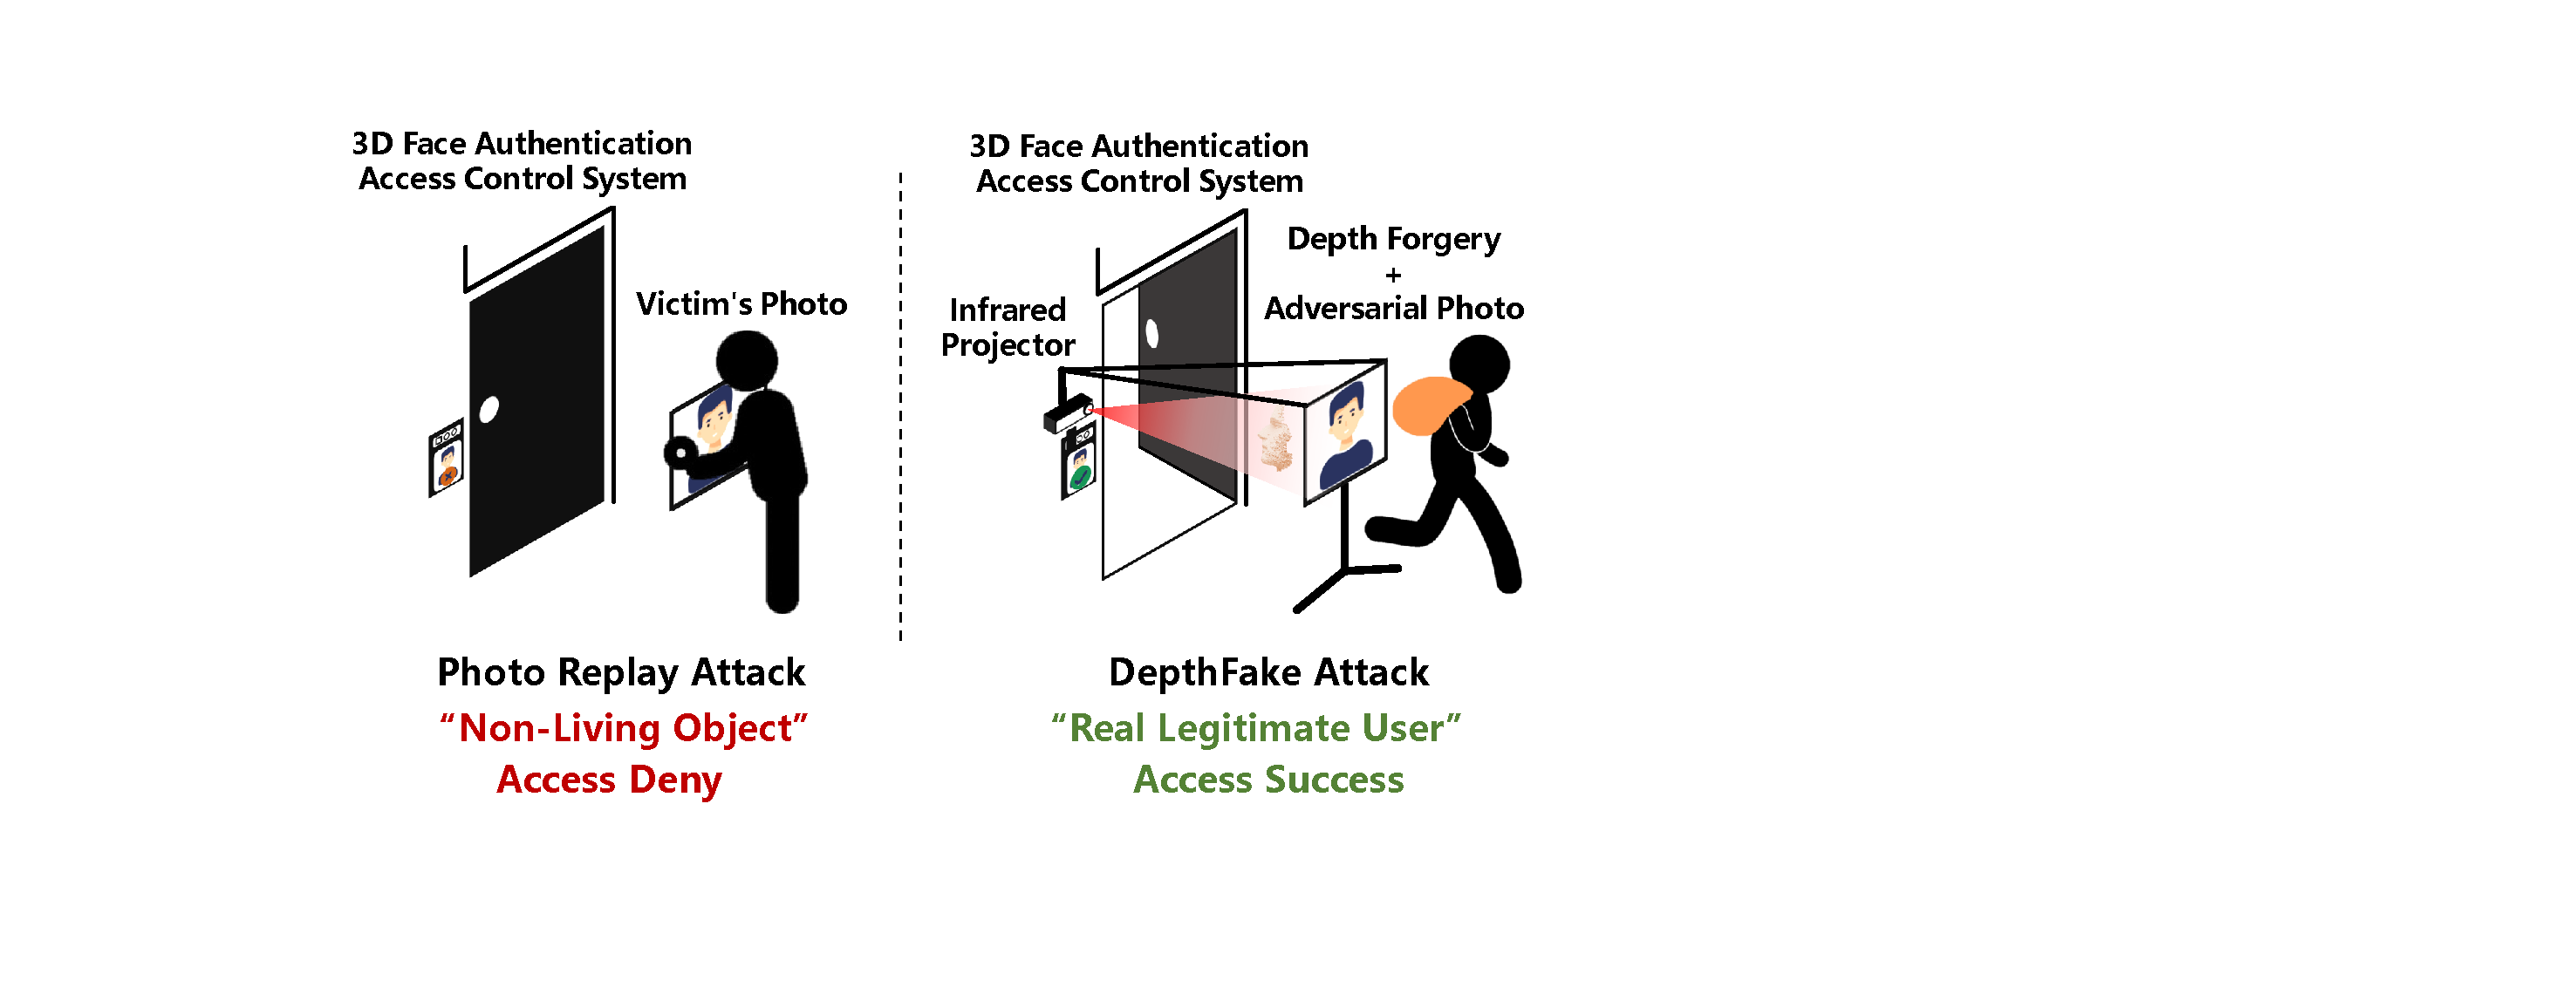
\includegraphics[width = 0.48\textwidth]{figures/intro.pdf}}
	\vspace{-0.1in}
	\caption{The \texttt{DepthFake} attack bypasses the 3D face authentication with liveness detection by projecting the structured light scatter patterns onto the 2D photo of a target victim.}
	\label{intro}
	\vspace{-0.2in}
\end{figure}

In this paper, we seek to investigate \emph{``Is it indeed impossible to spoof a 3D face authentication system using only one single 2D photo?''} Theoretically, if one can forge the depth information and replay it such that the obtained depth images and RGB images match the ones of the legitimate users, 3D face authentication can be fooled. %will obtain to empower the 2D photo with 3D properties. 
The answer is Yes. We find the key to bypassing 3D liveness detection is to forge the depth information and replay it to empower the 2D photo with 3D properties. To this end, we propose the \texttt{DepthFake} attack as shown in Fig.~\ref{intro}. The \texttt{Depthfake} attack first estimates the depth information of the victim from his public 2D photo, then spoofs the depth camera by emitting the infrared pattern which contains the depth information. At last, by aligning the 2D photo with the forgery depth, the \texttt{Depthfake} attack can successfully forge the 3D information of the victim and thus bypass the 3D liveness detection.


However, the design and implementation of \texttt{DepthFake} have several challenges in the real world  against the black-box settings on commercial face authentication systems:
(1) how to obtain the depth information from a single photo?
(2) how to convert the depth information into an infrared pattern that can spoof the structured light depth camera?
(3) how to attack under the black-box systems and physically align the depth information with a 2D photo as uniformed 3D information? 


To address the above challenges, we first propose a CNN-based deep learning model with the weighted loss function to estimate the depth of information from a single photo.
Then, we model the depth measurement process and design the mapping function that can modulate the digital depth image into the desired scatter pattern to spoof the structured light depth camera.
At last, we propose an evolutionary-based RGB adversarial attack method with color calibration, and a face region alignment scheme to form a uniformed RGB-D attack.
We validate the effectiveness of \texttt{DepthFake} attacks on three commercial face authentication systems including Tencent Cloud, Baidu Cloud, and 3DiVi, and a commercial access control device in the real world. \texttt{DepthFake} attack can achieve an overall Depth attack success rate of $78.81\%$ and RGB-D attack success rate of $58.75\%$ under various settings. In summary, our contributions include the points below:
\begin{itemize}	
	\item We identify the vulnerabilities in the 3D liveness detection module of the face authentication system, and propose to spoof a 3D  face authentication system using a single 2D photo.	
	\item We design \texttt{DepthFake},  the first attack in the real world against commercial face authentication systems by projecting the modulated structured light scatter pattern on a printed photo of a target victim.	
	\item We validate the attack effectiveness of  \texttt{DepthFake} on a commercial structured light depth camera (Astra Pro), three commercial face authentication systems (Baidu Cloud, Tencent Cloud, 3DiVi), and one commercial access control device in the real world, and achieve an overall Depth attack success rate of $78.81\%$ and RGB-D attack success rate of $58.75\%$.
\end{itemize}

The \texttt{DepthFake} attack aims to expose the potential threat in 3D face authentication systems and attempts to find a secure authentication solution. Therefore, we propose the following defense methods to prevent such threats:
(1) Randomizing scatter patterns to prevent attackers from forging depth information, which has not been implemented into current depth cameras.
(2) Improving 3D liveness detection models to detect the forgery depth information and adversarial examples.

% First, the single 2D photo captured from the victim's social media do not contain any depth information thus we need to estimate the depth image from it. Second, the estimated depth image shall be modulated into the structured light scatter pattern to spoof the depth camera for generating the forgery depth image. Third, launching attacks both in RGB and depth images to ensure the effectiveness under RGB-D liveness deteciton mode. 


%It seems impossible that a single 2D photo cannot hold the 3D features required to pass the 3D liveness detection and existing spoofing attacks~\cite{souza2018far, marcel2014handbook} indeed fall short. Essentially, we find the key to bypass the 3D liveness detection is to forge the depth information.  
%To this end, we try to use only a single 2D photo to break the 3D face authentication system, and propose the \texttt{DepthFake} attack. 
%
%The \texttt{Depthfake} attack first estimates the depth information of the victim from his public 2D photo, then forges the depth information in the real world by spoofing the structured light depth camera. In this way, a 2D photo is empowered with depth information. In addition, to enhance the attack performance against RGB-D-based liveness detection (i.e., the form of 3D livenss detection), we resort to adversarial example attacks to achieve uniformed spoofing.		


% find that a face authentication system includes a face detection phase, a liveness detection phase, and a face comparison phase, and the three phases work in serial. To bypass the 3D liveness detection, the key is to forge the depth information.

% propose the \texttt{DepthFake} attack, which uses only a single 2D photo to break the 3D face authentication system as shown in Fig.~\ref{intro}. 

%the face authentication systems usually use the RGB-D liveness detection for security purposes, the \texttt{Depthfake} attacks need to be facilitated with the capability of bypassing RGB-based liveness detection such as the edge detection or moiré-pattern check~\cite{yang2014learn, chen2020face, luo2018face}, we resort to the adversarial example attacks and add patterns such as white squares to the printed photos to achieve a flexible spoofing.	
%\texttt{DepthFake} attacks first generate the desired structured-light scatter pattern (normally IR) by measuring the displacements between the reflected and the legitimate ones. Then, the generated structured-light scatter pattern is projected onto the printed photo of the target victim to forge the depth information. 
%In this way, a 2D photo is empowered with the depth information. Our preliminary analysis in Sec.~\ref{sec:preliminary} shows that naively replaying a structured light scatter pattern can generate the depth information but has difficulty in deriving a desired one. In addition, to facilitate \texttt{DepthFake}  attacks with the capability of bypassing RGB-based liveness detection such as the edge detection or moiré-pattern check~\cite{yang2014learn, chen2020face, luo2018face}, we resort to the adversarial example attacks and add patterns such as white squares to the printed photos to achieve a flexible spoofing.	

%First, unlike traditional multi-view depth estimation methods, we obtain the depth information from a single public photo of the victim, which may introduce potential biases.
%Second, the structured light depth camera measures depth information using a specific scatter pattern, thus the depth images shall be converted to the desired scatter pattern.
%Third, the RGB adversarial examples may suffer from the colors shifted and need to align with depth images against the RGB-D liveness detection.

%To prevent 2D replay attacks, manufacturers such as Apple and Microsoft~\cite{faceid} utilize 3D liveness detection techniques to secure the authentication process, which is known as the 3D face authentication system. Specifically, it utilizes a depth camera to obtain the 3D information and identify whether the real user truly present.

% A face authentication system is a technology capable of matching a human face, usually in the form of a digital image, against a database of faces, to authenticate the legitimacy of the user. The enabled services include but are not limited to unlocking devices, securing financial payments, and physical access control to critical infrastructures. Especially, face authentication is regarded as a secure and common authentication method compared to other biometric solutions such as fingerprint authentication due to its non-contact property during the COVID-19 era.

%However, a face authentication system has been shown to be vulnerable to spoofing attacks.
%A naive but efficient idea is to use a printed photo of the legitimate user, which is also known as the 2D replay attack~\cite{chakka2011competition,anjos2011counter,raghavendra2015presentation}. To prevent such 2D replay attacks, face authentication systems nowadays are facilitated with liveness detection techniques. 
%Liveness detection requires users to participate in the authentication process, e.g., shaking their heads, or obtaining their 3D information to ensure they are truly present. In particular, due to the security and user-friendly consideration, the 3D liveness detection is being adopted by more manufacturers, such as Apple, Microsoft, etc. ~\cite{faceid}.
% !TEX root = ../main.tex
\section{Background}
\label{sec:background}
%-------------------------------------------------------------------------------
In this section, we first present the work-flow of the 3D face authentication system and then introduce the liveness detection in detail.

\subsection{3D Face Authentication}
Face authentication is a biometrical authentication scheme used to verify the identity of a user. To prevent a face authentication system from photo replay attacks, 3D face authentication is invented by adding the 3D liveness detection module. 

A standard 3D face authentication system typically employs a visible light camera and an infrared camera. When a user attempts to authenticate, RGB and depth images are captured. As shown in Fig~\ref{fas_workflow}, the 3D face authentication process has the following three steps:
%When a user attempts to access a device or system with 3D face authentication, the RGB as well as the depth images of the users are captured by the visible light camera and the infrared camera, respectively, for further authentication. A standard 3D face authentication system works in three steps as shown in Figure.~\ref{fas_workflow}.

\textbf{Step 1: Face Detection.} 
The face detection step detects and crops the face regions in the RGB and depth images. For RGB images, face detection algorithms such as multi-task convolutional neural network (MTCNN) \cite{zhang2016joint} are used to locate the face area in the RGB images and output the bounding-box coordinates. Based on the face area in an RGB image, the face area in a depth image is extracted by mapping the face bounding-box coordinates of a RGB image to that of the depth image.

\textbf{Step 2: Liveness Detection.} The liveness detection step analyzes the liveness properties, such as the edges, textures, Moiré patterns
 from an RGB image and the 3D depth information from a depth image. 
This step aims to defend against spoofing attacks such as photo replay attacks, video replays attack, and mask-wearing attacks~\cite{chakka2011competition,anjos2011counter,raghavendra2015presentation, bhattacharjee2018spoofing, nesli2013spoofing}.

\textbf{Step 3: Face Comparison.} After the liveness detection step, the face comparison step employs comparison algorithms such as FaceNet~\cite{schroff2015facenet} to verify if the user is the legitimate one. The comparison algorithms often extract a feature vector from the newly captured face images and calculate the similarity distance between it and the enrolled feature vector stored in the database. Note that face comparison only relies on the RGB images because of their high resolution.

\textcolor{red}{From the workflow of the face authentication system, we find the key to fooling it with a 2D photo is to bypass the liveness detection since a photo from the legitimate user can naturally bypass the other two steps.}
%From the work-flow of the face authentication system, we find that the key to fool a 3D face authentication system is to bypass its liveness detection module. 
In the following, we introduce the liveness detection in detail.

\begin{figure}[pt]
	\centerline{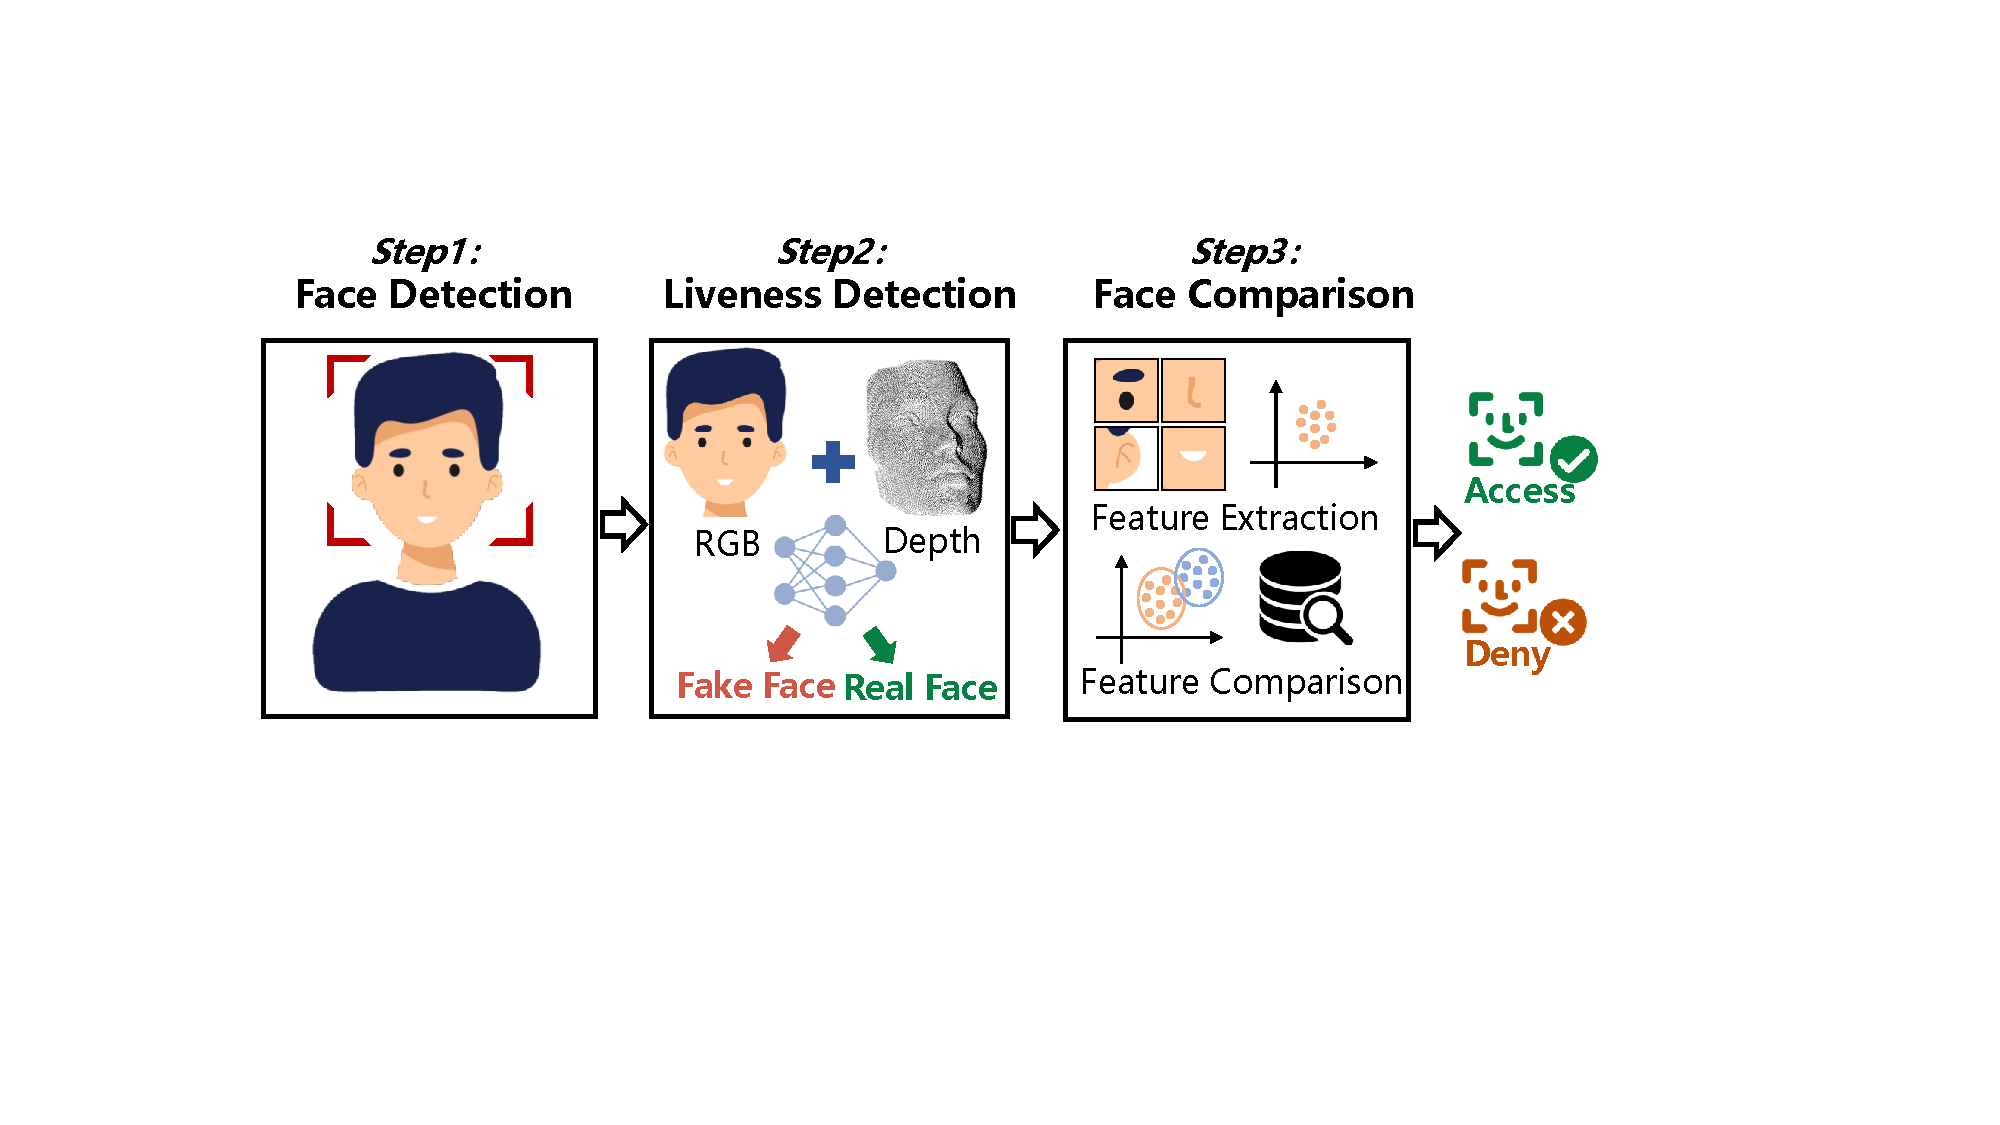
\includegraphics[width = 0.5\textwidth]{figures/face_auth_workflow.pdf}}
	\vspace{-0.15in}
	\caption{The 3D face authentication system first detects faces in the captured RGB and depth images, then determines whether those faces are from real people, and finally verifies whether they are from legitimate users.}
	\label{fas_workflow}
	\vspace{-0.15in}
\end{figure}

\subsection{Liveness Detection}
Liveness detection determines whether the person to be authenticated is a live person or not. 
It aims to reject non-living objects that try to obfuscate the face authentication system, e.g., a printed photo.
Existing liveness detection methods include two categories: 
(1) Active liveness detection requires the user to perform a predefined action, e.g., blink or nod. This method needs multiple captured images to recognize a pre-defied action and therefore is commonly used in cloud-service-based face authentication due to its extra requirements on computing resources. 
(2) Passive liveness detection, on the contrary, only uses one-shot images to determine whether the user is alive. 
Since passive liveness detection is lightweight and requires little user interaction, it is a popular method used nowadays in smartphones, smart locks, access control devices, etc~\cite{chakraborty2014overview}. Thus, in this paper, we target the 3D liveness detection in a passive manner. 

\subsection{3D Passive Liveness Detection}

3D passive liveness detection utilizes both RGB and depth images, and it may use one of the following types of depth cameras: (1) structured light camera which uses the infrared scatter pattern to encode depth information, (2) time-of-flight (ToF) camera which calculates the depth by recording the infrared light echo time, and (3) binocular stereo camera, which obtains depth information by matching different perspectives photos taken by two cameras.
Among them, the structured-light-based depth camera is the most widely used one for face authentication systems, because of its high resolution, insensitivity to visible light, and low cost. For instance, it is used by FaceID~\cite{han2007face,bud2018facing}, and Smartlock\cite{waseem2020face}. Since the structured-light-based depth cameras are reported to occupy  almost 25\% among all the depth camera market~\cite{3dcameramarket},
in this paper, we focus on the passive liveness detection systems using structured-light-based depth cameras. 
%Nevertheless, the methodology of \texttt{DepthFake} can be applied to other liveness detection methods.

\begin{figure}[pt] 
	\centerline{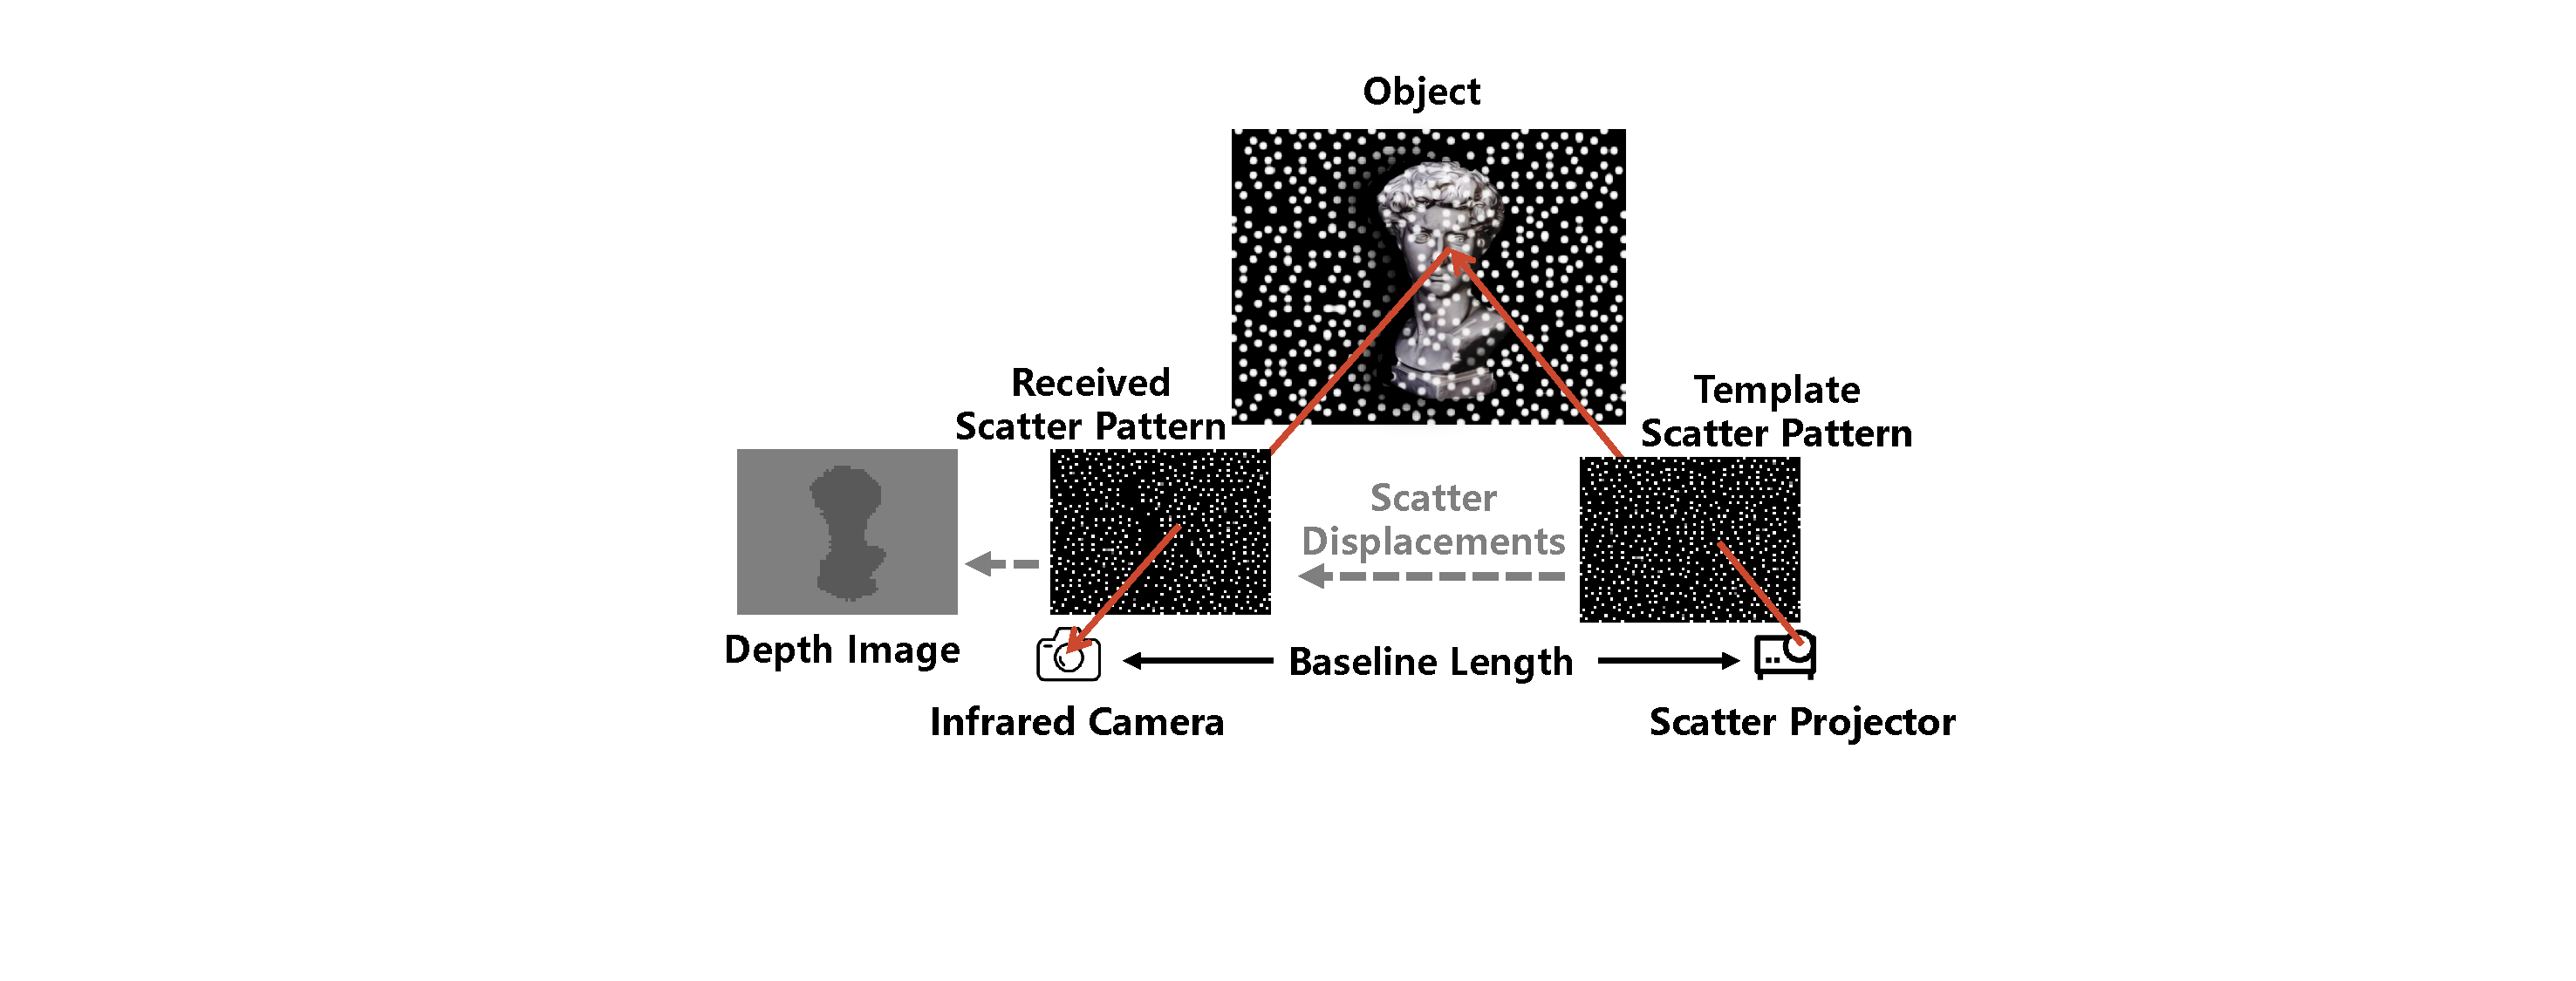
\includegraphics[width = 0.48\textwidth]{figures/structured_light_camera.pdf}}
	\vspace{-0.1in}
	\caption{The structured light depth camera actively projects a constant scatter pattern to the object, e.g., a face, then captures the reflected scatter pattern and calculates the depth of the target by measuring its displacement from the template scatter pattern for each scatter point. }
	\label{depth_camera}
	\vspace{-0.15in}
\end{figure}


%A structured-light-based 3D passive liveness detection module (3D liveness detection module in short) consists of both hardware and software components.
%, where the former captures the face information of the user pending authentication while the latter processes the information and makes decisions.
%\textbf{Hardware.}
%The hardware component  of a 3D liveness detection module include a visible camera and a structured light depth camera, which capture the RGB and depth images of a legitimate user  simultaneously~\cite{zanuttigh2016time, daneshmand20183d}. 
\textbf{Structured-light-based 3D Liveness Detection.} A standard structured light depth camera contains a scatter projector and an infrared camera, as shown in Fig.~\ref{depth_camera}. Most scatter projector projects a constant infrared pattern containing tens of thousands of scatter points. During calibration in the factory, the infrared camera captures the scatter patten at the reference depth plane and stores it as a template scatter pattern. To obtain a depth image of a user,  the infrared camera captures the reflected scatter pattern, which is distorted due to the different depths of the face, and it calculates the depth information by measuring the displacements between each scatter point with the one stored in the template scatter pattern.


%
%When capturing a depth image of a target user, the reflected scatter pattern will be distorted due to the different depths of the face. Then, the infrared camera will capture the distorted scatter pattern and calculate the depth information by measuring the displacements between each scatter point with the one stored in the template scatter pattern.

To illustrate how the structured light depth camera calculates the depth information from scatter point displacements, we consider a single scatter point.
% For simplicity, we take the depth calculation for a single scatter point as an example to illustrate how the structured light camera measures the depth from scatter displacements. 
As shown in Fig.~\ref{imaging_mechanism}, as an infrared beam of $x_p$ is reflected at the plane of reference depth $d_{ref}$ and tatget depth $d_t$, the scatter points on the image sensor of infrared camera can be denoted as $x_{ref}$ and $x_{t}$, respectively. 
%a scatter point $x_p$ reflected by the planes of  reference depth $d_{ref}$ and tatget depth $d_t$ are denoted as $x_{ref}$ and $x_{t}$ on the imaging plane of the infrared camera.
Based on the rule of the similar triangle, we can calculate $d_t$ as follows:
\begin{equation}
	d_t= \frac{d_{ref}Lf_c}{Lf_c - d_{ref}\Delta x_c}
	\label{d_cal}
\end{equation}
where $\Delta x_c=x_{ref}-x_{t}$ is the displacement between $x_{ref}$ and $x_{t}$. The baseline length $L$, the focal length $f_c$, and reference depth $d_{ref}$ are constant and known to the depth camera. Thus,  the camera can obtain the depth of a single point and multiple points across the entire face.

%Based on the similar triangles rule, we can calculate $x_{ref}$ and $x_{t}$ as follows:
%
%\begin{equation}
%	x_{ref}=\frac{f_c}{d_ref}(L-\frac{x_pd_ref}{f_p}) 
%	\label{xc1_cal}
%\end{equation}
%\begin{equation}
%	x_{t}=\frac{f_c}{d_t}(L-\frac{x_pd_t}{f_p}) 
%	\label{xc2_cal}
%\end{equation}
%where $f_c$ and $f_p$ are the focal length of the infrared camera and projector, and  $L$  is the baseline length (distance) between infrared camera and projector. 
%Based on them, we can calculate ${d_t}$ as follows:
%\begin{equation}
%	%\frac{1}{d_1} - \frac{1}{d_2} = \frac{\Delta x}{Lf_c} 
%	d_t= \frac{d_refLf_c}{Lf_c - d_ref\Delta x_c}
%	\label{d_cal}
%\end{equation}
%where $\Delta x_c=x_{ref}-x_{t}$ is the displacement between $x_{ref}$ and $x_{t}$. The baseline length $L$, the focal length $f_c$, and reference depth $d_ref$ are constant and known to the depth camera. In such way, the camera can obtain the depth of a single point and even a complete face.


\begin{figure}[!t]
	\centering
	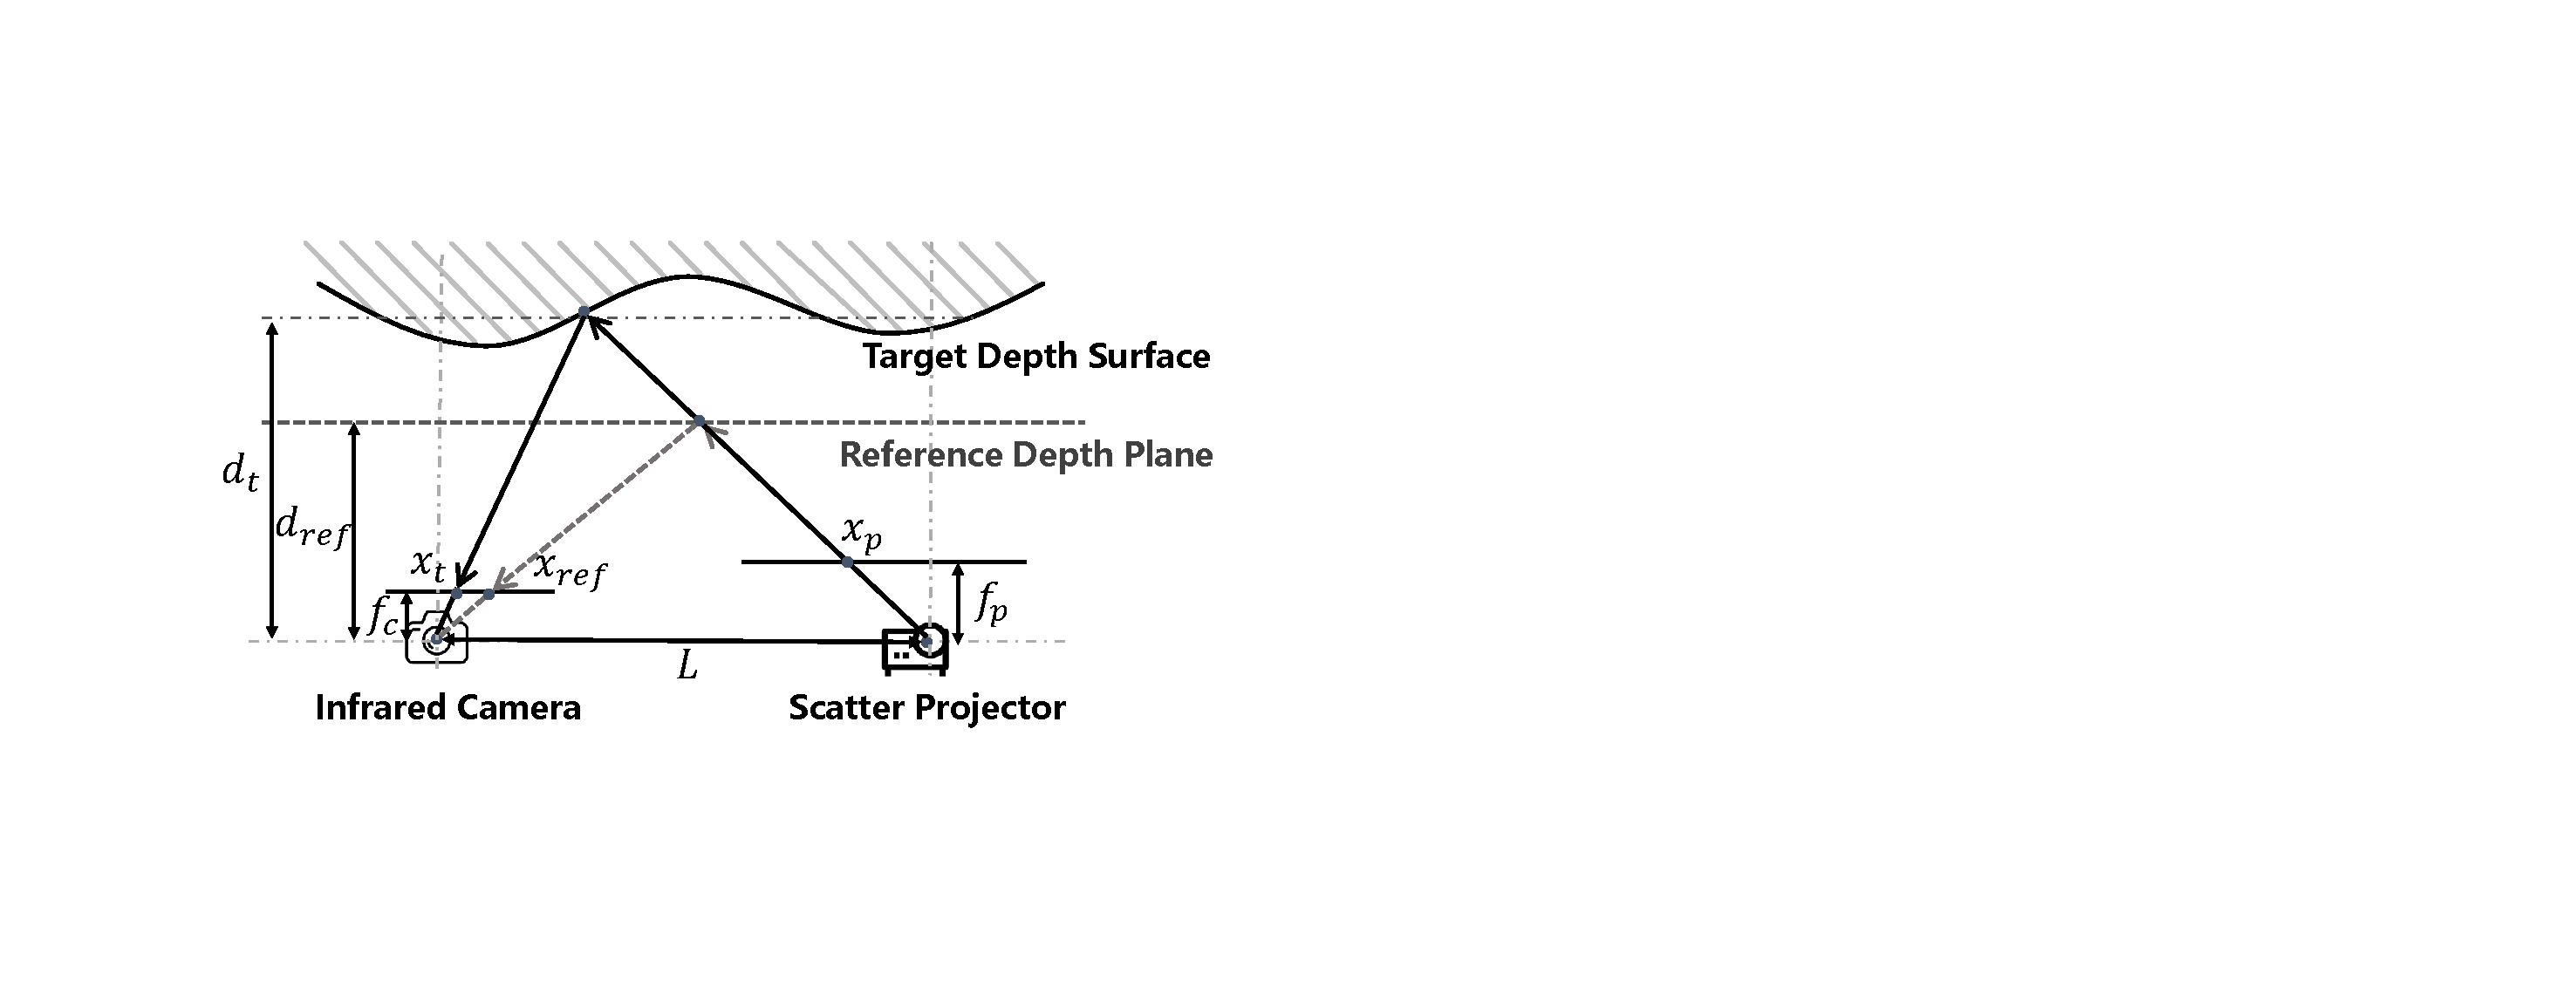
\includegraphics[width=0.48\textwidth]{figures/imaging_mechanism.pdf} 
	\vspace{-0.1in}
	\caption{Imaging mechanism of the structured light depth camera. The scatter projector projects the scatter point to the target depth plane, then the infrared camera captures the reflected scatter point and calculates the target depth by measuring its displacement to the template scatter point. }
	\label{imaging_mechanism}
	\vspace{-0.15in}
\end{figure}

After obtaining RGB and depth images, the 3D liveness detection module utilizes both of them to determine the liveness.
For an RGB image, deep learning algorithms such as Convolution Neural Networks (CNNs)~\cite{yang2014learn, chen2020face, luo2018face} or Vision Transformer (Vit)~\cite{george2020effectiveness}, are used to extract features, e.g., edges, textures, Moiré patterns or features in the frequency domain in the RGB image, to determine whether the RGB stands for a real person.
For a depth image, the region with the face is extracted by mapping to the RGB image, and then feature point matching algorithms~\cite{goswami2014rgb} or CNNs~\cite{george2021cross, te2020exploring} are used to determine whether the face belongs to a real person by detecting the special geometric structure of the face. 

%\textbf{Hardware.} The
%3D liveness detection module uses a visible camera to capture the RGB image of a legitimate user and a structured-light depth camera~\cite{zanuttigh2016time, daneshmand20183d} to capture the depth image at the same time. 
%A standard structured-light depth camera contains a scatter projector and an infrared camera, as shown in Fig.~\ref{depth_camera}.
%During capturing depth images,  the projector first projects a fixed infrared scatter pattern to the target, which will suffer from different deformations due to the different depths of the target. Then, the infrared camera will capture the reflected scatter pattern from the object and compare it with the projected scatter pattern.  By measuring the displacement of each scatter with the disparity estimation algorithm~\cite{fanello2016hyperdepth}, it calculates the depth of the target.

%\textbf{Software.} After obtaining RGB and depth images at the same time, 3D liveness detection module utilizes both of them for decisions.
%For RGB images, it uses deep learning algorithms, e.g., Convolution Neural Networks (CNNs)~\cite{yang2014learn, chen2020face, luo2018face} or Vision Transformer (ViT)~\cite{george2020effectiveness}, to extract features such as edges, textures, moiré patterns or features in the frequency domain,  and then utilizes a binary classifier to determine them as true or fake faces with confidence scores.
%For depth images, it first maps it with the RGB image and locates the region of the face. Then, it uses feature point matching~\cite{goswami2014rgb} or CNNs~\cite{george2021cross, te2020exploring} to determine whether the face belongs to a real person by detecting the special geometric structure of the human face. 




%\textbf{Hardware. }
%3D passive liveness detection uses a visible camera to capture the RGB image of a legitimate user and a structured-light depth camera~\cite{zanuttigh2016time, daneshmand20183d} to capture the depth image at the same time. 
%A standard structured-light depth camera contains a scatter projector and an infrared camera, as shown in Fig.~\ref{depth_camera}.
%During capturing depth images,  the projector first projects a fixed infrared scatter pattern to the target, which will suffer from different deformations due to the different depths of the target. Then, the infrared camera will capture the reflected scatter pattern from the object and compare it with the projected scatter pattern.  By measuring the displacement of each scatter with the disparity estimation algorithm~\cite{fanello2016hyperdepth}, it calculates the depth of the target.
%
%\textbf{Software. } After obtaining RGB and depth images at the same time, 3D liveness detection utilizes both of them for decisions.
%For RGB images, it uses deep learning algorithms, e.g., Convolution Neural Networks (CNNs)~\cite{yang2014learn, chen2020face, luo2018face} or Vision Transformer (ViT)~\cite{george2020effectiveness}, to extract features such as edges, textures, moiré patterns or features in the frequency domain,  and then utilizes a binary classifier to determine them as true or fake faces with confidence scores.
%For depth images, it first maps it with the RGB image and locates the region of the face. Then, it uses feature point matching~\cite{goswami2014rgb} or CNNs~\cite{george2021cross, te2020exploring} to determine whether the face belongs to a real person by detecting the special geometric structure of the human face. 

%(2) IR-based liveness detection, which actively projects infrared light to target object and identifies the real face through comparing the difference of reflection features between the real human face and other spoofing materials. 
%(3) RGB+IR liveness detection, which combines the advantages of RGB-based and IR-based liveness detection and can work in different lighting conditions. 
%3D passive liveness detection is RGB-Depth-based (RGBD-based in short), which uses the depth information as an auxiliary feature in anti-spoofing. The algorithm reconstructs a 3D structure from depth image and uses it to determine whether the target is a real person or not.

%\subsection{Spoofing Attacks against Face Authentication}
%
%Existing spoofing attacks against face authentication mainly focus on the face comparison step, i.e., approximating the feature vector of a legitimate user in the face feature representation space. In this area, much work~\cite{sharif2016accessorize, singh2022powerful, nguyen2020adversarial, guo2021meaningful, komkov2021advhat, zolfi2021adversarial} has demonstrated the feasibility of fooling deep-learning-based face comparison algorithms with adversarial examples, which can render the algorithms identify an adversary as a legitimate user.However, those attacks mainly work for RGB images and may lose their attack capabilities when depth features are used \cite{belli2022personalized}.
%Another aspect of spoofing face authentication is to deceive its 3D liveness detection. Existing work to achieve it is using an ultra-realistic 3D face mask~\cite{bhattacharjee2018spoofing}, but it requires a detailed 3D modeling of the victim and a high cost (over $\$4,000$).In this paper, we investigate the possibility of fooling face authentication with a low-cost printed photo.





%Face spoofing attacks use artifacts to spoof liveness detection systems. The most common way is the replay attack. The current replay attacks usually use high-precision printer to print the photo or high-resolution monitor to replay the video of the victim. Additionally, there are attackers who design ultra-realistic face mask to spoof liveness detection. However, the multi-modal liveness detection can prevent these attacks by identifying the specific texture or optical features.  
%
%There are other face spoofing attacks are emerging nowadays which taking over the camera feed and injecting the pre-designed image or video. Deepfake attack is one of the injecting attack, which uses synthetic face data and injects it into the camera. However, injecting attacks are all need intrusion into the hardware or software of liveness detection systems and are difficult to deploy in the real world.
%
%Therefore, in this paper, we conduct replay attacks which are more easier to deploy in the real world and propose different replay attacks for different modalities to against multi-modal liveness detection systems.
% !TEX root = ../main.tex
\section{Threat Model}


\begin{figure*}[pt]
	\centerline{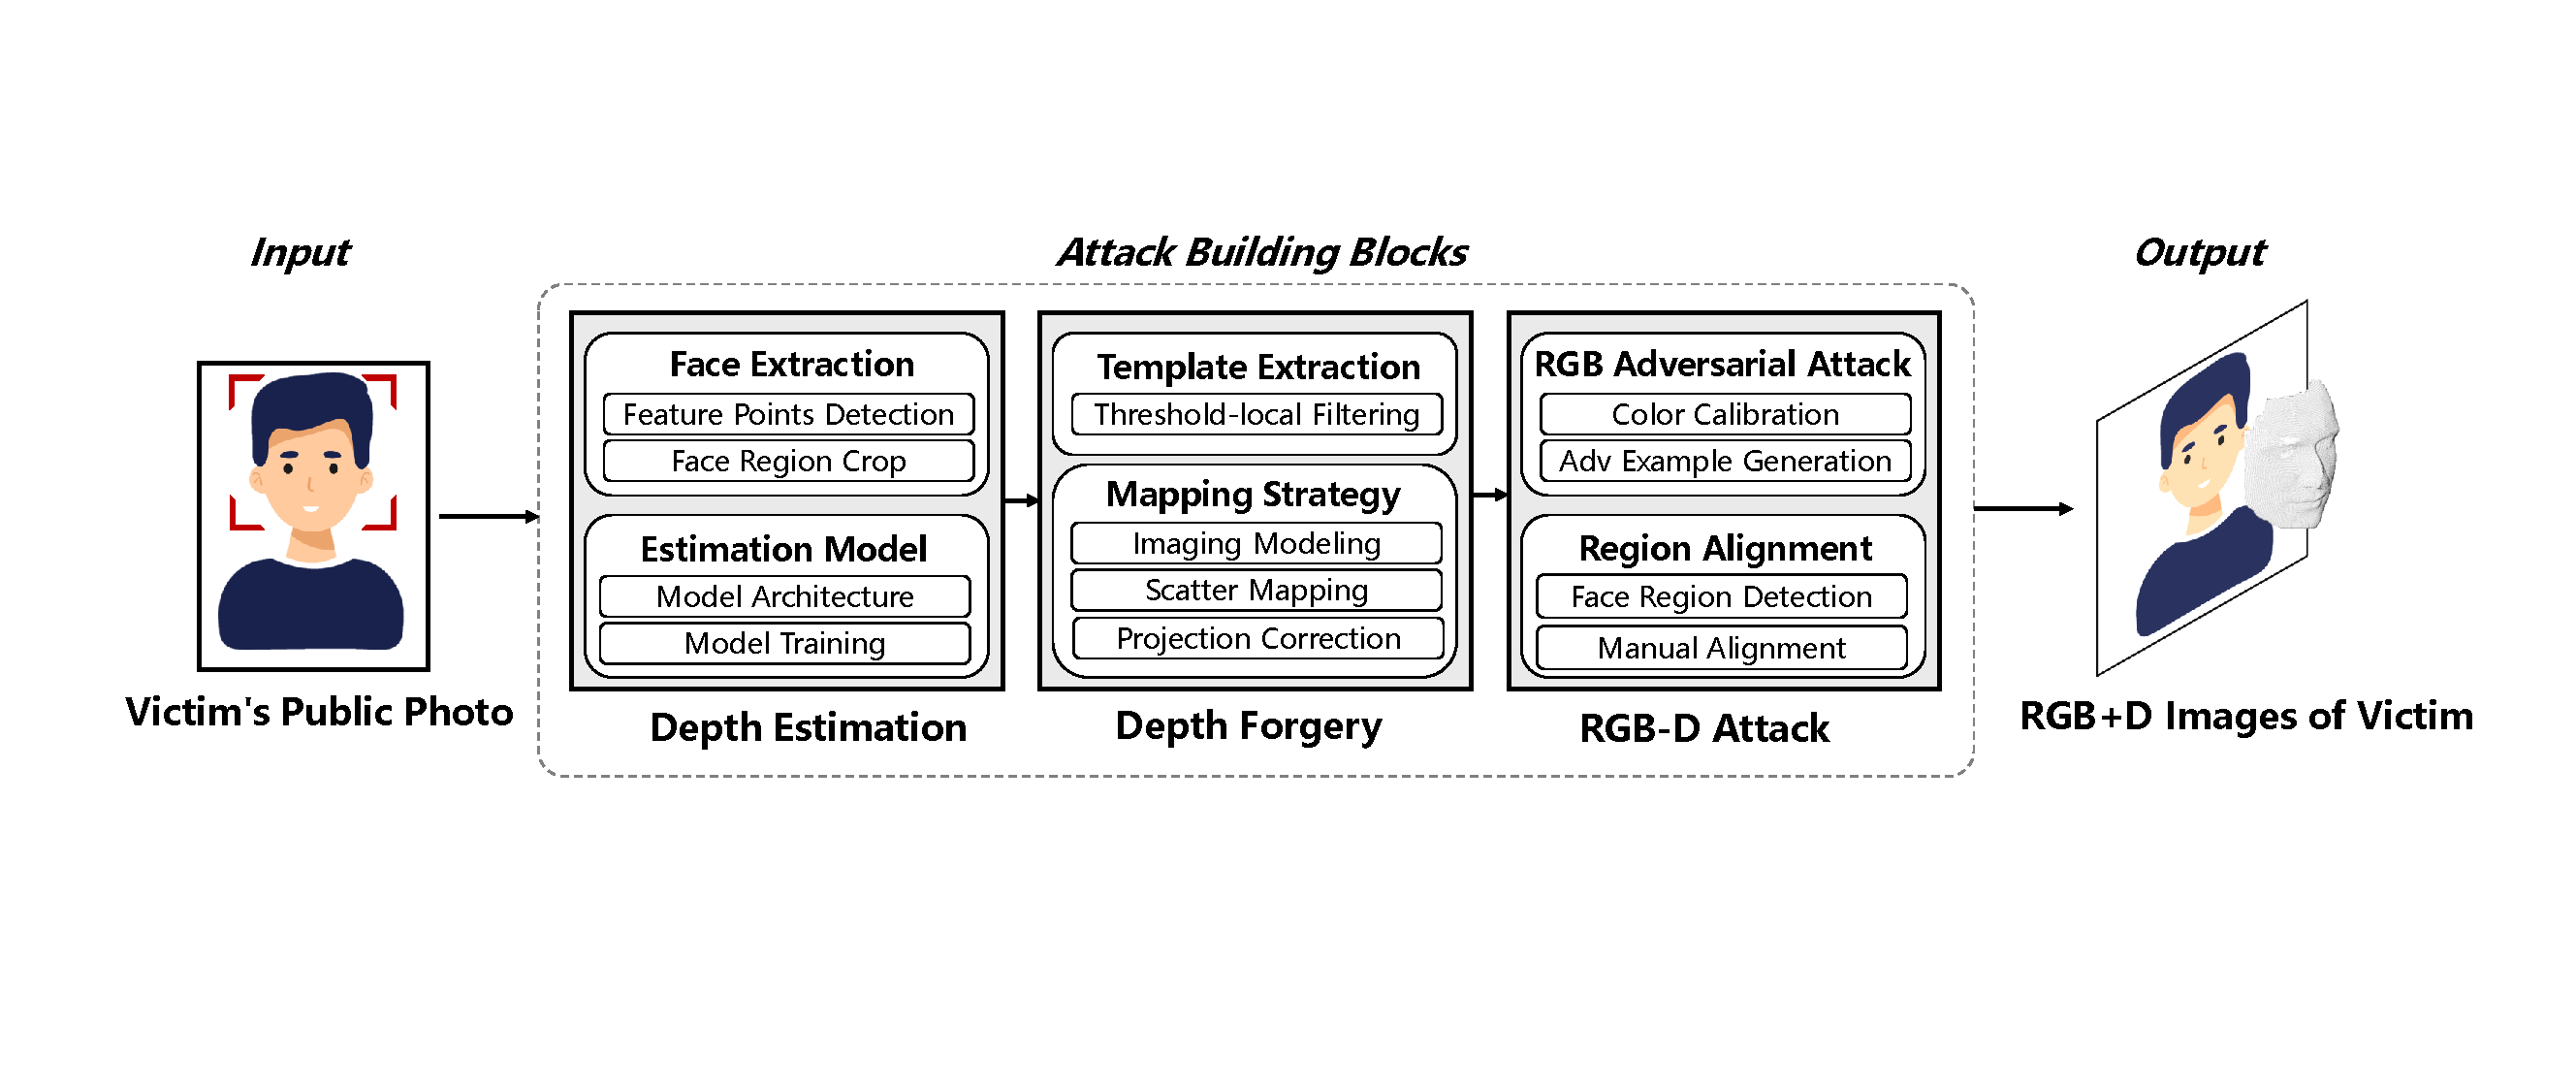
\includegraphics[width = \textwidth]{figures/overview.pdf}}
	\vspace{-0.1in}
	\caption{Overview of \texttt{DepthFake} attack: The adversary first estimates the depth image from the victim's 2D photo. Then, she extracts the template scatter pattern and modulates the depth information to the desired scatter pattern for depth forgery. To finally bypass the 3D face authentication, the adversary also uses the RGB adversarial attack and aligns it with the forgery depth image to launch a uniformed RGB-D attack.}
	\label{overview}
	\vspace{-0.15in}
\end{figure*}

The goal of the \texttt{DepthFake} attack is to spoof a 3D face authentication system using a 2D photo by bypassing its 3D liveness detection module. We consider the following attack scenario: An adversary wants to get inside a confidential place where the access control device is equipped with  a 3D face authentication system. To achieve it, she launches a \texttt{DepthFake} attack by placing the target victim's printed photo in front of the camera of the authentication system, as shown in Fig.~\ref{intro} and projecting the carefully-crafted scatter pattern onto the printed photo to spoof the 3D face authentication system.
%In this paper, we conduct two type of attacks as following: 
%
%\textbf{Depth Attack.} 
%
%\textbf{RGB-D Attack.} 

% The goal of \texttt{DepthFake} attack is to spoof the 3D face authentication system using a printed  photo by bypassing its 3D liveness detection module. Imaging a scenario where an adversary wants to get inside a confidential location where the 3D face authentication is deployed, or a scenario where the adversary wants to unlock a victim's smartphone which uses 3D face authentication. In either scenario, the adversary launches the \texttt{DepthFake} attack by projecting the deliberately crafted structured-light scatter pattern on an the photo of the victim user.

The victim authentication system is supposed to employ both RGB and depth liveness detection techniques. To achieve the aforementioned attack, the adversary has the following capabilities:

\textbf{Depth Camera Awareness.}
The adversary can acquire a depth camera of the same model as the one used in the victim system. The attacker can obtain the template scatter pattern of the victim system from the substitute camera by capturing an infrared image.


\textbf{Public Photo Access.}
The adversary can obtain a  2D photo of the victim from  public platforms such as his social medias like Facebook, Twitter, WeChat, etc.
%\textbf{Camera and User Information Awareness.} 
%The adversary can acquire a depth camera of the same model as the one used in the victim system. Then, the adversary can utilize the camera to capture the template scatter pattern. Besides, the adversary can obtain the victim's 2D photo from the public platforms such as his social media or public databases.
%The adversary can acquire a camera of the same model as the one used in the victim system. Then, the adversary can utilize the camera to capture an RGB image and a depth image of the legitimate user.

\textbf{Physical Access to the Victim Device.} The adversary can physically get close to the victim system and set up the attack device, i.e., the printed photo displayed on a board and the infrared projector.


\textbf{Black-box Setting.} 
We assume the target liveness detection systems is a black-box. For depth forgery attacks, the adversary does not require any feedback from the victim systems, and for RGB liveness detection attacks, we assume she can obtain the confidence score from the victim system, which is a common assumption in most prior work~\cite{guo2019simple}.

% When deploying \texttt{DepthFake}, we only need to obtain the authentication results from the authentication system during the estimation and projection of the depth image. However, when the authentication system is extended to RGB-D mode, the adversary should also obtain the corresponding confidence scores of liveness detection. And there is no need to acquire prior knowledge of the authentication system, i.e., network architecture, parameters, etc. This is reasonable, as various commercial face authentication SDKs or APIs such as Tencent Cloud and Baidu Cloud only provide detection results or confidence scores, without exposing the model.



% % !TEX root = ../main.tex
\section{Preliminary Analysis}
\label{sec:preliminary}
In this section, we present the basic ideas and the preliminary results of our attacks.


\begin{figure*}[htbp]
	\centering
%	\subfigure[Original RGB image]{
%		\includegraphics[width=0.23\textwidth]{figures/preanalysis_rgb_1.png} 
%	}
	\subfigure[Printed RGB photo]{
		\includegraphics[width=0.28\textwidth]{figures/preanalysis_rgb_2.png} 
	}
	\subfigure[Digital adversarial example]{
		\includegraphics[width=0.28\textwidth]{figures/preanalysis_rgb_3.png} 
	}
	\subfigure[Printed adversarial photo]{
		\includegraphics[width=0.28\textwidth]{figures/preanalysis_rgb_4.png} 
	}
\vspace{-0.15in}
	\caption{Spoofing RGB-based liveness detection with adversarial photos. (a) Printed photo of a legitimate user with a RGB confidence score: 0.06, (b) Digital adversarial example with a RGB confidence score: 0.96, and (c) Printed adversarial photo with a RGB confidence score: 0.34. }
	\label{preanalysis_rgb}
	\vspace{-0.15in}
\end{figure*}

\begin{figure*}[pt]
	\centering
			\subfigure[Original RGB image]{
			\includegraphics[width=0.28\textwidth]{figures/color1115200905_1.png} 
		}
		\subfigure[Original depth image]{
			\includegraphics[width=0.28\textwidth]{figures/preanalysis_depth_1.png} 
		}
		\subfigure[Replayed depth image]{
			\includegraphics[width=0.28\textwidth]{./figures/preanalysis_depth_2.png} 
		}
%	\subfigure[Replayed depth image with noise reduction]{
%		\includegraphics[width=0.23\textwidth]{./figures/preanalysis_depth_3.png} 
%		}
	\vspace{-0.15in}
		\caption{Spoofing depth-based liveness detection by replaying structured-light patterns. (a)  Original RGB and (b) depth images with a RGB-D confidence score: 0.99, and (c) Replayed depth image with a RGB-D confidence score: 0.02. }
			\vspace{-0.15in}
		\label{preanalysis_depth}
%	\begin{minipage}[t]{0.5\textwidth}
%		\subfigure[Original infrared image]{
%			\includegraphics[width=0.46\textwidth]{figures/preanalysis_ir_1.png} 
%		}
%		\subfigure[Replayed infrared image]{
%			\includegraphics[width=0.46\textwidth]{figures/preanalysis_ir_2.png} 
%		}
%		\caption{The infrared image replay for IR modality. (a) the original infrared image of legitimate user with liveness confidence score : 0.99; (b) the infrared image replayed through infrared projector with livness confidence score : 0.99.}
%		\label{preanalysis_ir}
%	\end{minipage}
\end{figure*}

\subsection{Basic Idea}
In this paper, we investigate the feasibility of spoofing face authentication with a printed photo by bypassing its 3D liveness detection.
Since 3D liveness detection utilizes both the RGB and depth information for detection, we shall bypass its RGB and depth detection models simultaneously.  

For the RGB-based liveness detection model, it can detect photos by analyzing their edges, textures, and moire patterns in normal circumstances. However, since those models are usually based on deep learning algorithms, they have the possibility of being vulnerable to adversarial attacks. Thus, a naive trial is to utilize printed adversarial photos to bypass it. 


For the depth-based liveness detection model, it calculates the depth information by measuring the displacement of the reflected scatter pattern and the original scatter pattern, and uses the special geometric structure of the human face to determine whether the face image is from a real human face.
However, the infrared camera only captures infrared images and does not identify the source of the scatter patterns. As a result,  we may create forged depth information by projecting artificial scatter patterns. 



In the following, we present the preliminary results of the aforementioned ideas.
\subsection{Preliminary Results }

\textbf{Spoofing RGB-based Liveness Detection.} \texttt{DepthFake} utilizes adversarial noises on photos to spoof against the RGB-based liveness detection.
To investigate, we conducted a feasibility test by generating adversarial examples against the RGB module of a commercial liveness detection SDK, i.e., the Baidu Cloud SDK. Specifically, we first captured an RGB image of a legitimate user and  printed it out as a spoofed photo, then we used a black-box adversarial attack method called SimBA \cite{guo2019simple} to generate an adversarial example in the digital world, and finally printed it out as the adversarial photo to investigate whether it can bypass the liveness detection in the real world. 

From the results in Fig.~\ref{preanalysis_rgb}, we find that the RGB-based liveness detection model of the Baidu Cloud SDK does suffer from adversarial attacks. An adversarial example in the digital world can bypass the RGB-based liveness detection with a score of 0.96. Although its attack effectiveness decreases after being printed, it can still get a score of 0.34, higher than that of a printed photo without adversarial perturbations (0.06). 

By comparing the adversarial example in the digital world (Fig.~\ref{preanalysis_rgb} b) and the printed adversarial photo in the real world (Fig.~\ref{preanalysis_rgb} c), we find that the color distortion caused by the printing-capturing process impairs the attack effectiveness. As a result, to guarantee an effective photo attack in the real world, simply generating an adversarial example is not enough. More work shall be done on improving its robustness in the real world by reducing the impacts from color distortions caused by printing and capturing.


\begin{figure*}[pt]
	\centerline{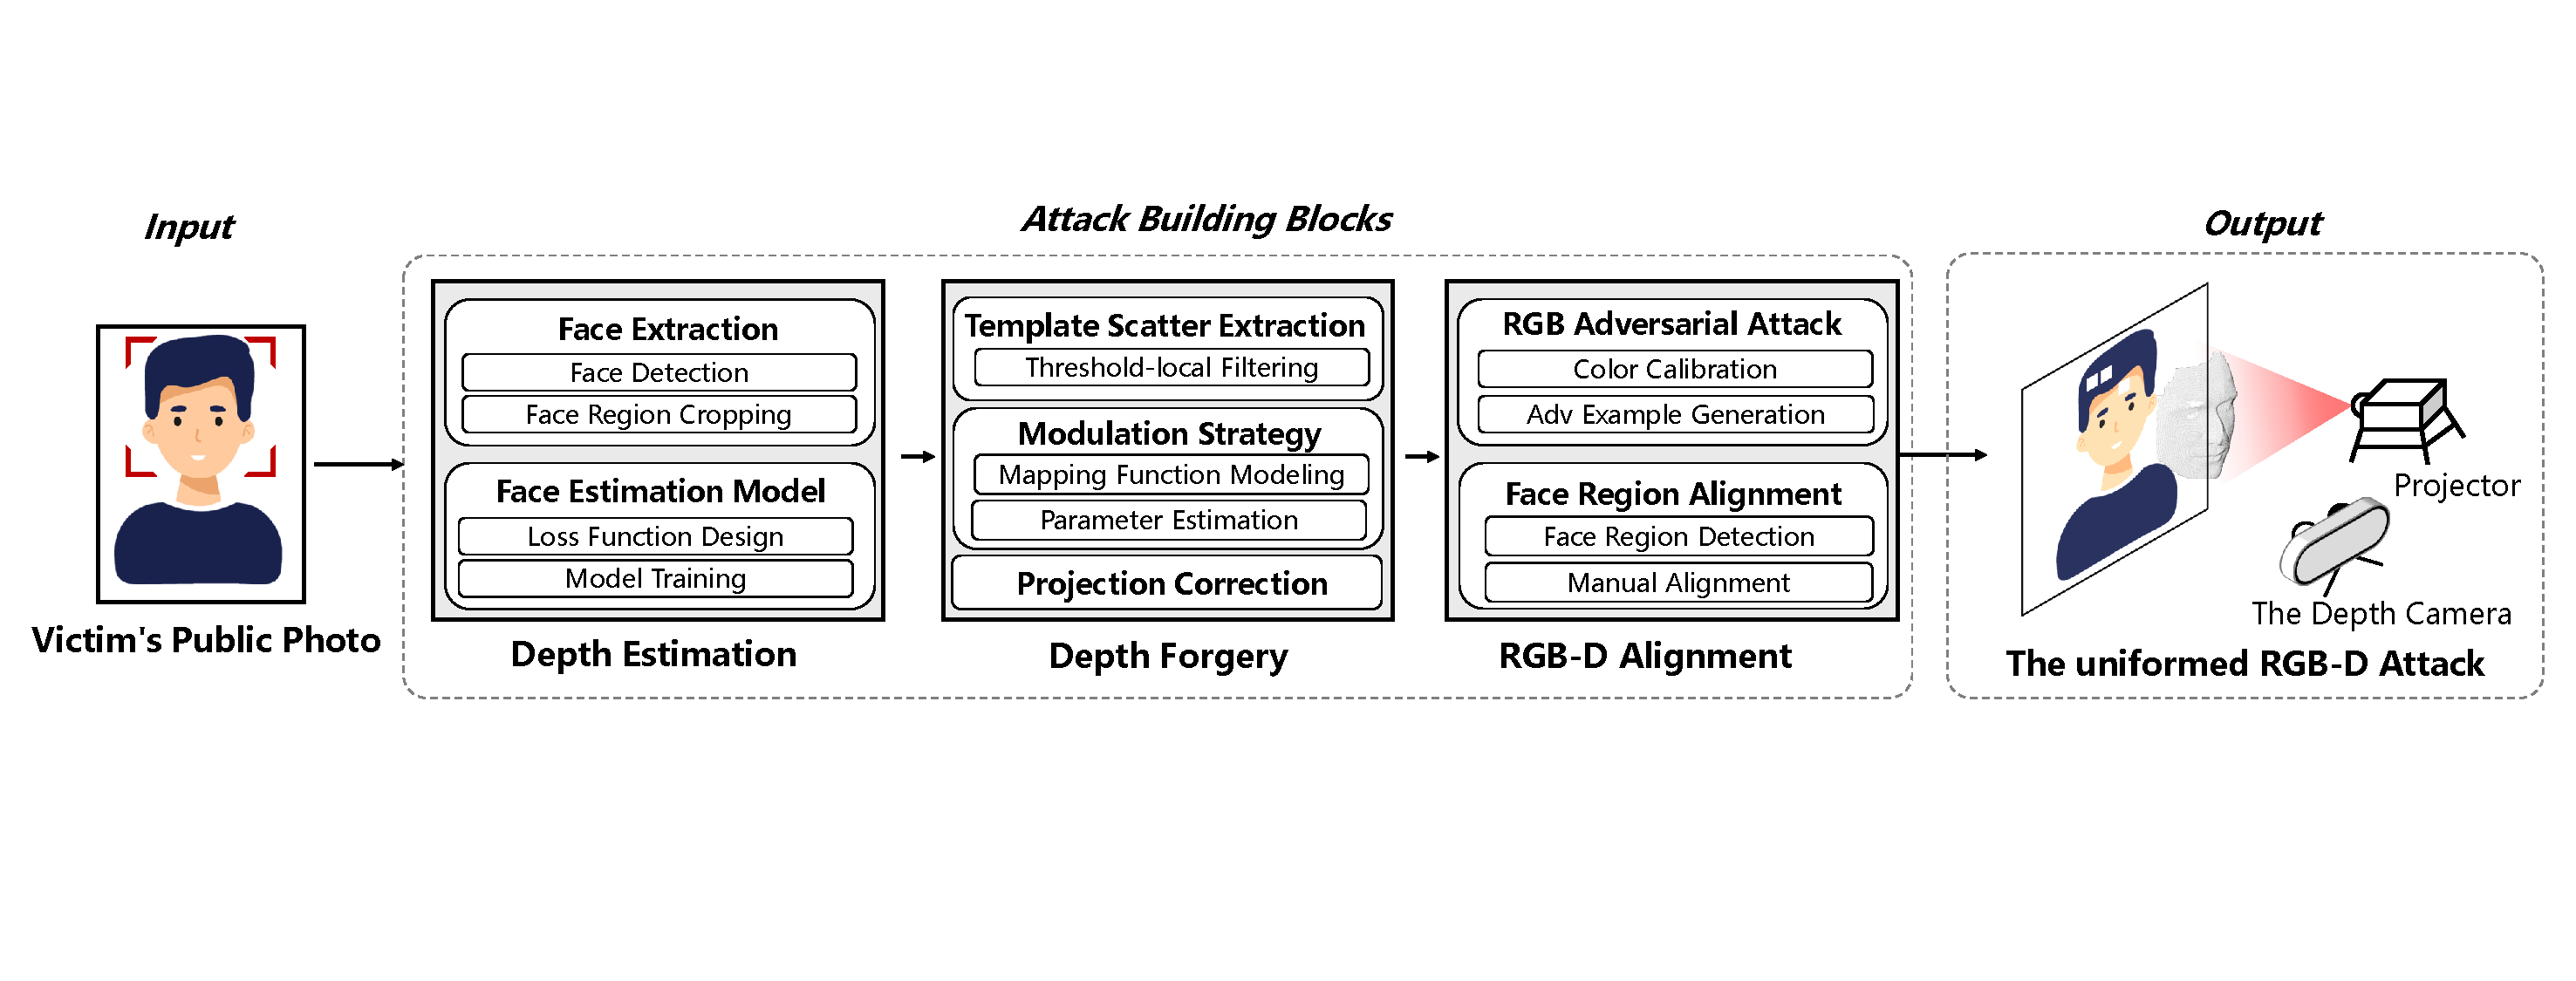
\includegraphics[width = \textwidth]{figures/overview_1.png}}
	\vspace{-0.15in}
	\caption{Overview of \texttt{DepthFake} attack: The adversary first captures a legitimate user's face information with a 3D camera. Then, she uses the face information to generate an adversarial photo and a structured-light scatter pattern projected through an infrared projector to spoof the 3D liveness detection and thus the face authentication system. }
	\label{overview}
		\vspace{-0.15in}
\end{figure*}

\textbf{Spoofing Depth-based Liveness Detection.} \texttt{DepthFake} replays the structured-light patterns to spoof against depth-based liveness detection.
To investigate this idea, we used a structured-light 3D camera Orbbec Astra Pro~\cite{da2020comparison} to capture the infrared scatter pattern reflected by a legitimate user. 
Then, we covered the scatter projector of the structured-light depth camera and used an external infrared projector DLP4500SL02 Evaluation Module~\cite{chong2017intraoperative} to replay the captured scatter pattern to forge the depth information.
The results shown in Fig.~\ref{preanalysis_depth} demonstrate that with the replayed depth image, the confidence score of 3D liveness detection (RGB-D) drops from 0.99 to 0.02.  The reason is that the replayed scatter pattern cannot form the depth of a human face directly since it suffers from noises from background objects during recording. 
%To address it, we perform Histogram Equalization~\cite{abdullah2007dynamic} to reduce the noises in the recorded scatter pattern, which can increase the confidence score from 0.02 to 0.25.

Therefore, simply replaying a structured-light scatter pattern recorded from a  legitimate user can generate the depth information but is not sufficient to forge a human face. More work shall be done on noise reduction to guarantee an effective attack in the real world.

%\textbf{Infrared image replay for IR modality.} The IR-based liveness detection systems use the different reflection features between different materials to identify the non-living objects. The simplest idea is that if we can use infrared projector to simulate the reflection features of human face, we can successfully spoof the IR-based liveness detection systems. To verify its feasibility, we firstly capture the infrared image of human face, and then replay it to a reflector plate. Finally, we used the Baidu Cloud SDK to perform liveness detection on the replayed infrared image. 

%The result is shown in Figure.~\ref{preanalysis_ir}, we observe that the replayed infrared images can get the same high confidence score as the original infrared image. It proves that the replayed infrared image can simulate the reflection features of real face and successfully spoof the IR-based liveness detection system.

\section{Attack Design}

\subsection{Overview}
 In this paper, we investigate the feasibility of spoofing the face authentication system using a public 2D photo of a legitimate user by bypassing its 3D liveness detection module. 
 To guarantee an effective and robust spoofing attack in the real world, it is important to address the following  challenges:

\begin{itemize}
	\item \textbf{Challenge 1:} 
	How to accurately estimate the depth information from a public 2D photo of the victim?
	\item \textbf{Challenge 2:} 
	How to convert the estimated depth into a structured light scatter pattern such that it can be received and regarded as  real depth information by the system?
	\item \textbf{Challenge 3:} 
	How to spoof the system if it employs both RGB and depth liveness detection?

\end{itemize}

To address these challenges, we design the \texttt{DepthFake} attack consisting of three steps as shown in Fig.~\ref{overview}. 
The \textbf{Depth Estimation} module detects and extracts the face region from a 2D public photo of the victim, and estimates its depth information through a CNN-based deep learning model. 
The \textbf{Depth Forgery} module extracts and denoises the template scatter pattern of the target depth camera by using local-threshold filtering, maps the estimated depth  into the template scatter pattern, and projects it to forge a real-world depth image by using an infrared projector. 
The \textbf{RGB-D Alignment} module spoofs the RGB and depth liveness detection 
in the meantime by first generating a RGB adversarial photo using an evolutionary strategy and then physically aligning the forged RGB image and the projected scatter pattern to launch a uniform RGB-D attack.
In the following sections, we present these attack building blocks in detail.

\begin{figure}[pt]
	\centering
	\subfigure[Front face]{
		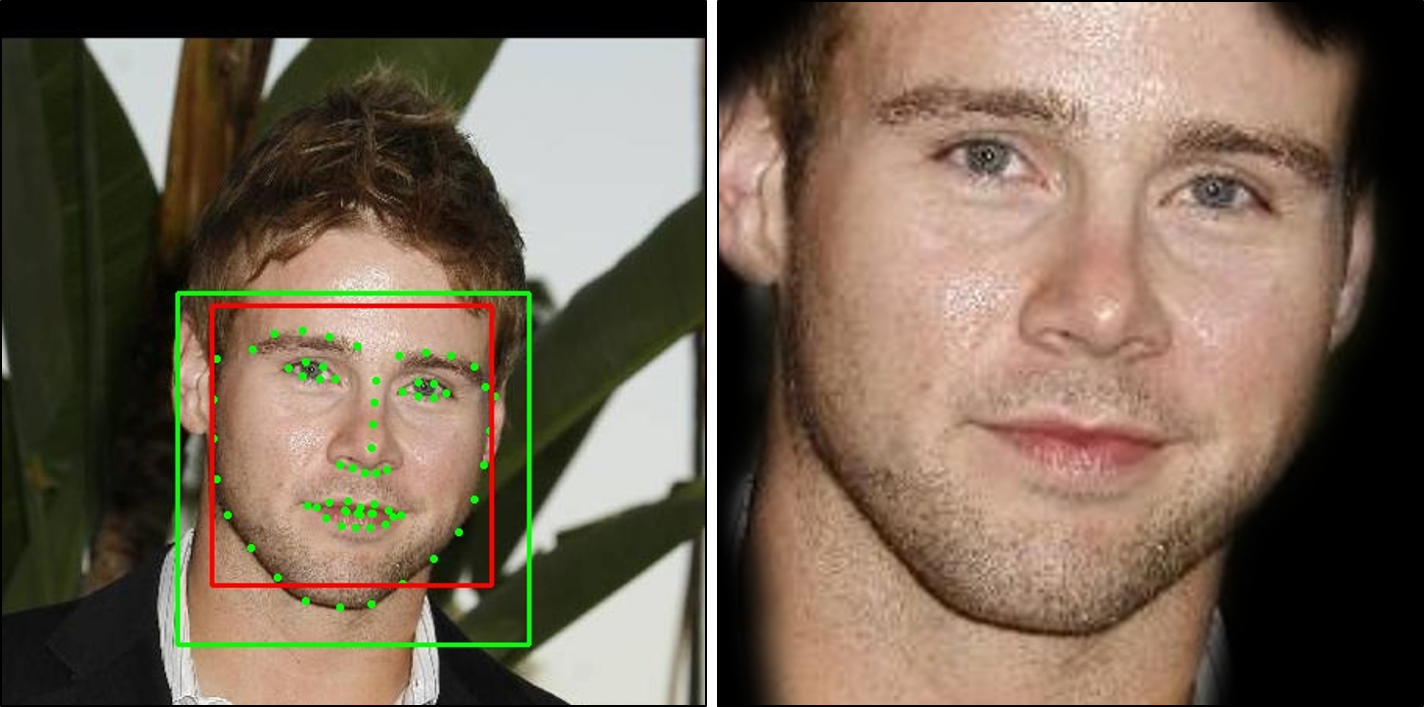
\includegraphics[width=0.22\textwidth]{figures/estimation/frontface.png} 
	}
	\subfigure[Side face]{
		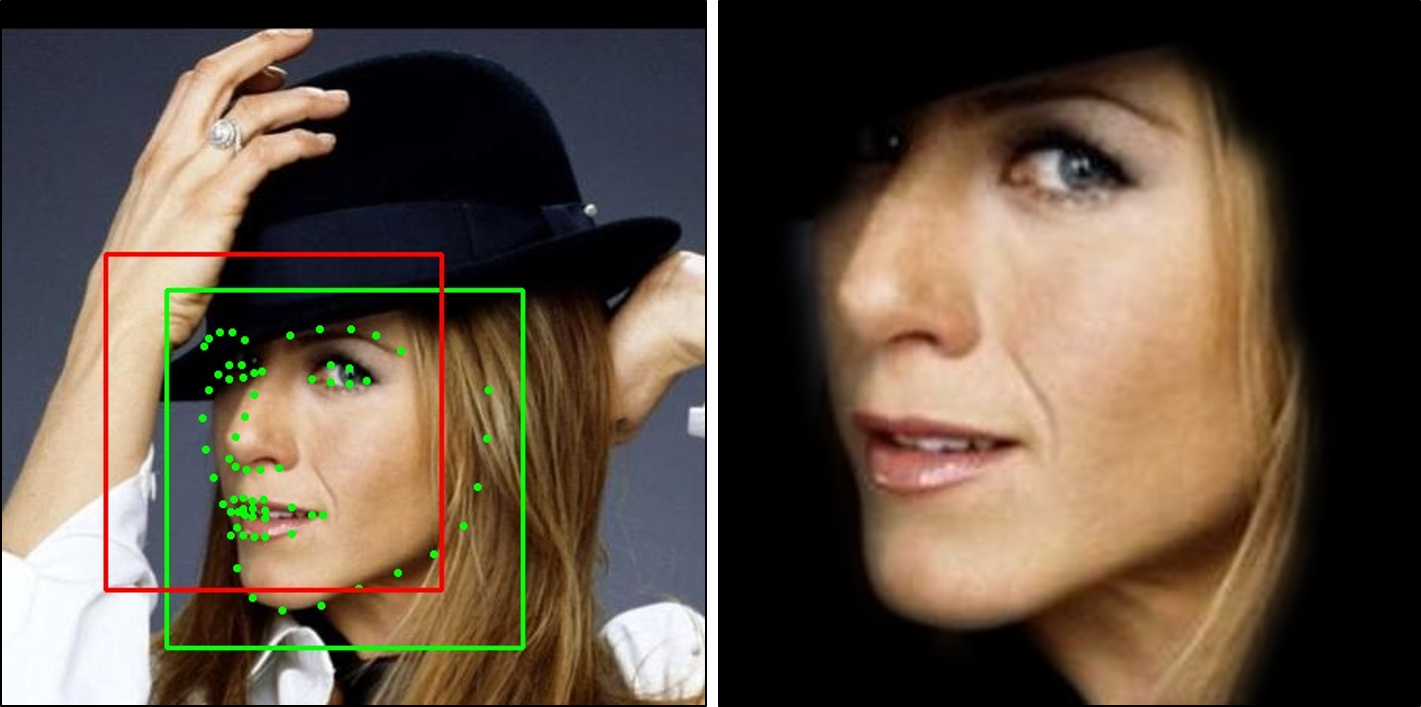
\includegraphics[width=0.22\textwidth]{figures/estimation/sideface.png} 
	}
	\vspace{-0.1in}
	\caption{Face region extraction from the photo of victims. (a) is an example of front-face, (b) is an example of side-face. The green points are the 68 feature landmark points. The red and green bounding-boxes represent the face region detected by Dlib and our method respectively.}
	\label{face_extraction}
	\vspace{-0.15in}
\end{figure}

\subsection{Depth Estimation}
To spoof 3D face authentication systems using a  public photo, we first estimate and reconstruct a depth image of the victim from his 2D photo. In general, the depth estimation has two steps: (1) Face extraction that extracts the victim's face region from his/her 2D photo to eliminate the influence of background elements, and (2) Depth estimation that estimates the depth information of the face region and generates a pixel-to-pixel depth image by using a CNN model.

\subsubsection{Face Extraction}
To estimate user depth information via a public photo, we first  detect and crop the face region to  improve the processing efficiency.

\textbf{Face Detection.} For face detection, a commonly-used  tool is the Dlib Library~\cite{dlib09}. However, using this tool alone cannot detect the  face region completely, especially the side one, as shown in the red bounding box in Fig.~\ref{face_extraction}.
To obtain the face region precisely, we improve the face detection function in the  Dlib Library by considering the following two aspects: (1) the size of the bounding box shall be appropriate to contain the entire face including the contours, and (2) the face shall  locate at the center of the bounding box to reduce background elements. To achieve it, we first utilize the shape predictor of the Dlib Library to landmark 68 key feature points of the face. Then, we use these feature points to determine the  coordinates of the center point and the side length of the bounding box such that the face can be entirely contained and located in the center of the bounding box. 
%In addition, we enlarge the bounding box with $1.2\times$ to cover the whole face region.

As shown in Fig.~\ref{face_extraction},  our face detection method can extract the face region precisely and completely for both front and side face images.

\textbf{Face Region Cropping.} 
After extracting the face region from the victim's photo, we crop and resize it to 224 $\times$ 224 pixels, i.e., the default input size for the following depth estimation model.
%To further remove the background elements, we extract the precise face region by utilizing a face segmentation method ~\cite{nirkin2018_faceswap}. 

\subsubsection{CNN-based Face Depth Estimation}
To estimate the depth information from the cropped face region, we then propose a pixel-to-pixel method based on convolution neural networks (CNNs). We employs the UNet~\cite{ronneberger2015u} as our model architecture. It uses the  ResNet-50~\cite{he2016deep} as the encoder to reduce a 224 $\times$ 224 input image into a 7 $\times$ 7 embedding feature map, and uses a decoder formed by 5 transposed convolutional layers and 10 convolutional layers to reconstruct the feature map into a 224 $\times$ 224 depth image, where each pixel represents the absolute value of the depth.  Then, we design the loss function to optimize the aforementioned estimation process.


\begin{figure}[!t]
	\centering
	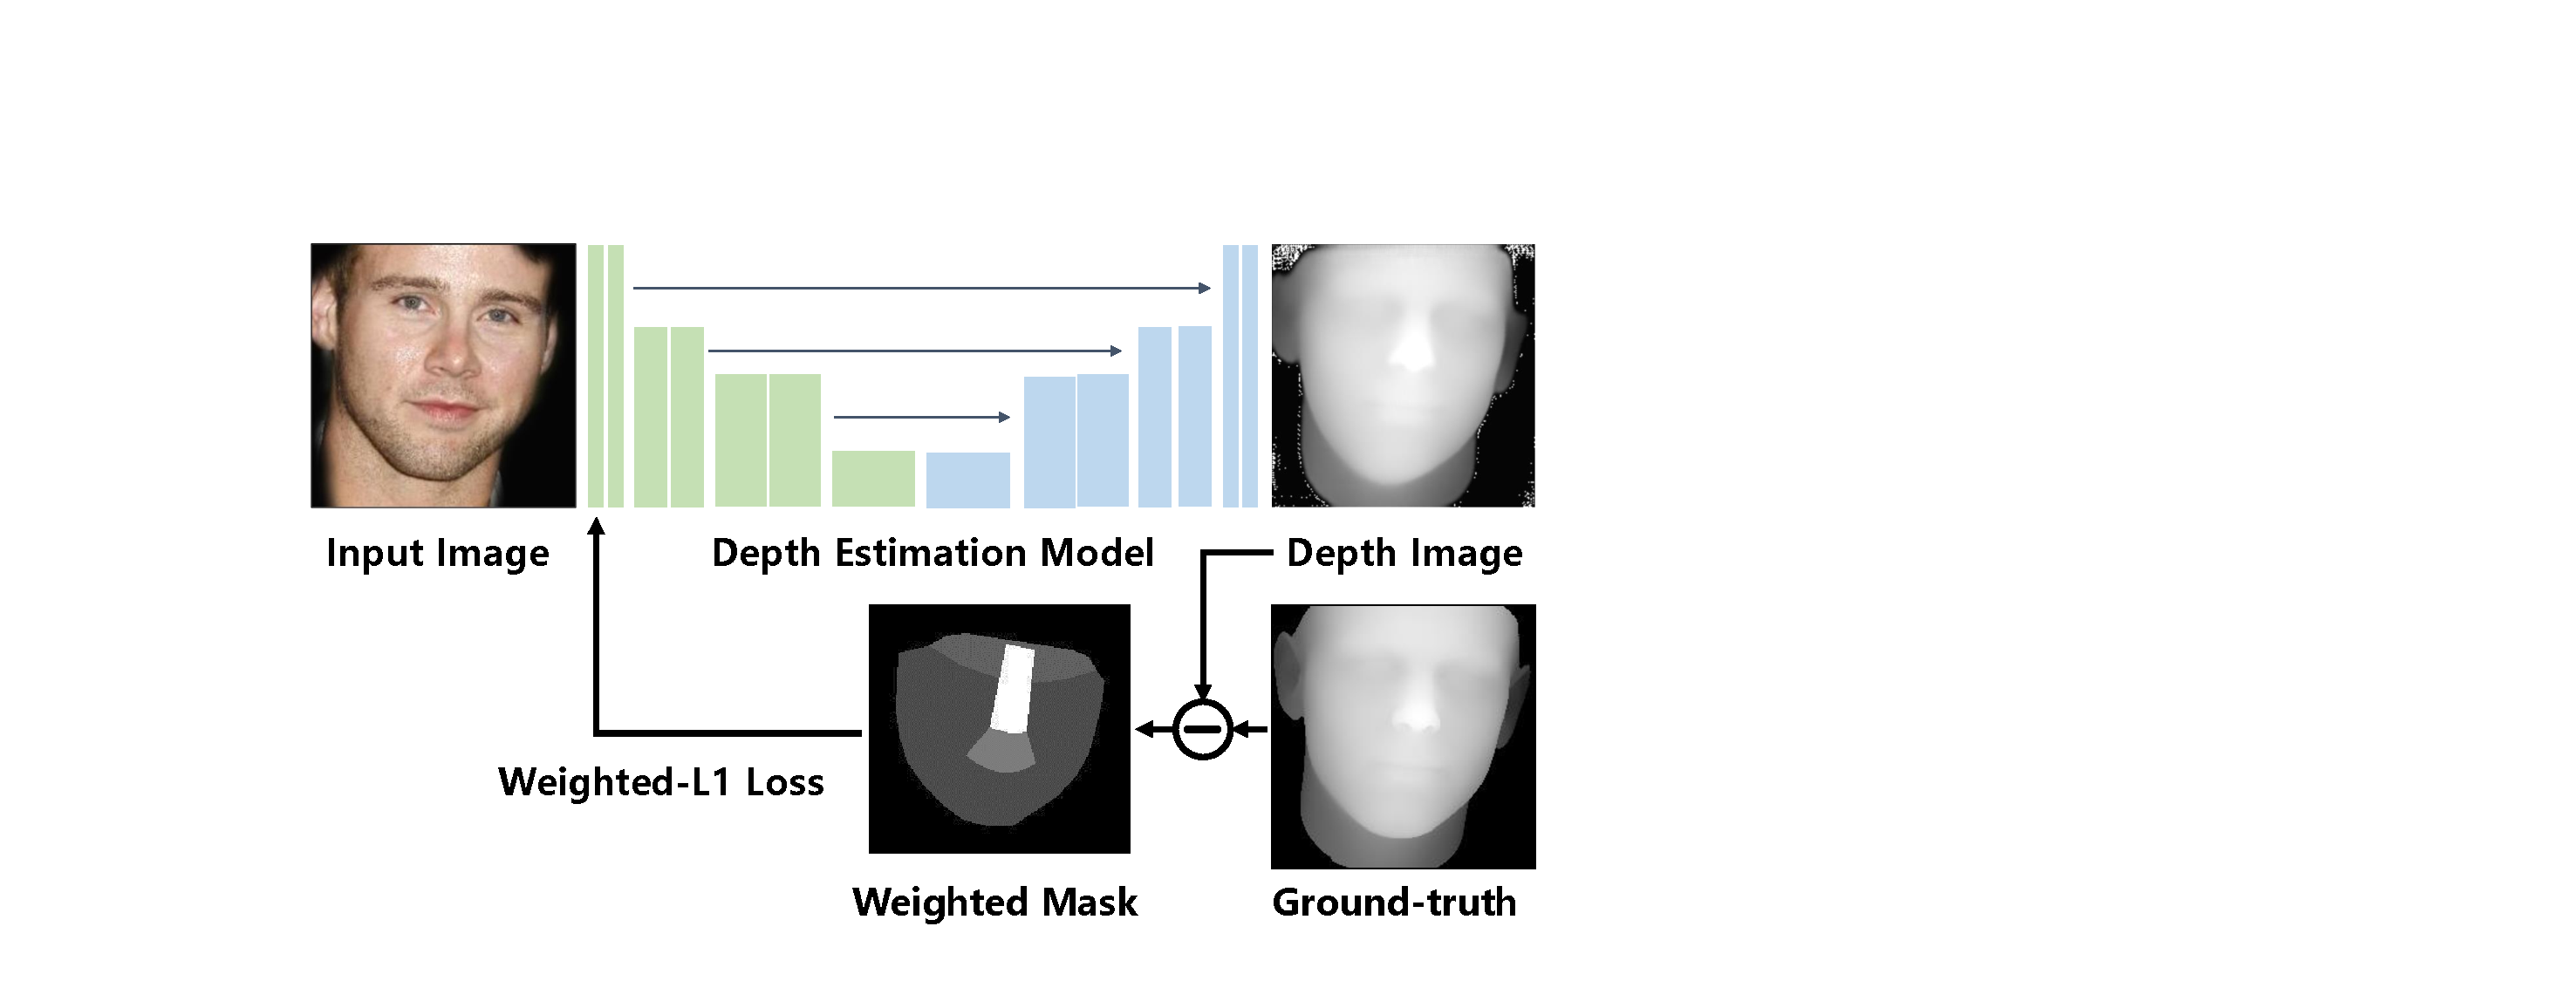
\includegraphics[width=0.47\textwidth]{figures/model_architecture_1.pdf} 
	\vspace{-0.15in}
	\caption{Model architecture for depth estimation. Images from left to right are the target image, the architecture of model and the depth image estimated by the model.}
	\label{model_architecture}
	\vspace{-0.15in}
\end{figure}

\textbf{Loss Function Design.} In general, U-Net utilizes the L1 Loss as the loss function to optimize the depth estimation task. However, the L1 Loss treats all pixels in the image equally, leading to depth estimation errors in  regions such as  noses, eyes and mouths. Those regions, however, are important in feature representation and depth reconstruction.  To address it, we propose to employ a weighted L1 Loss, which assigns more weights to the central parts of the face (i.e., the nose, eyes and mouth) compared with other regions. Specifically,  we use the landmark feature points to locate the key regions and assign different weights to them to form a weight mask. As shown in Fig.~\ref{model_architecture},  we assign a weight of  2 for the nose region, 1.5 for the eye and mouth regions, 1 for other face regions, and 0 for non-face regions. In this way, we make the model pay more attention to reconstructing the depth of the nose, eyes and mouth regions. 
The proposed weighted L1 Loss is as follows:
\begin{equation}
	Weight{-}L1=\frac{1}{N}\sum_{i=1}^{N} \lvert y_i - f(x_i) \rvert \times WeightMask
	\label{weigted_loss}
\end{equation}
where $x$ and $y$ are the input image and the ground-truth depth image,  and$f(\cdot)$ is the depth estimation model.

\textbf{Model Training.}
We use the 300W-3D face dataset~\cite{zhu2016face} as the training dataset, use the Texas 3DFR dataset~\cite{gupta2010anthropometric, gupta2010texas} as the testing dataset, and employ Adam with a learning rate of $1e{-}5$  as the optimizer to train the depth estimation model.  An illustration of the depth estimation result is shown in Fig.~\ref{estimation_result}. Compared to the ground-truth image and its 3D mesh plot, the depth image estimated from the 2D image shows a normalized mean error less than $2\%$, and can spoof the depth-based liveness detection module in commercial face authentication SDKs (i.e., Tencent, Baidu, and 3DiVi) with nearly $100\%$ attack success rates.
%We also leverage the estimated depth images into the liveness detection module in commercial face authentication SDKs (i.e., Tencent, Baidu, and 3DiVi) and get both $100\%$ attack success rates in the testing dataset.

%At training phase, we use the 300W-3D face dataset~\cite{zhu2016face} which contains images of different genders, human races, lighting conditions, and face angles as our training dataset. As for the testing dataset, we choose the Texas 3DFR dataset~\cite{gupta2010anthropometric, gupta2010texas} whose ground-truth depth images are captured by depth sensors in the real world. Before training, we pre-process the images in the dataset using the face extraction method, and ensure that the input images have removed the background noises. During training, we use Adam as the optimizer with a learning rate at $1e{-}5$ and train the model in an NVIDIA 2080 Ti GPU. Besides, we evaluate the model after each training epoch by employing Normalized Mean Error (NME) in the testing dataset and choose the model that has the best performance as our depth estimation model.

%An example of the results using our depth estimation method is shown in Fig.~\ref{estimation_result}. Compared to the ground-truth image and its 3D mesh plot, our method can successfully reconstruct the depth information from the target 2D image with a minimal error. 
%To evaluate the effectiveness of our depth estimation method within the different individuals, we conduct experiments on our testing dataset which contains 105 individuals with different gender, ethnicity, and facial expression. We achieve the result of $1.90\%$ as evaluate metric NME in the testing dataset. It is better than other face reconstruction methods such as PRNet which gets $5.51\%$ of NME in the same testing dataset. The reason is that such methods rely on the 3D Morphable Model (3DMM) to reconstruct the face, but the output images are all normalized in the 3DMM parameter space and do not accurately represent the true depth information of the face.



\begin{figure}[!t]
	\centering
	\subfigure[Ground truth]{
		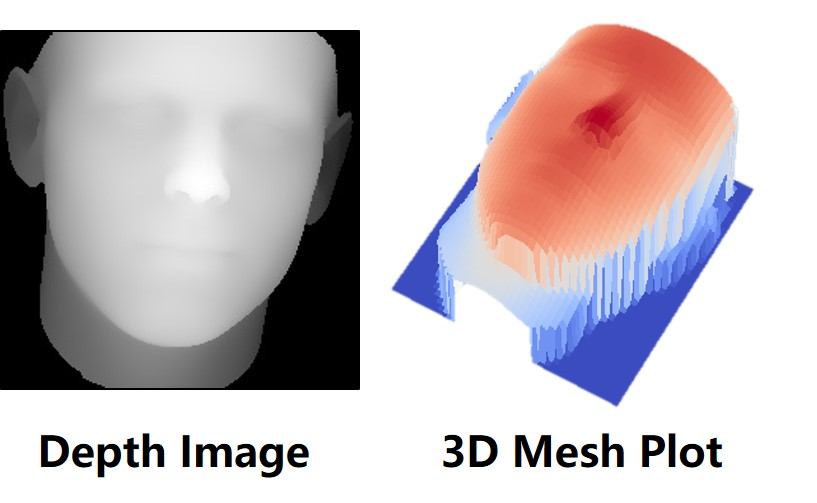
\includegraphics[width=0.22\textwidth]{figures/estimation/pred_results_groundtruth.jpg} 
	}
	\subfigure[Estimation result]{
		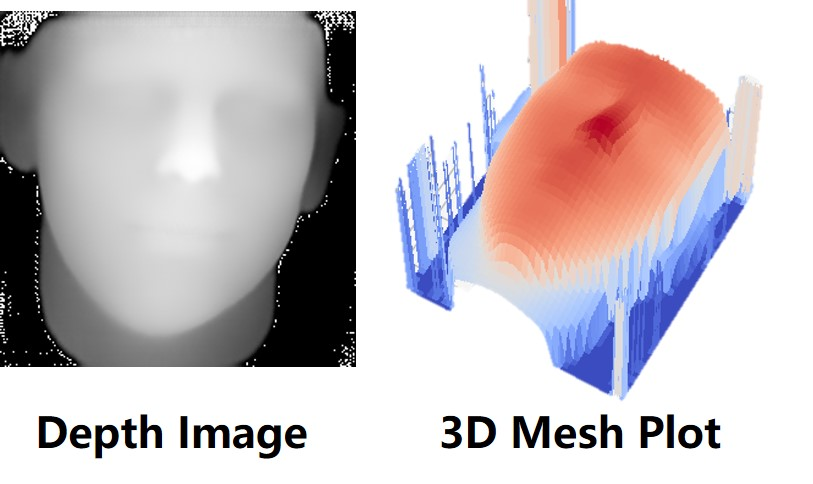
\includegraphics[width=0.22\textwidth]{figures/estimation/pred_results_pred.jpg} 
	}
	\vspace{-0.1in}
	\caption{Depth estimation results. (a) is the ground-truth depth image and its 3D mesh plot of the target image. (b) is the estimated depth image and its 3D mesh plot from our model.}
	\label{estimation_result}
\vspace{-0.15in}
\end{figure}

\subsection{Depth Forgery}
The structured-light depth camera calculates the depth information by measuring the displacements of scatter points between the template scatter pattern and the reflected one.  To spoof it, the adversary shall modulate the estimated depth information into the template scatter pattern such that it can be captured and accepted by the depth camera.  
To achieve it, we propose a depth forgery method consisting of two steps: (1) extracting the template scatter pattern of the victim camera, and (2) modulating the estimated depth image into the template scatter pattern to form the spoofing scatter pattern. 
%For a real-world attacker, she need to deploy the depth image in the physical world. Thus, we propose a depth forgery method based on the imaging mechanism of structured light camera, which consists of three steps: (1) extracting the template scatter of the camera, (2) mapping the estimated depth image into the scatter pattern and projecting the scatter pattern and ensure it can be captured by camera to form the forgery depth image we designed. In the following, we introduce our depth forgery method in detail.

\subsubsection{Template Scatter Extraction}
Different structured light depth cameras use different template scatter patterns. Thus, we shall first obtain the template scatter pattern of the victim camera. 
A naive but effective method is to use an infrared camera to capture an image towards it and extract the template scatter pattern from the captured infrared image. However, the raw infrared image usually suffers from various noises, rendering the extracted template scatter pattern not precise and thus  introducing extra errors in depth forgery. To extract a clear and precise template scatter pattern, we propose an image noise reduction method called local-threshold filtering. 

Since the scatter point is usually the brightest in its surrounding neighborhood while the noises can be dim, we can use the non-maximum suppression (NMS)~\cite{girshick2014rich} to remove the background noises. NMS is a mathematical method for picking the maximum value within an array while suppressing other values. For instance, if we have an array $S$ as $\left \{S_1, S_2, ...,S_n \right \}$ and the maximum value of $S$ is $S_{max}$, the NMS algorithm will only retain $S_k$ and set the other value to 0 as follows:
\begin{equation}
	\textbf{NMS}(S)=\left \{0, 0, ..., S_{max},...,0 \right \}\label{nms_1}
\end{equation}

To employ NMS for image processing, we extend the one-dimensional NMS into two-dimensional by using the sliding window. Specifically, we extract the pixels with the maximum grayscale value within each small region.
Since a scatter may cross more than one pixel when captured by the infrared camera, the pixels around the maximum value pixel may also have  larger grayscale values than other pixels. 
To ensure the precise of the extracted template scatter pattern, we retain the pixels whose grayscale value larger than a threshold and set the others to 0. We set the threshold dramatically with the following equation since the grayscale of the scatter points in the sliding window is related to the background brightness.
\begin{equation}
	threshold = -0.001(p_{max})^2 + 1.0001 p_{max}\label{nms_2}
\end{equation}
where $p_{max} \in \left [ 0, 255 \right ]$ is the maximum value in the sliding window. An illustration of the extracted template scatter pattern is shown in Fig.~\ref{template_extraction}.


\begin{figure}[!t]
	\centering
	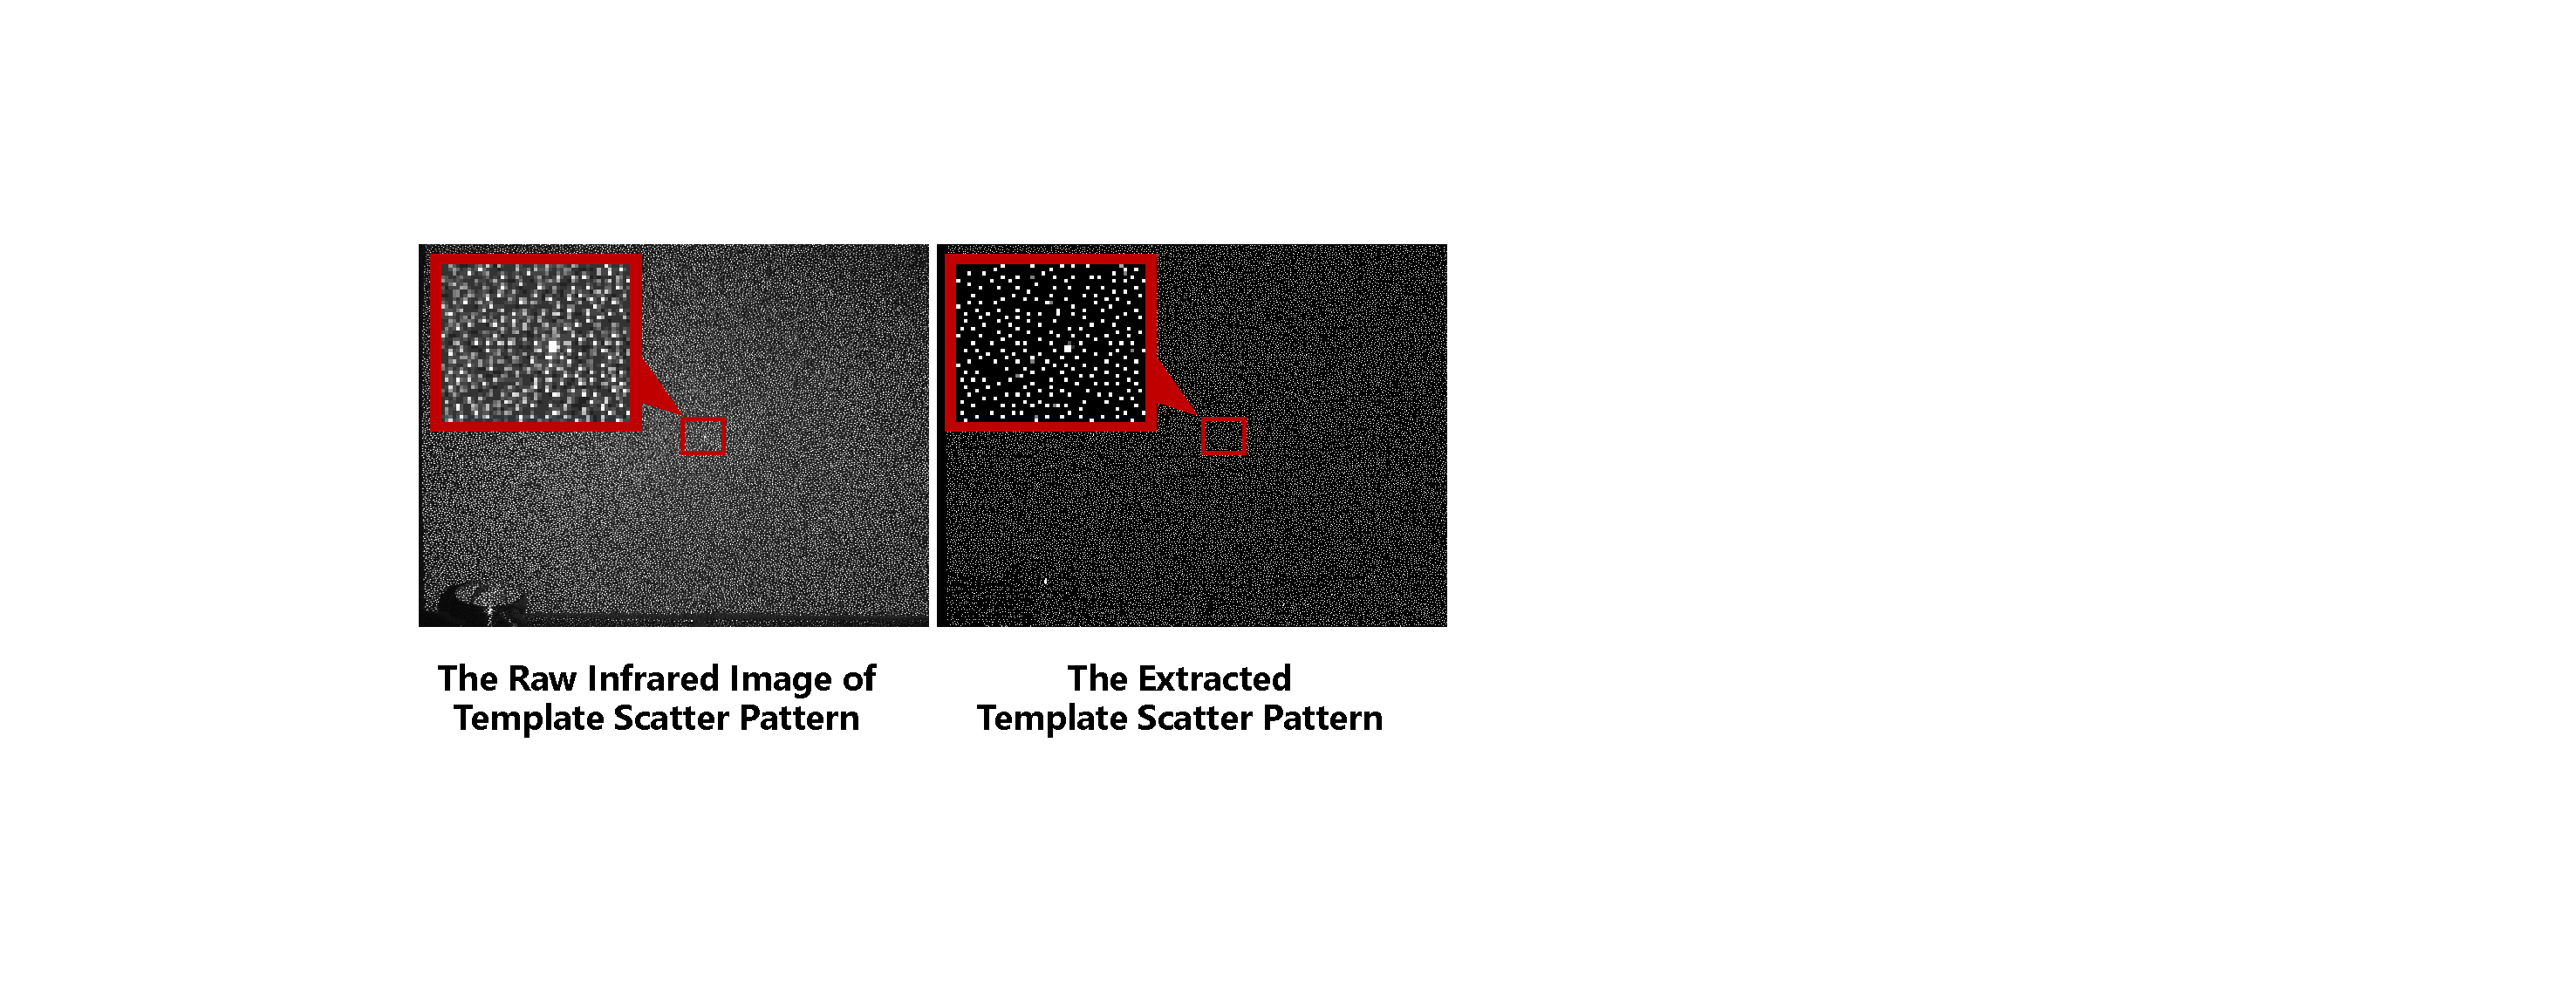
\includegraphics[width=0.48\textwidth]{figures/template_extraction.pdf} 
	\vspace{-0.15in}
	\caption{Template Extraction. Images from left to right are the raw infrared image of the template scatter pattern and the extracted template scatter pattern.}
	\label{template_extraction}
	\vspace{-0.15in}
\end{figure}


\subsubsection{Depth-to-Scatter Modulation Strategy}
Then, we modulate the estimated depth information into the extracted template scatter pattern by shifting the locations of its scatter points. 
%changing the different displacements of the scatter points on the template scatter pattern. As we have obtained the template scatter pattern and the estimated depth image, we then propose a depth-to-scatter modulation strategy to generate the diesired scatter pattern.
Two key questions here are, for each scatter point in the template: (1) What's its depth value? (2) What is  the corresponding displacement that represents the depth value?

 
%match the depth information and the template such that match each scatter point on the template  to their corresponding depth information and model the modulation process.Then, we build the mapping function from depth to scatter points' displacements, estimate its parameters and use it to generate the desired scatter pattern.

%The depth forgery in the real world rely on the desired scatter pattern. Therefore, the attacker need to transfer the digital estimated depth image into the scatter pattern, then project it and make the depth camera to capture a fake depth image. 
%To achieve such a scatter pattern from the digital depth image, we propose a depth-to-scatter mapping strategy. First, we model the depth forgery process and build the mapping function between the displacements of projected scatter points and the depths. Then, we estimate the parameters of the mapping function. Finally, we convert the whole depth image into the scatter pattern and ensure the camera can capture it to generate the forgery depth.

For the first question, we address it by coordinate alignment. We first extract the coordinates of each scatter point in the template as a set $T = \{(x_1, y_1))_ ..., (x_n, y_n)\}$. Then, based on the coordinates in $T$, we extract the corresponding depth information in the depth map as the set $D = (\delta_1, ..., \delta_n)$. 
%Each element in $T$ and $D$ represents the depth information of each scatter point.
The depth-to-scatter modulation process is then can be represented as follows:
\begin{equation}
	S = T + \Phi(D)
	\label{modulation_process}
\end{equation}
where $\Phi(\cdot)$ is the mapping function that converts the depth information to the scatter displacement, and $S$ is the desired scatter pattern.  
Thus, the key to modulate the estimated depth image into the scatter pattern is to build the mapping function $\Phi(\cdot)$. 

\textbf{Mapping Function Modeling.} 
Based on Eq.~\ref{d_cal} in Sec.~\ref{sec:background}, the structured light camera uses the reference depth $d_1$ and the displacement $\Delta x_c$ to calculate the target depth $d_2$. Thus, if a scatter point has a depth value of $d_2$, we can obtain its displacement in the camera $\Delta x_c$ as follows:
\begin{equation}
	\Delta x_c = k_cLf_c(\frac{1}{d_1} - \frac{1}{d_2}) 
	\label{d_to_xc}
\end{equation}
where $k_c$ is the number of pixels within a physical length ($1~mm$) in the camera, $L$ is the baseline distance between the camera and the projector, and $f_c$ is the focal length of the camera.

The displacement in the camera $\Delta x_c$ is then can be converted to the displacement in the projector $\Delta x_p$ as follows:
\begin{equation}
	\Delta x_p = \frac{k_pf_p}{k_cf_c}\Delta x_c 
	\label{xc_to_xp}
\end{equation}
where the $f_p$ is the focal length of the projector, and $k_p$ is the number of pixels within a physical length in the projector.

Thus, the mapping function between the depth value$d_2$ and the scatter point displacement $\Delta x_p$ can be expressed as follows:
\begin{equation}
	\Delta x_p = k_pLf_p(\frac{1}{d_1} - \frac{1}{d_2}) 
	\label{xp_to_d}
\end{equation}
Note that parameters $k_p$, $L$, and $f_p$ are related to the attack device (i.e., the infrared projector) only. Thus, the adversary does not need to know any internal parameters about the target device, making the attack more practical in the real world. 

\begin{figure}[!t]
	\centering
	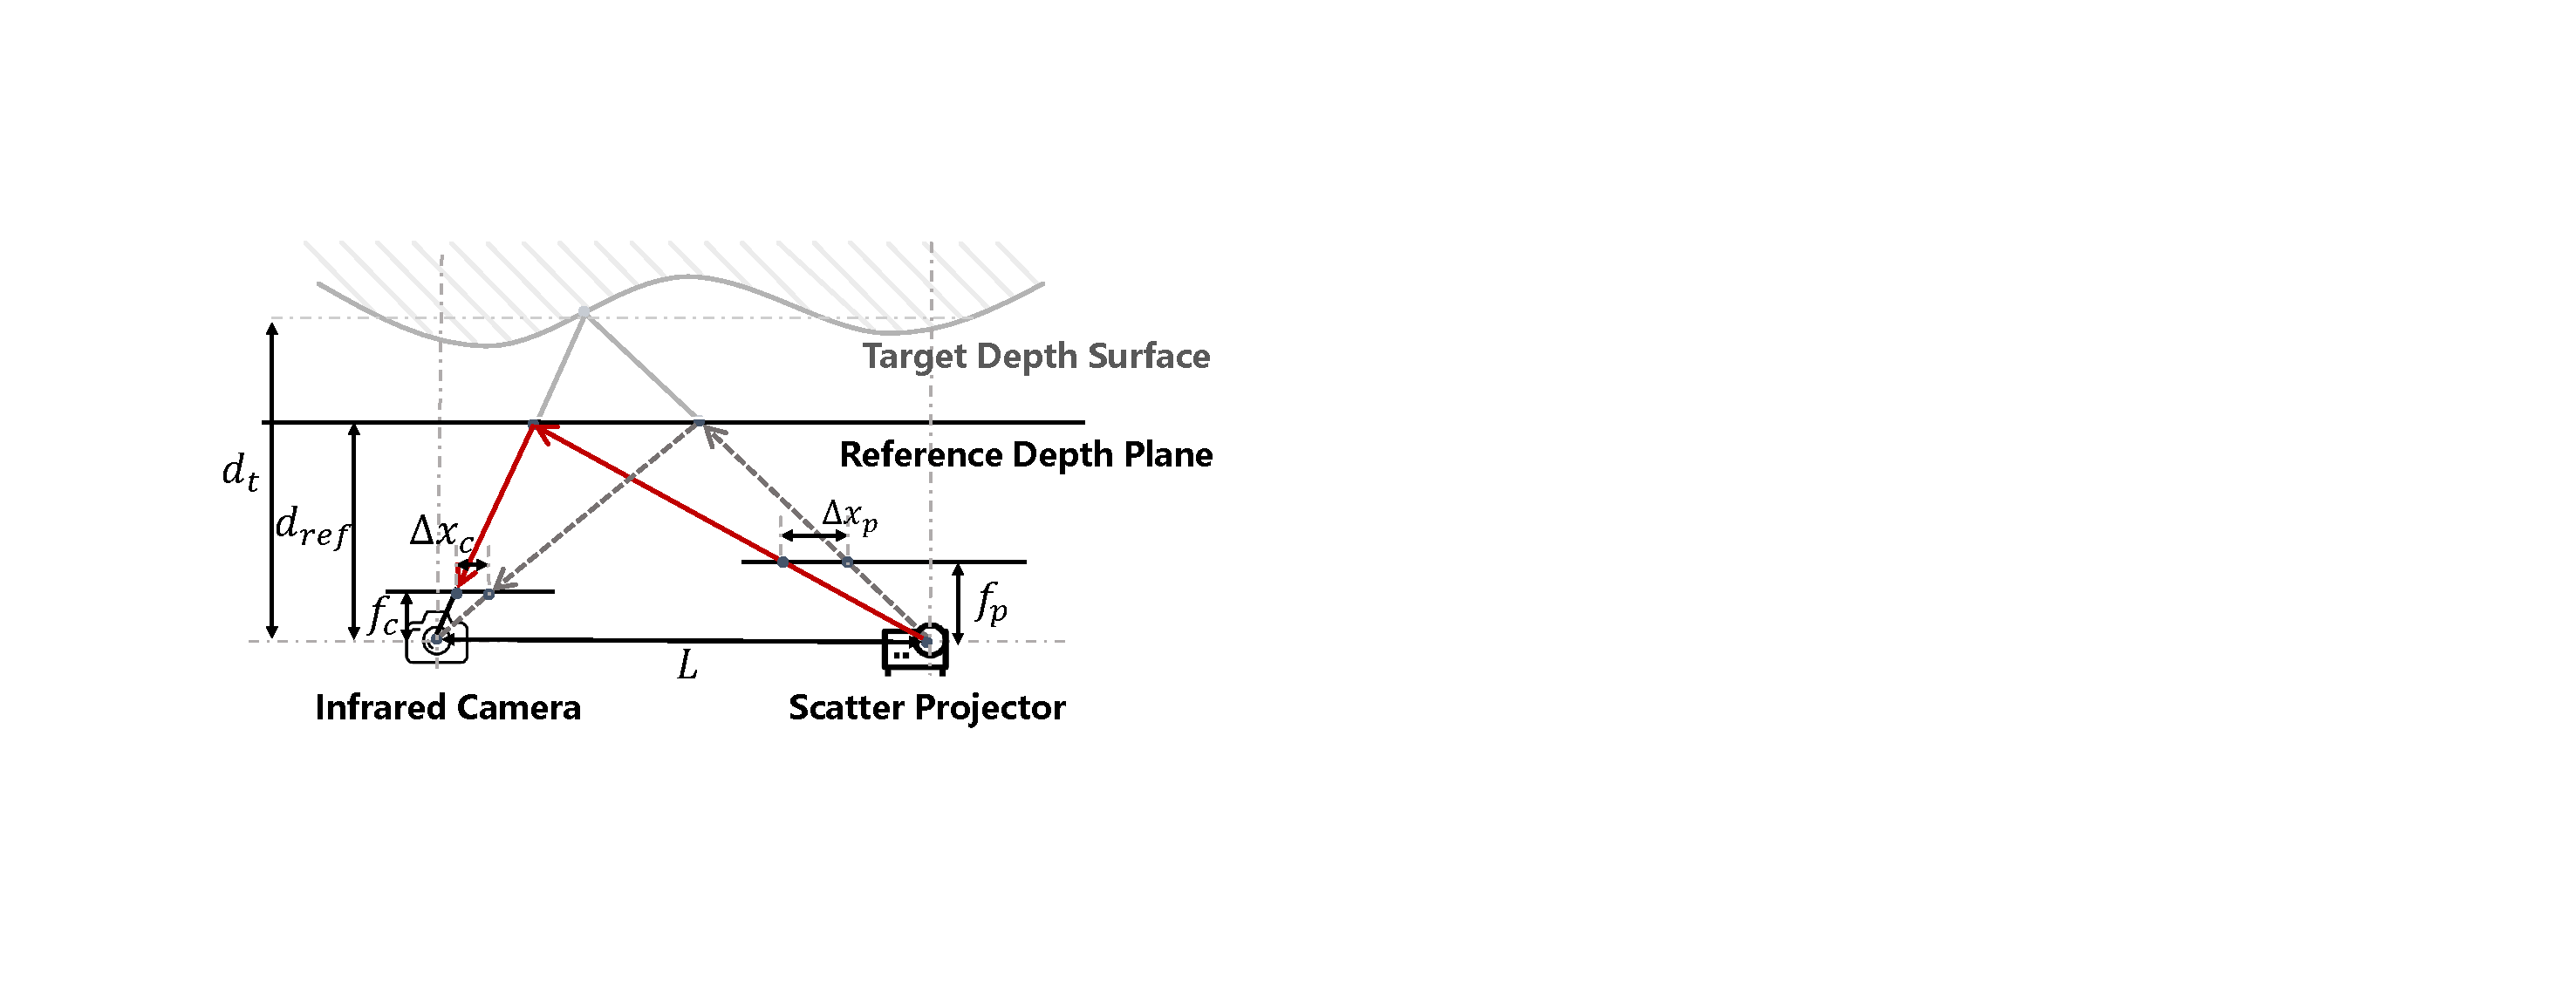
\includegraphics[width=0.475\textwidth]{figures/depth_forgery.pdf} 
	\vspace{-0.1in}
	\caption{Depth forgery. Projecting the $x_{p}^{'}$ onto the plane of depth $d_1$ and making it to be captured by camera at $x_{c2}$ on the imaging plane. The camera can be spoofed and calculate the forgery depth $d_2$.}
	\label{depth_forgery}
	\vspace{-0.15in}
\end{figure}


%As shown in Fig.~\ref{depth_forgery}, when the scatter point $p$ located at $x_p$ on the template scatter pattern is projected to the plane of the depth $d_1$, the depth camera will capture it  at $x_{c1}$. However, when we modulate $p$ into the location at $x_p'$, the depth camera then capture it at $x_{c2}$. Since the displacement of $p$ is normally caused by the change of depth, the depth camera will measure the displacements between $x_{c1}$ and $x_{c2}$ and calculate the depth of $p$ as $d_2$, which is the forgery we designed.
%
%Thus, the mapping function $\Phi(\cdot)$ should characterize the relationship between $d_2$, $x_p$ and $x_p'$.
%
%According to the similar triangles, we can derive the relation equations between $x_{p}$, $x_{p}^{'}$ and $d_2$ as follows:
%\begin{equation}
%	x_{p}^{'}=\frac{f_p}{d_1}(L-\frac{x_{c2}d_1}{f_c}) 
%	\label{xp'_cal}
%\end{equation}
%\begin{equation}
%	x_{p}=\frac{f_p}{d_2}(L-\frac{x_{c2}d_2}{f_c})  
%	\label{xp_cal}
%\end{equation}
%where the $L$ is the baseline length,  $f_p$ is the focal length of the projector, the $d_1$ is the depth of plane we project the scatter points and the $d_2$ is the target forgery depth. Based on them, we can get the mapping function as follows:
%\begin{equation}
%	\Phi (d_2) = x_p' - x_p = k_pLf_p(\frac{1}{d_1} - \frac{1}{d_2}) 
%	\label{d_cal2}
%\end{equation}


\textbf{Parameter Estimation.} 
Among the above three parameters, the baseline length $L$ and the focal length of the projector $f_p$ can be measured directly while the number of pixels within a physical length ($k_p$)  cannot.
To address it, we take $k_pLf_p$  as a joint parameter and estimate it integrally.
We record the scatter patterns on planes at depths of $1000mm$, $900mm$, and $800mm$, and use the displacements between them to determine the joint parameter. Specifically, we use the $10 \times 10$ pixels region on the center of the $1000mm$ depth plane as the template scatter pattern. Then, we use the Peak Singal-to-Noise Ratio (PSNR) as a matching function to search for the region with the highest match score and measure the displacement between them. Based on the displacements in different depths, we can estimate the joint parameter $k_pLf_p$. 
For an instance, in this paper, we use a baseline length $L$ of $20mm$, and a reference depth of $1000mm$. By measuring the displacements in depths of $1000mm$, $900mm$, and $800mm$, we can estimate the joint parameter $k_pLf_p$ as 4400 and obtain the mapping function $\Phi(\cdot)$ as follows:
\begin{equation}
		\Phi(d) = 4400 (\frac{1}{1000} - \frac{1}{d}) 
	\label{d_cal3}
\end{equation}
where the $d$ is the target depth.
By modulating the depth information of each scatter point in the set $T$, we can obtain the desired scatter pattern $S$, as shown in Fig.~\ref{depth_mapping}.
%Then, the depth camera can capture this scatter pattern and generate the corresponding forged depth image.

\subsubsection{Projection Correction}
When projecting the forged scatter pattern in practice, there can be a physical distance $L$ between the projector and the victim depth camera, causing projection distortion on the captured scatter pattern. To address it, we employ the perspective transformation before projecting, which is commonly used for image correction in computer vision. Based on the perspective transformation function shown in Eq.~\ref{align_2}, we capture both the origin and distorted scatter patterns, select four vertices of the face bounding box as the reference points, and compute the parameter matrix by comparing the pixel offsets between each pair of the vertices.
\begin{equation}
	\begin{bmatrix} \tilde{x} & \tilde{y} & \tilde{w}\end{bmatrix} = \begin{bmatrix} x&y&w\end{bmatrix}
	\begin{bmatrix} 
		a_{11}&a_{11}&a_{11} \\
		a_{21}&a_{22}&a_{23} \\
		a_{31}&a_{32}&a_{33} 
	\end{bmatrix}
	\label{align_2}
\end{equation}
where ($x$, $y$) is the point in the original image, and $w = 1$. 
Then, we use Eq.~\ref{align_3} to compensate for the origin scatter pattern to ensure the captured one is not distorted.
\begin{equation}
	x^{'} = \frac{\tilde{x}}{\tilde{w}};
	y^{'} = \frac{\tilde{y}}{\tilde{w}}
	\label{align_3}
\end{equation}

%\textbf{Depth-to-Scatter Mapping.} To convert the whole depth image, we first match the depth image to each scatter point , and then calculate their displacements to produce the desired scatter pattern. Specifically, we align the template scatter and the depth image according to the coordinates and find the depth infromation of each scatter point. Then, we apply the mapping function to calculate the displacement of each scatter point.  By shifing each scatter point, we can encode the depth information into the scatter patter.
%
%The process of depth-to-scatter mapping is shown in Fig~\ref{depth_mapping}. Afterwards, we project the desired scatter pattern to the plane of depth $d_1$ to make the depth camera capture it and generate the forgery depth image.


%find the corresponding depth information on the depth image based on the coordinates of each scatter point on the template scatter to get the following list:
%match the pixels' depth information with the scatter points on the the template scatter pattern as follows:
%\begin{equation}
%	\{(s^1, d^1, (x^1, y^1)), ...(s^i, d^i, (x^i, y^i)), ...\}
%	\label{d_match}
%\end{equation}
%where the tuple $(s^i, d^i, (x^i, y^i))$ represents the depth and coordinate position of the scatter point $i$.
%Then, we use the mapping function Eq.~\ref{d_cal2} to calculate the displacement of each scatter point and get the following list:
%\begin{equation}
%	\{(s^1, d^1, (x^{'1}, y^1)), ...(s^i, d^i, (x^{'i}, y^i)), ...\}
%	\label{d_match_2}
%\end{equation}
%where the $(x^{'i}, y^i)$ is the scatter position after mapping. Thus, based on the position of each scatter point, we can obtain the desired scatter pattern.



\begin{figure}[!t]
	\centering
	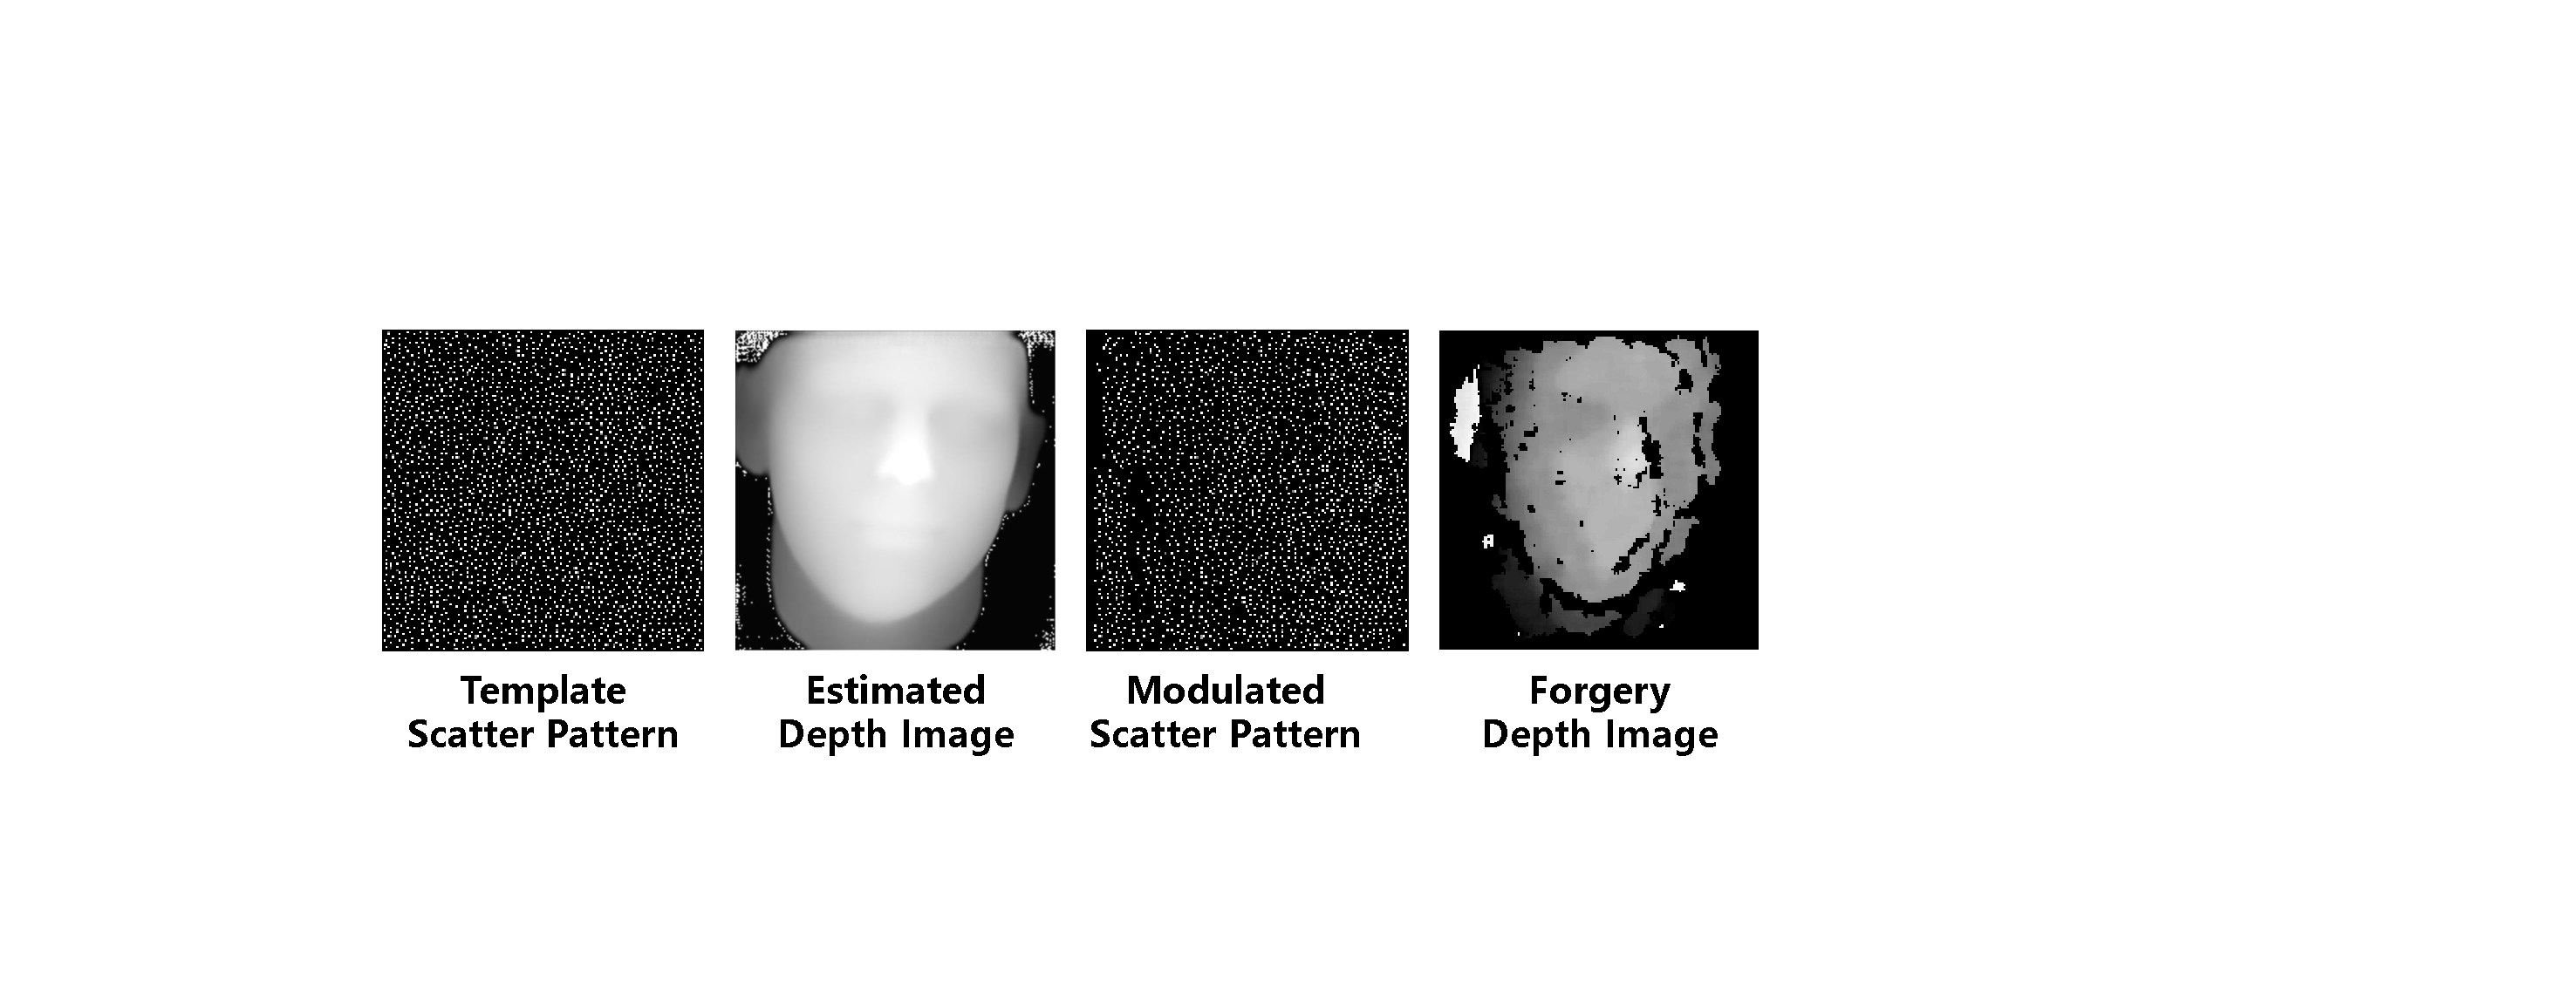
\includegraphics[width=0.48\textwidth]{figures/depth_mapping_1.pdf} 
	\vspace{-0.15in}
	\caption{Depth-to-Scatter Mapping. The digital depth image use the mapping function to convert into a crafted-design scatter pattern, then captured by the depth camera as a physical forgery depth image.}
	\label{depth_mapping}
	\vspace{-0.15in}
\end{figure}


\subsection{RGB-D Alignment}
With the above two attack building blocks, we can spoof depth-based liveness detection. However, some commercial systems may use both RGB and depth for liveness detection. In this case, we shall spoof the RGB-based liveness detection in addition to conducting the depth forgery attack. To achieve this, we propose a black-box optimization algorithm to generate  RGB adversarial examples. Then, we print  and  align it with the forged scatter pattern to launch an uniform RGB-D attack. 
%After depth forgery, we have been able to successfully spoof the 3D liveness detection module in the face authentication system. However, the liveness detection used in commercial products or services extend the 3D liveness detection to RGB-D mode for more security purposes. The reason is that RGB image can provide more color and texture information, and it can help to prevent some simple 3D replay attacks like 3D mask and dummy. Therefore, when the victim face authentication system extend to RGB-D mode, we need to synchronize the RGB attack with the aforementioned depth forgery attack. To achieve this, we first propose a RGB adversarial attack which use the black-box adversarial optimization algorithm and color calibration to generate physical adversarial examples. Then, we align the printed RGB adversarial example with the depth forgery scatter pattern physically to launch a RGB-D synchronized attack.

\begin{figure}[!t]
	\centering
	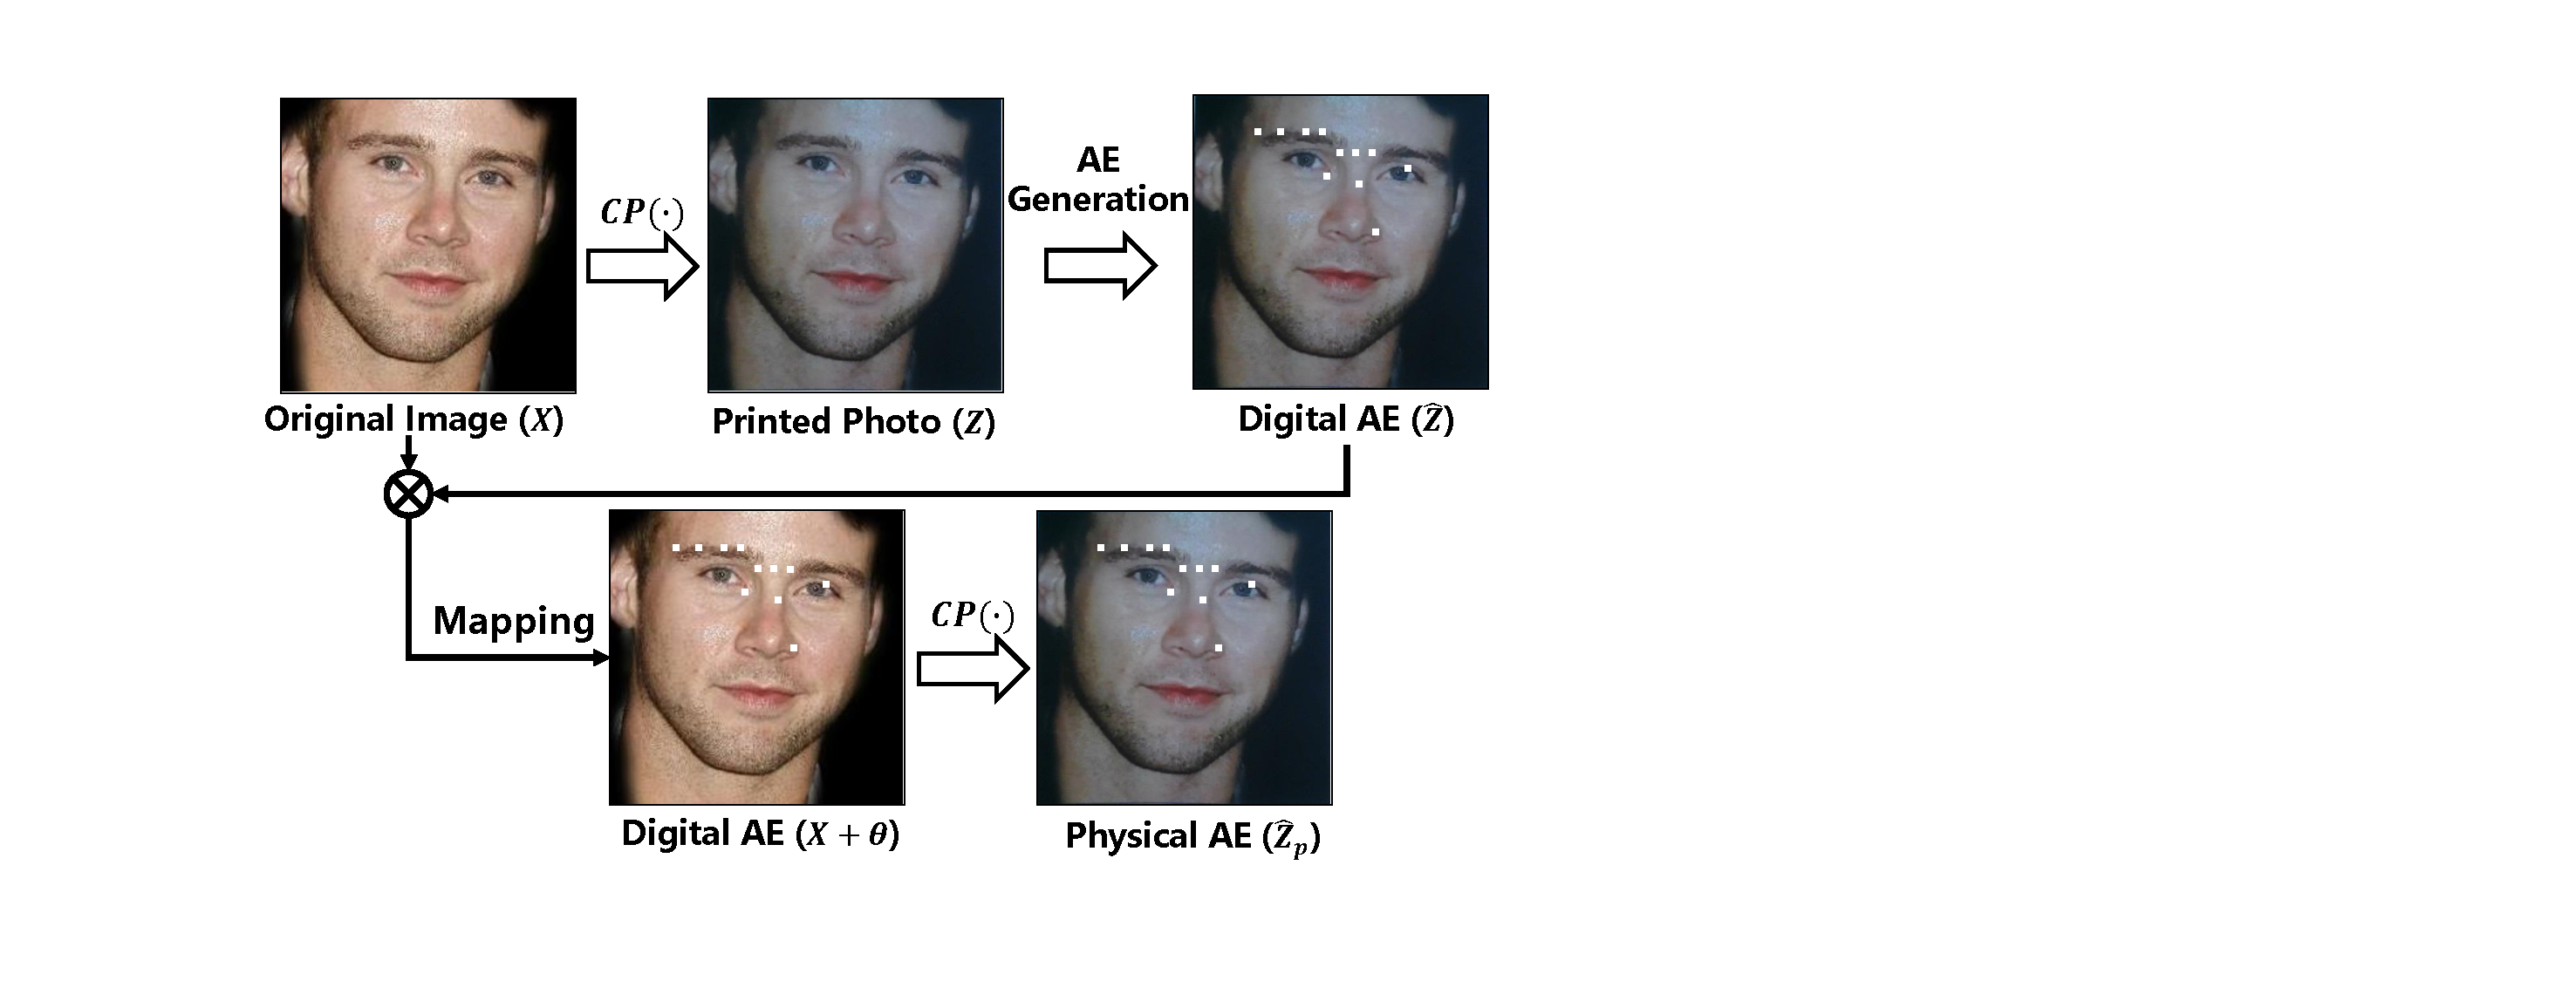
\includegraphics[width=0.45\textwidth]{figures/adv_mapping.pdf} 
	\vspace{-0.1in}
	\caption{The adversarial perturbation $\theta$ generated based on the printed photo $Z$ is applied to the original image $X$ to form the digital adversarial example $\widehat{Z}$, which is then printed and captured as the physical adversarial photo $\widehat{Z}_p$.}
	\label{rgb_mapping}
	\vspace{-0.15in}
\end{figure}

\subsubsection{RGB Adversarial Attack}
As the RGB-based liveness detection usually use CNN as its backbone, we can spoof it with adversarial examples. In general, an adversarial example in our case can be denoted as follows: 
\begin{equation}
	\widehat{Z} = Z+\theta \label{rgb_1}
\end{equation}
where $Z$ is a printed photo detected as ``non-living''  in normal circumstances,  $\theta$ is the optimized adversarial perturbation, and  $\widehat{Z}$ is the adversarial example that can successfully bypass the RGB-based liveness detection in the digital world. However, directly printing the adversarial example as
 an adversarial photo is not enough to guarantee an effective
 attack in the real world, since it suffers from color distortions
 from the printing-capturing process, resulting in a decrease
in the attack effectiveness.  To address it, we first build a printing-capturing
process model and then compensate for the color distortions
in both the printed photo $Z$ and the adversarial perturbation $\theta$.

\textbf{Color Calibration.}
To calibrate the color distortion caused by the printing-capturing process, we first build a model to describe it as follows:
\begin{equation}
	\widehat{Z}_p=C[P(Z+\theta)] =C[P(Z)]+C[P(\theta)]\label{rgb_2}
\end{equation}
where $P(\cdot)$ and $C(\cdot)$ are the abstract transfer functions without loss of generality. Since the printing-capturing process mainly processes each pixel independently~\cite{yin2013image}, we can decouple them. Based on the Eq.~\ref{rgb_2}, we can remove the effect of color distortions on the printed photo $Z$ and the adversarial perturbation $\theta$ separately.

As shown in Fig.~\ref{rgb_mapping}, since the printed photo $Z$ is the original image $X$ after a printing-capturing process, i.e., $Z=C[P(X)]$, we can replace $Z$ with the origin image $X$ in Eq.~\ref{rgb_2} to eliminate the color distortions. For the adversarial perturbation $\theta$, we use white adversarial units instead of pixel-level adversarial perturbations, since the color white does not produce color distortions under the CMYK printing mode. 
By implementing the color calibration, we can get a desired adversarial photo as follows:
\begin{equation}
	\widehat{Z}_p=C[P(X+\theta)] =C[P(X)]+C[P(\theta)]=Z+\theta\label{rgb_3}
\end{equation}

\textbf{Black-box Adversarial Example Generation.}
With the selected perturbation color and size, we then generate the adversarial perturbations $\theta$ that can bypass the RGB-based liveness detection in the digital world.
In this paper, we consider the RGB-based liveness detection to be a black-box and thus we can only get the confidence scores of the liveness detection results. As a result, we propose a query-based evolutionary strategy to generate the adversarial perturbations, as shown in Algorithm~\ref{alg1} in the Appendix.
Specifically, we use a printed photo $Z$ as the input and utilize a 2D adversarial perturbation unit with a size of $w\times h$  to scan through its face region boxed by the face authentication system. Each time after adding an adversarial perturbation unit, we get the liveness confidence score from the SDKs or APIs and retain the adversarial perturbation unit that can raise the liveness confidence score. 
Different from other black-box adversarial attacks, we do not have to consider the stealthiness of adversarial examples in this paper. As a result, we do not consider the shortest distance between the adversarial example and the original image during optimization. 

After scanning the whole face region, we extract the adversarial perturbation $\theta$ and apply it to the original image $X$ to form the digital adversarial example $\widehat{Z}$,  which is then printed and captured as the physical adversarial photo $\widehat{Z}_p$. 


\subsubsection{Face Region Alignment}
To align the RGB adversarial photo and the depth scatter pattern to ensure a uniform RGB-D attack, we localize five key face feature points (i.e., eyes, nose tip, and mouth corners) in both depth and RGB images. Then, we fix the distance between the projector and the printed RGB adversarial photo, then align the feature points by adjusting the position and angle of the photo.


%However, directly using the adversarial photo is not enough to guarantee an effective attack in the real world, since it suffers from color distortions from the printing-capturing process, resulting in a decrease in the attack effectiveness. Moreover, since we regard the RGB-D liveness detection model as a black-box, existing robustness enhancement methods such as Expectation over Transformation~\cite{athalye2018synthesizing} are not applicable. To address it, we first build a printing-capturing process model and then compensate for the color distortions in both the printed photo $Z$ and the adversarial perturbation $\delta$.

%Without loss of generality, we abstract the printing and capturing processes  as two functions $P(\cdot)$ and $C(\cdot)$. An adversarial photo $\widehat{Z}_p$ captured by the liveness detection module is actually its corresponding digital-world adversarial example $\widehat{Z}$ after a printing-capturing process. And since the printing-capturing process mainly processes each pixel independently~\cite{yin2013image}, we can express the adversarial photo $\widehat{Z}_p$ as follows: 
%\begin{equation}
%	\widehat{Z}_p=C[P(\widehat{Z})] =C[P(Z+\delta)] 
%\end{equation}
%Since the printing-capturing process mainly processes each pixel independently~\cite{yin2013image}, we can further express the adversarial photo $\widehat{Z}_p$ as follows: 
%\begin{equation}
%		\widehat{Z}_p=C[P(Z+\delta)] = C[P(Z)] + C[P(\delta)] \neq Z+\delta \label{rgb_2}
%\end{equation}
%Based on this equation, we find that the real-world adversarial photo $\widehat{Z}_p$ can be restored to the digital-world adversarial example $\widehat{Z}$ by removing the effects of printing and capturing $C[P(\cdot)]$  on the printed photo $Z$ and the adversarial perturbation $\delta$ separately.


%\begin{figure}[pt]
%	\centerline{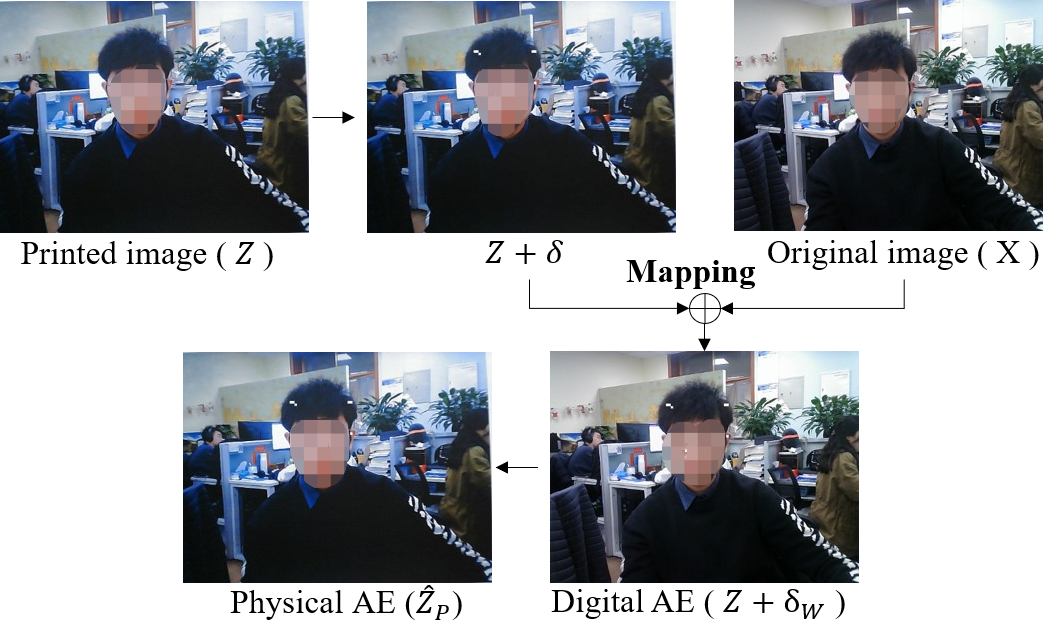
\includegraphics[width = 0.45\textwidth]{figures/adv_map.png}}
%	\vspace{-0.15in}
%	\caption{The adversarial  perturbation $\delta$ generated based on the printed photo $Z$ is applied to the original image $X$ to form the digital  adversarial example $\widehat{Z}$,  which is then printed and captured as the physical adversarial photo $\widehat{Z}_p$. }
%	\label{rgb_adv}
%		\vspace{-0.15in}
%\end{figure}

%\textbf{Printed Photo  Calibration. }
%To eliminate the color distortion on the photo part, we use the
%printed photo $Z$ for optimization but apply the generated adversarial perturbations on the original (digital) image $X$ of the printed photo $Z$ to form the adversarial example $\widehat{Z}$. The printed photo $Z$ is the original image $X$ after a printing-capturing process, i.e., $Z=C[P(X)]$. As a result, if we apply the generated adversarial perturbations on the original image $X$ instead of the printed photo $Z$, the adversarial photo $\widehat{Z}_p$ becomes as follows:
%\begin{equation}
%	\widehat{Z}_p=C[P(X+\delta)] =C[P(X)]+C[P(\delta)]= Z + C[P(\delta)]\label{rgb_3}
%\end{equation}
 %An illustration is shown in Fig.~\ref{rgb_adv}, where we first capture the legitimate user's image as $X$, and then print $X$ out as the printed photo $Z$ (detected as ``Non-living''). Then, we use the printed photo $Z$ to generate adversarial perturbations $\delta$ that can spoof the RGB-based liveness detection, apply it to the origin image $X$ to form the adversarial example $\widehat{Z}$, and  finally print it out as the physical adversarial photo $\widehat{Z}_p$. 
%In this way, we eliminate the color distortion on the photo part.


%\textbf{Perturbation Calibration.} 
%We then calibrate the impacts of printing and capturing for the adversarial perturbation $\delta$. Specifically, we consider reducing its effects from two aspects: (1) perturbation color, and (2) perturbation size. 


%Adversarial perturbations areusually of various colors, resulting in severe color distortions during the printing-captioning process. 
%Using a color that suffers from fewer color shifts in both the printing and capturing process can help enhance the robustness of the generated adversarial perturbations.
%To achieve it, we analyze the commonly-used color mode of the printer, i.e., CMYK~\cite{yin2013image}, and find that in this color mode, white  is represented as 0 cyan, 0 yellow, 0 magenta, and 0 black. As a result, using the color white to generate adversarial perturbations is likely to reduce the color distortion caused by the printing. Moreover, since the white color reflects all lights and thus may also suffer from the least distortion during the imaging process. Thus, by generating adversarial perturbations of white, we can get a desired adversarial photo as follows :

%\begin{equation}
%	\widehat{Z}_p=C[P(X+\delta)] = Z + \delta
%\end{equation}

%Despite reducing the impacts of printing and capturing by using white adversarial perturbations, increasing the size of each perturbation can also help improve its robustness in the real world.
%The reason is that pixel-level adversarial perturbations are too subtle to survive from noises introduced by the  printing-capturing process.
%As a result, we use a square instead of a pixel as the basic unit of the adversarial perturbations. Since the face authentication system allows a small portion of the user's face to be obscured, such an operation will not impact face recognition.




\section{Evaluation}

In this section, we evaluate \texttt{DepthFake} against three commercial liveness detection modules in the real world. 
We use the attack success rate (SR) as the metric to evaluate our attack, which is the ratio of the number of successful attacks against liveness detection modules over the total number of conducted attacks. 


\subsection{Experimental Setup}
\label{sec:experimental}

\begin{figure}[pt]
	\centerline{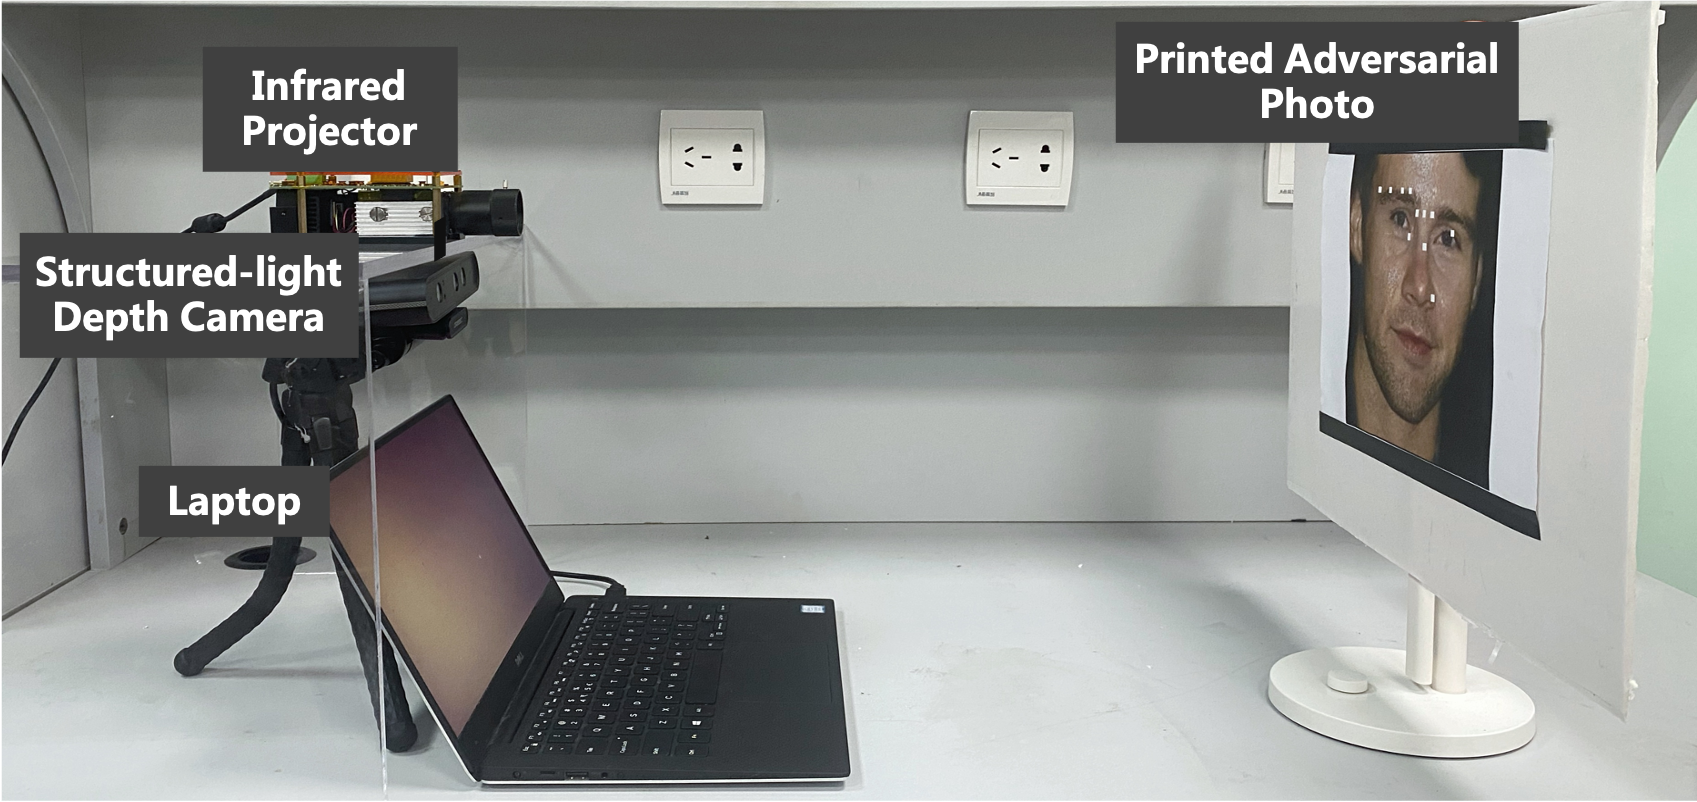
\includegraphics[width = 0.48\textwidth]{figures/setup.png}}
%	\vspace{-0.1in}
	\caption{Experimental setup. An infrared projector is used to project a structured light scatter pattern onto an adversarial photo of a legitimate user present in front of the target module to launch RGB-D attacks.}
	\vspace{-0.1in}
	\label{setup}
\end{figure}


\begin{table}[pt]
	\small 
	\caption{Default parameters during evaluation.}
	\vspace{-0.2in}
	\begin{center}
		\setlength{\tabcolsep}{1.5mm}{
			\renewcommand{\arraystretch}{1.2} 
			\begin{tabular}{c|c|c}
				\hline
				\textbf{Resolution} & \multicolumn{2}{c}{$640 \times 480$ pixels (480p)} \\
				\hline
				\multirow{2}{*}{\textbf{Light Condition}} & illumination intensity & $300~lx$ \\
				\cline{2-3}
				& color temperature & $6500~K$\\
				\hline
				\multirow{4}{*}{\textbf{Thresholds}} & Tencent Cloud & RGB: 0.4, Depth: 0.5 \\
				\cline{2-3}
				& Baidu Cloud & RGB: 0.8, Depth: 0.8 \\
				\cline{2-3}
				& 3DiVi & RGB: 0.9, Depth: 0.5 \\
				\hline
		\end{tabular}}
		\label{default_param}
	\end{center}
	\vspace{-0.15in}
\end{table}

\begin{table*}[t]
	\caption{Overall Performance of \texttt{DepthFake} attacks with four users against four different  liveness detection modules.}
	\vspace{-0.1in}
	\begin{center}
		\setlength{\tabcolsep}{6.5mm}{
			\renewcommand{\arraystretch}{1.2} 
			\begin{tabular}{c|c|c|c|c}
				\hline
				\multirow{2}{*}{\textbf{Datasets}} & \multirow{2}{*}{\textbf{Modalities}} & \multicolumn{3}{c}{\textbf{Target Systems}}                   \\
				\cline{3-5}
				& & Tencent Cloud & Baidu Cloud & 3DiVi \\
				\hline
				\hline
				\multirow{2}{*}{300W-3D} & Depth
				& \textit{74.1\%} (THR:0.4) &  \textit{68.0\%} (THR:0.8) & \textit{95.2\%} (THR:0.5) \\
				\cline{2-5}
				& RGB-D
				& \textit{49.0\%} (THR:0.4, 0.5) & \textit{45.0\%} (THR:0.8, 0.8) & \textit{71.2\%} (THR:0.9, 0.5) \\
				\hline
				\multirow{2}{*}{Texas-3DFR} & Depth
				& \textit{73.2\%} (THR:0.4) &  \textit{70.2\%} (THR:0.8) & \textit{94.3\%} (THR:0.5) \\
				\cline{2-5}
				& RGB-D
				& \textit{45.1\%} (THR:0.4, 0.5) & \textit{38.0\%} (THR:0.8, 0.8) & \textit{56.2\%} (THR:0.9, 0.5) \\
				\hline
				\multirow{2}{*}{Volunteers} & Depth
				& \textit{71.3\%} (THR:0.5) &  \textit{64.5\%} (THR:0.8) & \textit{98.5\%} (THR:0.5) \\
				\cline{2-5}
				& RGB-D
				& \textit{71.3\%} (THR:0.4, 0.5) & \textit{63.8\%} (THR:0.8, 0.8) & \textit{72.3\%} (THR:0.9, 0.5) \\
				\hline
		\end{tabular}}
		\label{overall}
	\end{center}
	\vspace{-0.1in}
\end{table*}

\textbf{Target systems.} 
We use a commercial 3D camera Orbbec Astra Pro~\cite{da2020comparison} equipped with an RGB camera and a structured light depth camera as the hardware part of our target systems, as shown in Fig.~\ref{setup}. 
%The scatter projector of the structured light depth camera can project a fixed infrared structured light scatter pattern. 
We use three commercial face authentication SDKs/APIs as the software part of the target systems and try to spoof their liveness detection modules, including (1) Tencent Cloud~\cite{tencent}, (2) Baidu Cloud~\cite{baidu}, and (3) 3DiVi Face~\cite{3divi}. We deploy these SDKs/APIs on a DELL XPS 13 laptop and acquire the liveness confidence scores by calling interfaces.

\textbf{Attack Devices.} We use an infrared projector DLP4500SL02 Evaluation Module~\cite{chong2017intraoperative} as the attack device to project the modulated structured light scatter pattern, which has a resolution of $1280 \times 800$ pixels, and a projecting image size of $270~mm \times 168~mm$.
In addition, we use a printed adversarial photo of a legitimate user placed in front of the camera to spoof the RGB-based liveness detection, as shown in Fig.~\ref{setup}.

\textbf{Default Attack Setting.} During the experiments, we put the infrared projector above the target 3D camera with a distance of $20~mm$ and fix the distance between the projector and the adversarial photo as $500~mm$.
All the adversarial photos are printed with a  size of $400~mm \times 300~mm$.
Other default settings including the camera resolution, the light condition, and the thresholds of target systems are shown in Tab.~\ref{default_param}.

%The default background illumination intensity is $400~lx$ and the color temperature is $6500~K$. The default camera resolution is 480p, i.e., $640\times480$ pixels. The default thresholds of the target systems are as follows: (1) Tencent Cloud (RGB: 0.4, RGB-D: 0.4 for RGB and 0.5 for Depth), (2) Baidu Cloud (RGB: 0.8, RGB-D: 0.8 for RGB and 0.8 for Depth), (3) ArcFace (RGB: 0.5), (4) Huawei Cloud (RGB: 0.5).

\textbf{Datasets.} We evaluate our attacks on two datasets 300W-3D~\cite{zhu2016face} and Texas-3DFR~\cite{gupta2010anthropometric, gupta2010texas}. 
The 300W-3D dataset contains more than 3800 facial images with different genders, ages, races, illumination conditions, pose, occlusion, and face sizes. 
The Texas-3DFR dataset contains 1149 pairs of facial images from 105 adults of different genders, ages, and races.
For each dataset, we select 20 images with different genders, ages, and races to launch \texttt{DepthFake}.


\textbf{Volunteers.} We recruit five volunteers including three males and two females to evaluate the effectiveness of \texttt{DepthFake} attacks in the real world, and have obtained  the approval from the Institutional Review Board (IRB).

%\begin{figure*}[h!]
%	\centering
%	\subfigure[Attack Success Rates on various light conditions.]{
%		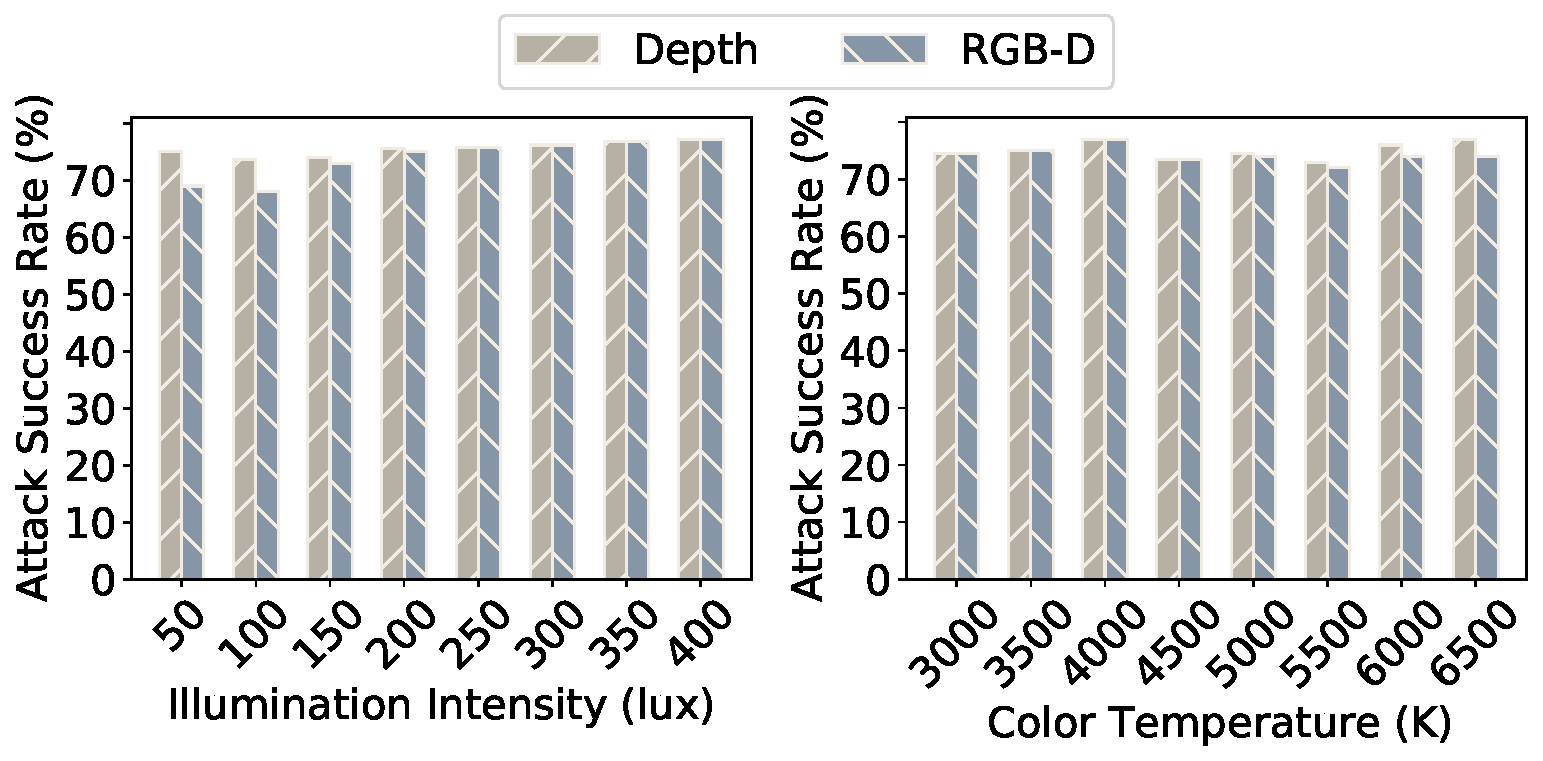
\includegraphics[width=0.48\textwidth]{figures/light_condition.pdf}
%	}
%	\subfigure[Confidence Scores on various light conditions.]{
%		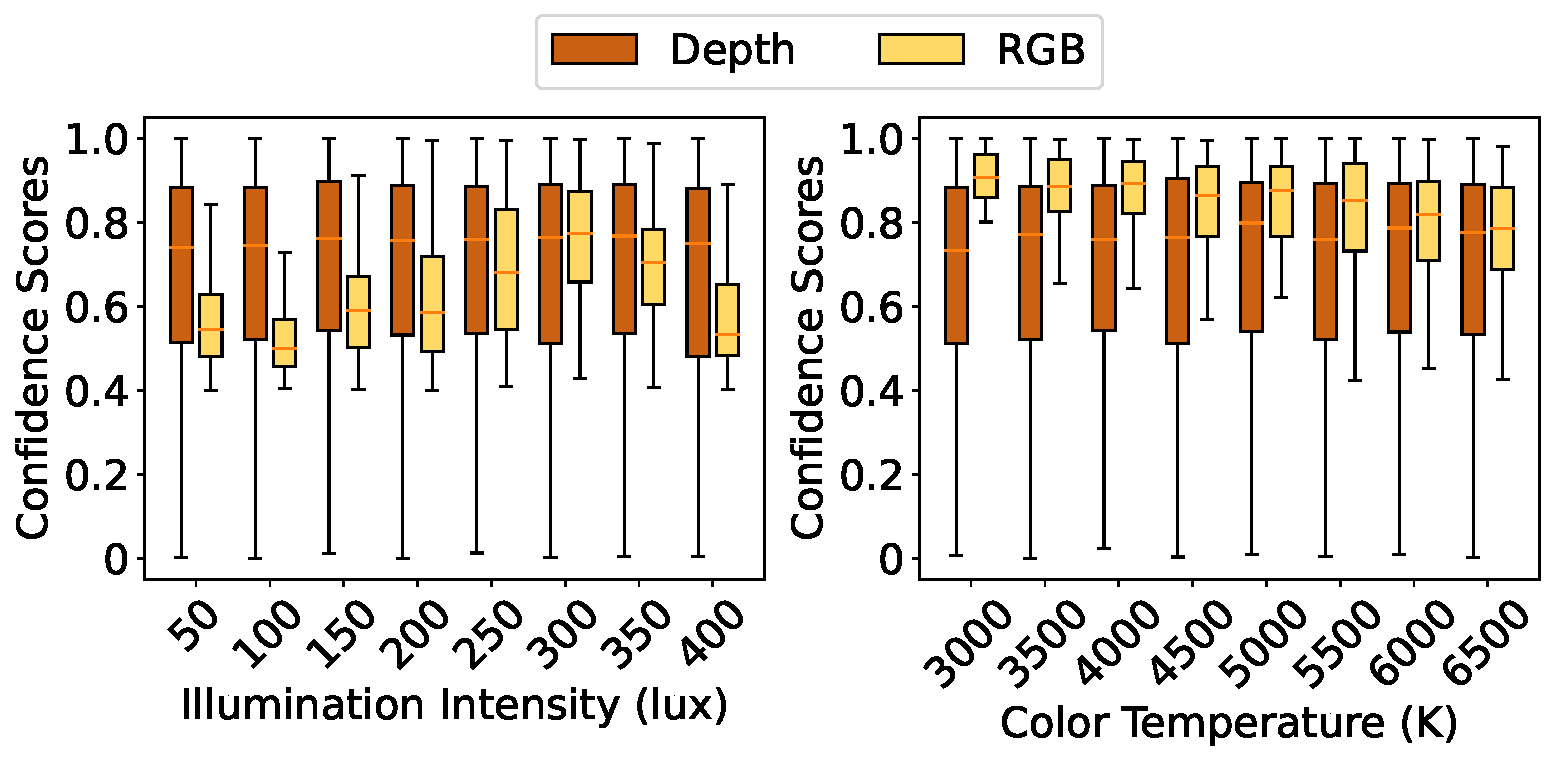
\includegraphics[width=0.48\textwidth]{figures/light_condition_scores.pdf}
%	}
%	\vspace{-0.1in}
%	\caption{Impact of \texttt{DepthFake} under various light conditions}
%	\label{light_condition}
%	\vspace{-0.1in}
%\end{figure*}

\begin{figure}[pt]
	\centerline{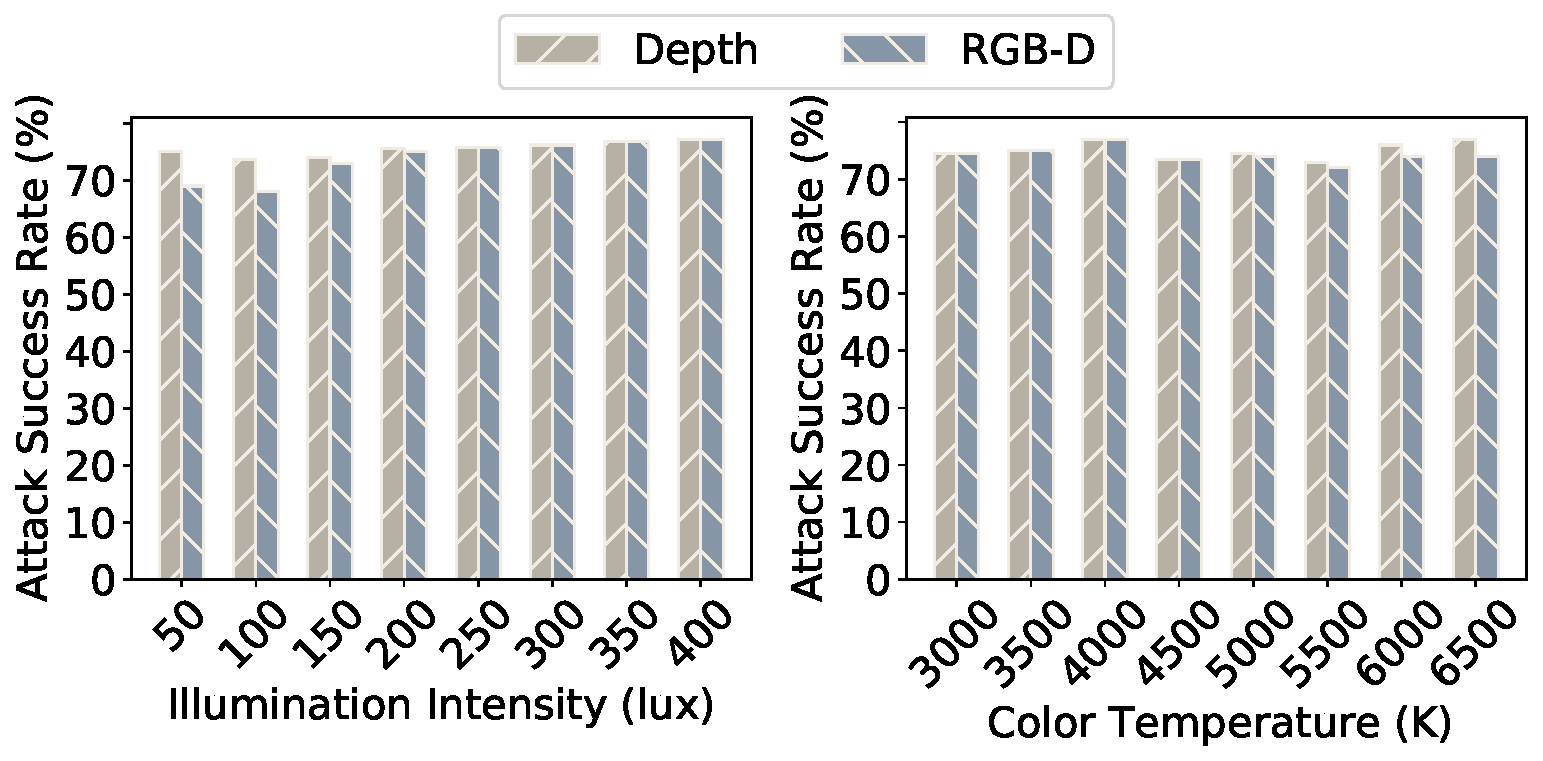
\includegraphics[width = 0.48\textwidth]{figures/light_condition.pdf}}
	\vspace{-0.15in}
	\caption{Impact of \texttt{DepthFake} attacks under various light conditions.}
	\label{light_condition}
	\vspace{-0.1in}
\end{figure}

\subsection{Overall Performance}
We first evaluate the overall performance of the Depth and RGB-D attacks on different people against three commercial liveness detection modules, i.e., Tencent Cloud, Baidu Cloud, and 3DiVi, under the default setting. 
The results shown in Tab.~\ref{overall} demonstrate that the Depth attacks can achieve an overall attack success rate of $72.8\%$ against Tencent Cloud, $67.6\%$ against Baidu Cloud, and $96\%$ against 3DiVi. The RGB-D attacks can achieve an overall attack success rate of $55.1\%$ against Tencent Cloud, $48.9\%$ against Baidu Cloud, and $66.6\%$ against 3DiVi.  Among two datasets and volunteers, the attack performance of the RGB-D attacks on volunteers is better than that on the 300W-3D dataset or the Texas-3DFR dataset. The reason is that some images in these  datasets are of poor quality, leading to the reduced performance of the RGB-D attacks. 
Among the three tested systems, 3DiVi is the most vulnerable while Baidu Cloud is the least. The reason is that Baidu Cloud uses higher default thresholds for both the RGB and Depth liveness detection. 
Another finding is that RGB-D based liveness detection is more difficult to attack compared with the Depth-based one. The reason is that the RGB-D attacks require the alignment of RGB and depth images but the projection distortion caused by the alignment process can lead to the reduction in attack performance.

Overall, our attack can achieve an attack success rate  over $63.8\%$ for the Depth attacks and $38\%$ for the RGB-D attacks against different people and systems.

%Overall, all of our attacks can achieve over $38\%$ attack success rate for both different datasets and target systems, which means that we can successfully attack the liveness detection every 3 times on average. However, commercial face authentication systems generally provide 5 to 10 opportunities for users to validate, so that, our attack can easily attack the liveness detection module in commercial face authentication systems.


%Among the three tested systems, Tencent Cloud is most vulnerable while Baidu Cloud is least vulnerable. The reason is that Baidu Cloud uses a higher default threshold during the liveness detection. 
%Another finding is Depth-based liveness detection is more difficult to attack compared with the RGB-D ones, resulting in the attack performance decrease in RGB-D attacks. Therefore, 3D liveness detection does better secure the process of face authentication compared with those 2D methods. 

%RGB modality can reach over than $90\%$ within the target system with a low default threshold, and get $61\%$ in a target system with high default threshold, which is proved that the RGB livness detection algorithms based on machine learning or deep learning is suffering from the threat of adversarial examples. The Depth modality performs the worst in our attack, but the attack success rate is still over than $44\%$. One reason is that the algorithm for generating depth information from structured-light scatter patterns requires precise scatter positions, so that a small offset may cause deviations in depth generation. Although our attack can extract an essentially complete structured-light scatter pattern, it still be disturbed by noise during the projection and imaging process, which may lead to deviations in depth generation. 
%
%Overall, all of our attacks can achieve over $32\%$ attack success rate for both different people and target systems (shown in in Appendix Tab.~\ref{overall}), which means that we can successfully attack the liveness detection in every 3 times on average. However, commercial face authentication systems generally provide 5 to 10 opportunities for users to validate, so that, our attack can easily attack the livenss detection module in commercial face authentication systems.



\subsection{Impact of Light Condition}

\begin{figure}[pt]
	\centerline{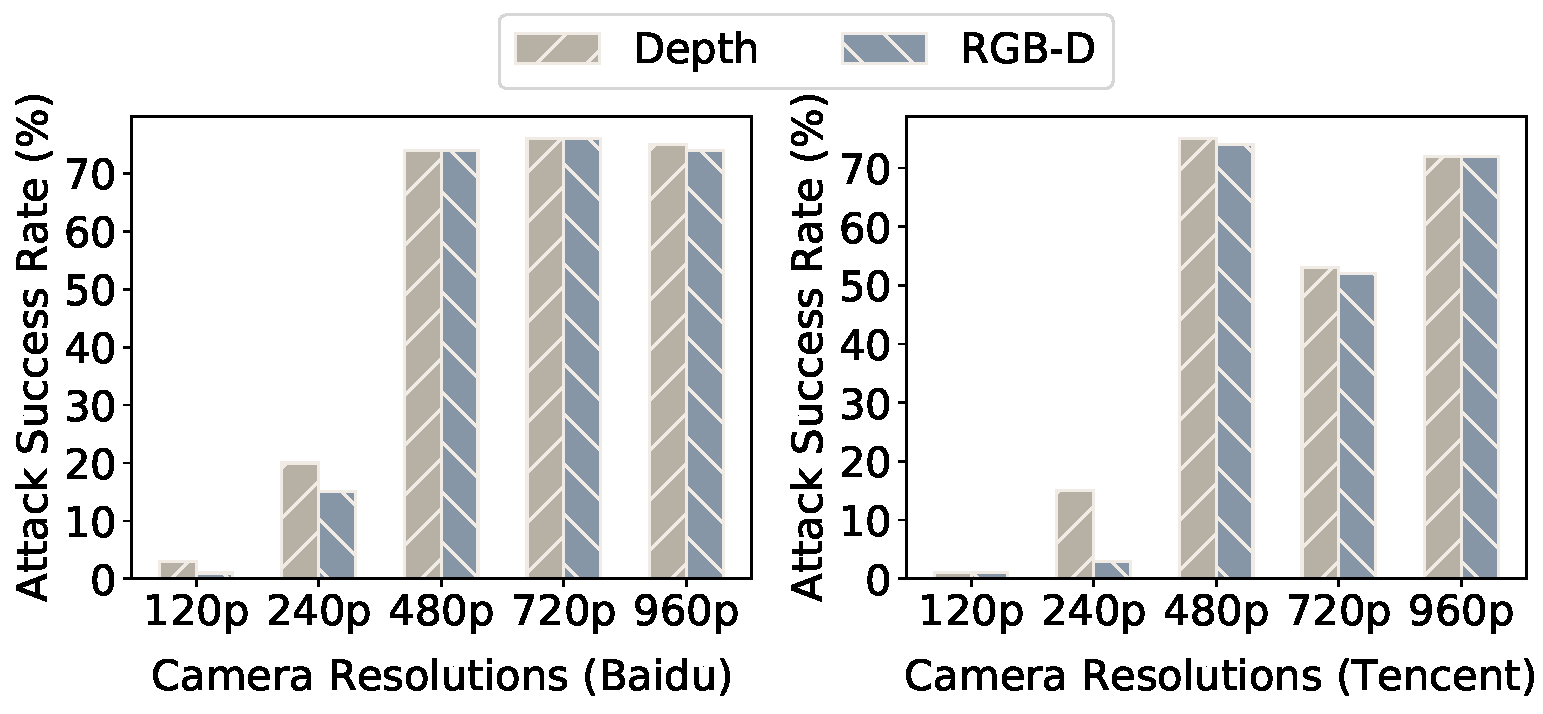
\includegraphics[width = 0.48\textwidth]{figures/camera_resolution.pdf}}
	\vspace{-0.05in}
	\caption{The attack effectiveness of \texttt{DepthFake} attacks under various camera resolutions.}
	\label{camera_resolution}
	\vspace{-0.15in}
\end{figure}


\begin{figure*}[pt]
	\centerline{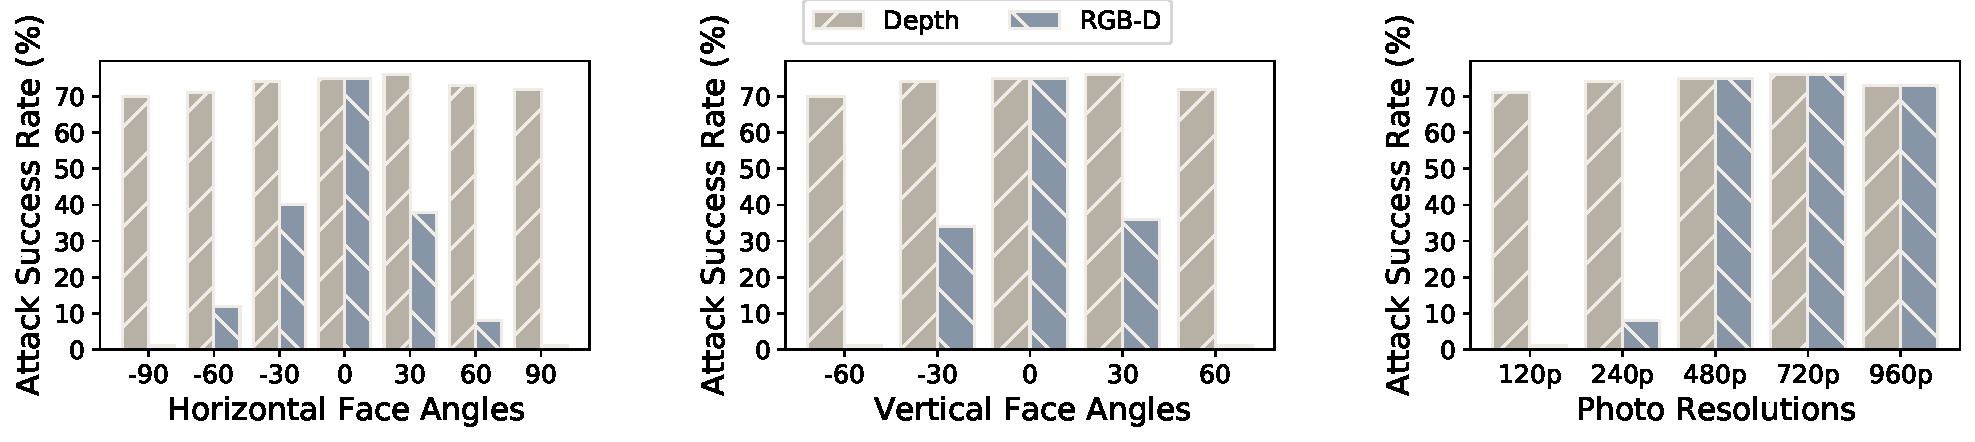
\includegraphics[width = \textwidth]{figures/photo_quality.pdf}}
	\vspace{-0.15in}
	\caption{The attack effectiveness of \texttt{DepthFake} attacks under various photo qualities. }
	\label{photo_quality}
	\vspace{-0.15in}
\end{figure*}


Then, we evaluate the light condition that may influence the attack effectiveness of \texttt{DepthFake}, including the illumination intensity and the color temperature. During the experiments, we use Tencent Cloud SDK with default thresholds as our target system and one volunteer as the victim.  
To avoid the mutual interference between the light intensity and color temperature, we keep the color temperature to $6500~K$ when evaluating the impact of the illumination intensity, and keep the illumination intensity to $300~lx$ when evaluating the impact of the color temperature.

\textbf{Illumination Intensity.} To investigate the impact of the illumination intensity on our attack, we set the background illumination intensity from $50~lx$ to $400~lx$ to conduct experiments.
From the results shown in Fig.~\ref{light_condition} (left), we find that both the Depth attacks and the RGB-D attacks can achieve average attack success rates of over $70\%$.
When the illumination intensity drops to $100~lx$, the attack success rate of the RGB-D attacks shows a slight decrease.
The reason is that the camera suffers from more noises when capturing images at a low illumination intensity. Another finding is that the attack performance at $50~lx$ is better than that of $100~lx$. It is because the camera will compensate for the exposure when the illumination intensity is too low.
At the same time, the attack success rate of the Depth attacks remains $\geq$$70\%$ across different illumination intensities. The reason is that the structured light depth camera uses an infrared scatter pattern to generate depth information, which is not subject to the interference from visible lights.


\textbf{Color Temperature.} Similar to illumination intensity, our attack may be affected by the color temperature. To investigate its impact, we conduct experiments by setting the background color temperature from $3000~lx$ to $6500~lx$.
The results are shown in Fig.~\ref{light_condition} (right). From the results, we find that the attack performance of both the Depth and RGB-D  attacks are unaffected as the color temperature changes, with attack success rates higher than $70\%$.
%The results of RGB attacks are shown in Fig.~\ref{color_temp} (a). From the results, we find that the attack success rates under the default threshold (0.4) reach $99\%$ in different color temperatures. With higher thresholds of 0.6 and 0.8, the attack success rate decreases as the color temperature rise, indicating that the RGB adversarial photo performs better at low color temperatures.%The attack success rate in $3000~K$ color temperature can reach over $90\%$ under a threshold of 0.8, 
%The results of RGB-D attacks are shown in Fig.~\ref{color_temp} (b). Similar to the illumination intensity, the color temperature of visible lights does not impact the performance of depth replay attacks. The RGB-D attacks can achieve an average attack success rate of $44.1\%$ with a depth threshold of 0.5.

Therefore, for the impact of light conditions, we find that (1) lighting conditions have an effect on RGB-D attacks, but almost no influence on Depth attacks because they are based on infrared lights, and (2) \texttt{DepthFake} attacks can achieve an attack success rate of over $70\%$ under most light conditions.

\subsection{Impact of Camera Resolution} 
Commercial face authentication systems may use cameras of various resolutions to capture images, which may influence the performance of our attack. To study its impact, we conduct experiments by using cameras of different resolutions including 120p, 240p, 480p, 720p, and 960p. During the experiments, we employ Tencent Cloud and Baidu Cloud as our victim systems, where the former uses the entire image for detection while the latter only uses the face region. 

From the results shown in Fig.~\ref{camera_resolution},  we find that the attack success rates of both the Depth and RGB-D attacks against two victim systems decline  when the camera resolution drops to 240p. The reasons are: 
(1) For depth images, the lower camera resolution may cause the forged depth image to lose the 3D geometry structure of the human face.
(2) For RGB adversarial photos, the reduction in camera resolutions can weaken the attack effectiveness of the adversarial perturbations. 
%For instance, if the resolution is reduced from 480p to 120p, the face area will be compressed to a quarter of its original size. Thus, the face geometry can be lost and the $5\times5$ pixel adversarial units may also be compressed to one pixel or less, making them easily interfered by noises during imaging.

In addition, we find that with a camera resolution of 720p, the attack success rate against Tencent Cloud is lower than that of Baidu Cloud. The reason is that 720p images use a aspect ratio of $16:9$, while 480p images (default resolution) use $4:3$. Since Tencent Cloud uses the full image  for detection, the change in the aspect ratio will make the image different from the printed adversarial example, leading to a decrease in the effectiveness of the RGB attack. On the contrary, Baidu Cloud uses the face area for detection, which is not affected by the aspect ratio since the face area ratio is fixed.

Therefore, \texttt{DepthFake} attacks work better with cameras with high resolutions. However, with today's trend of using high-resolution cameras for surveillance, we assume \texttt{DepthFake} attacks still has its threat in the real world.

%\begin{figure}[pt]
%	\centering
%	\subfigure[Impact of camera resolutions (Baidu)]{
%		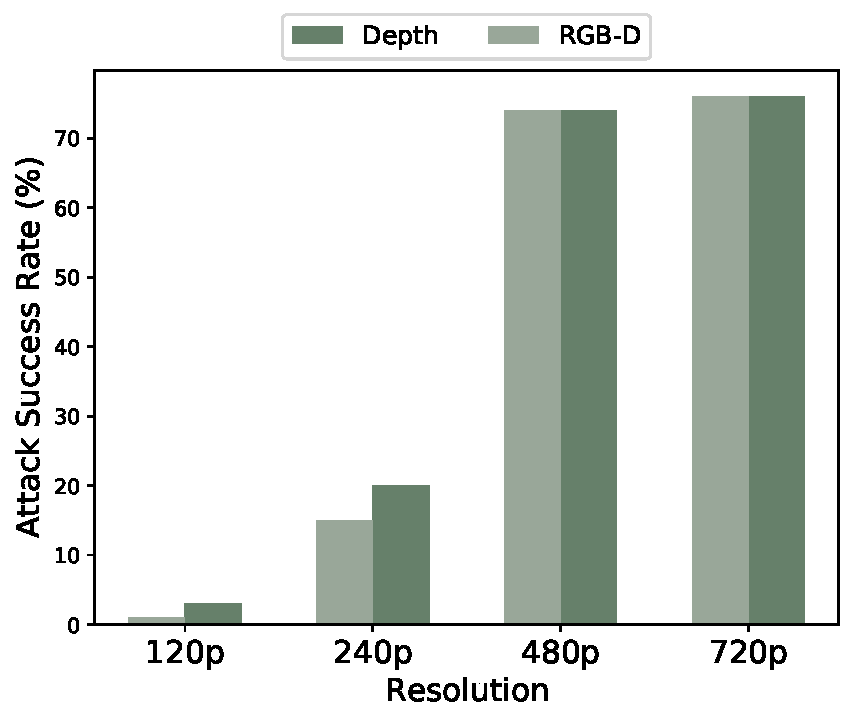
\includegraphics[width=0.22\textwidth]{figures/resolution_rgb_baidu.pdf} 
%	}
%	\hfill
%	\subfigure[Impact of camera resolutions (Tencent)]{
%		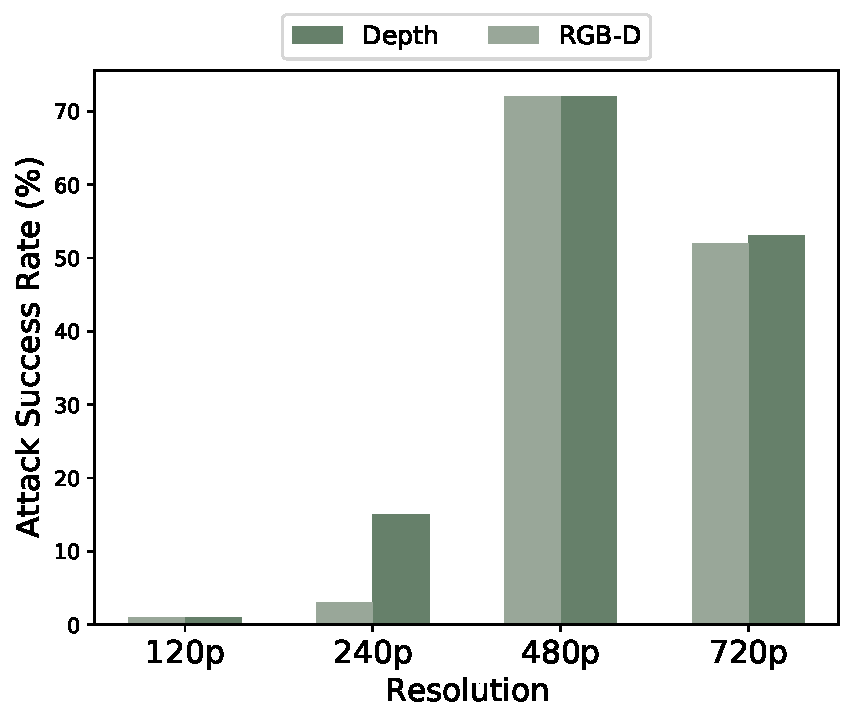
\includegraphics[width=0.22\textwidth]{figures/resolution_rgb_tencent.pdf} 
%	}
%	\vspace{-0.1in}
%	\caption{The attack effectiveness of \texttt{DepthFake} under various camera resolutions.}
%	\label{resolution}
%	\vspace{-0.1in}
%\end{figure}

\subsection{Impact of Photo Quality}
The public photos we obtained from victims' social medias are usually with different face angles and resolutions. In this subsection, we evaluate the attack effectiveness of our attacks under photos with different face angles and resolutions.

%\begin{figure}[pt]
%	\centering
%	\subfigure[Impact of face angle in horizontal]{
%		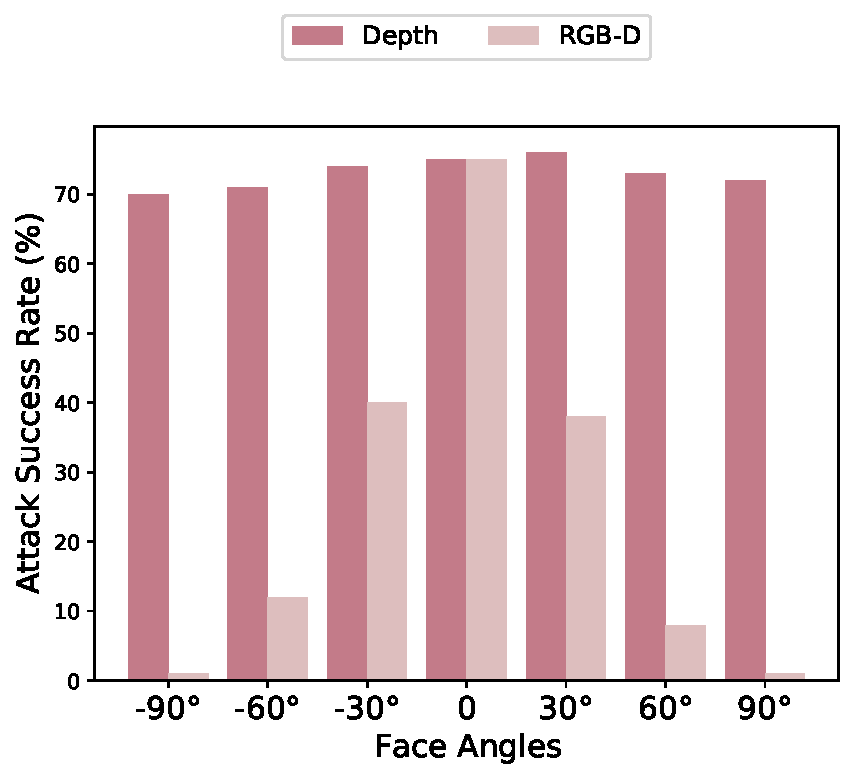
\includegraphics[width=0.22\textwidth]{figures/face_angle_horizontal.pdf} 
%	}
%	\hfill
%	\subfigure[Impact of face angle in vertical]{
%		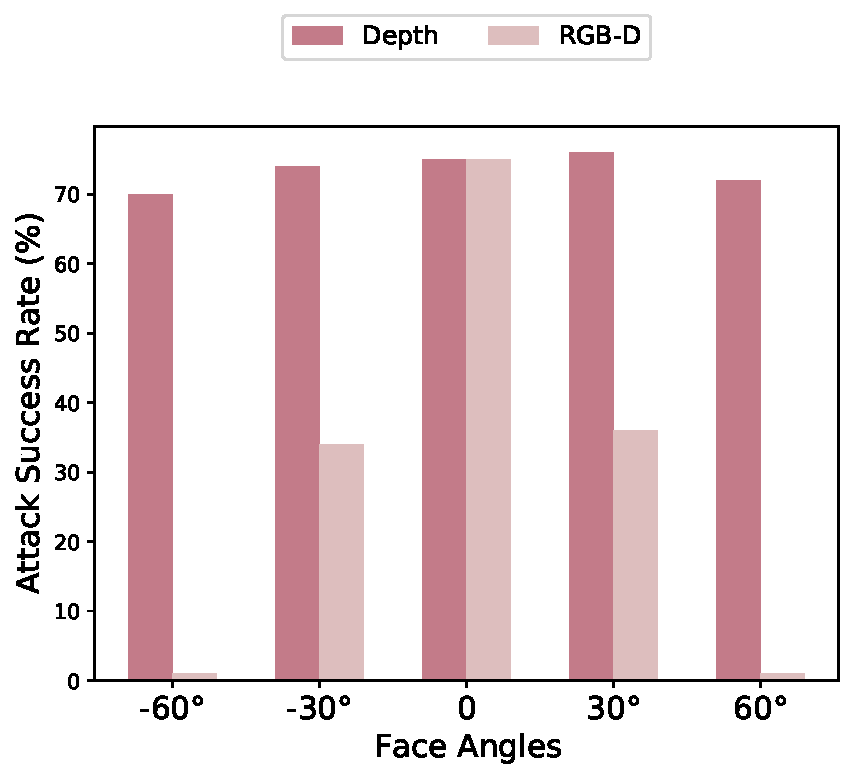
\includegraphics[width=0.22\textwidth]{figures/face_angle_vertical.pdf} 
%	}
%	\vspace{-0.1in}
%	\caption{The attack effectiveness of \texttt{DepthFake} under various face angles.}
%	\label{face_angle}
%	\vspace{-0.1in}
%\end{figure}

\textbf{Face Angles.}
To investigate the impact of face angles, we use images with different face angles in both horizontal (from $-90^\circ$ to $90^\circ$) and vertical  ($-60^\circ$ to $60^\circ$) directions to conduct experiments. 
%The face angles in the horizontal direction are from $-90^\circ$ to $90^\circ$, and the face angles in the vertical direction are from $-60^\circ$ to $60^\circ$.

The results are shown in Fig.~\ref{photo_quality}. For the depth attack, we find that the attack success rate can achieve over $70\%$ at any face angle. 
For the RGB-D attack, the attack success rate is susceptible to the face angle.
For both the horizontal and vertical directions, the attack success rate can achieve over $35\%$ when the face angle is between $-30^\circ$  to $30^\circ$. However, when the face angle is larger than $60^\circ$, the performance of the RGB-D attack decreases.
The reason is that when the face angle increases, the facial information contain in the photo decreases, increasing the difficulty of the RGB adversarial attack and thus the RGB-D attack.



%\begin{figure}[pt]
%	\centering
%	\subfigure[Impact of Photo Resolution]{
%		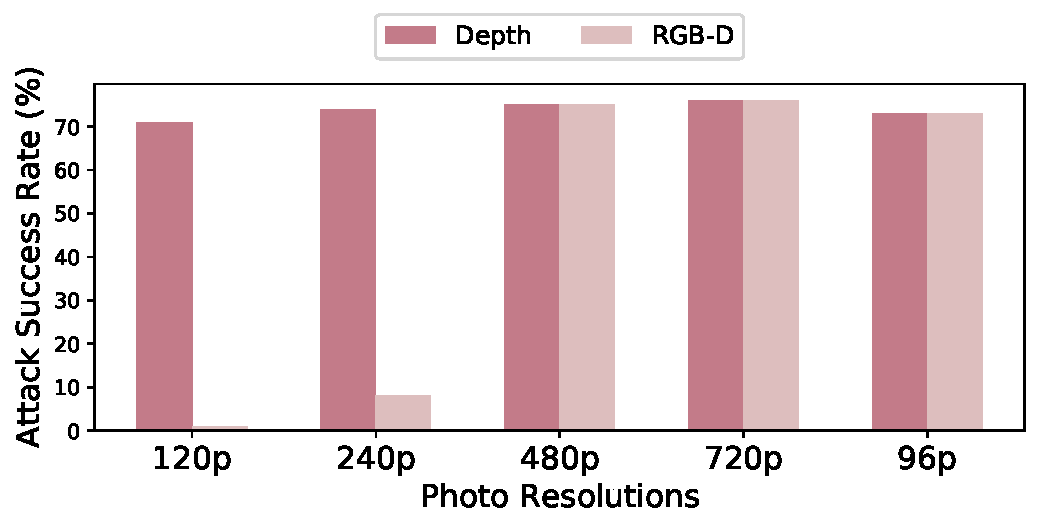
\includegraphics[width=0.45\textwidth]{figures/photo_resolution.pdf} 

%	}
%	\vspace{-0.1in}
%	\caption{The attack effectiveness of \texttt{DepthFake} under various photo resolution.}
%	\label{photo_resolution}
%	\vspace{-0.1in}
%\end{figure}

\textbf{Photo Resolutions.}
To evaluate the impact of photo resolutions, we use photos with different resolutions, i.e., 960p, 720p, 480p, 240p, and 120p, to conduct experiments. From the results shown in Fig.~\ref{photo_quality}, we find that both Depth and  RGB-D attacks can achieve attack success rates over $70\%$ on photos with resolutions larger than 480p. 
However, when the image resolution drops to 240p, the performance of the RGB-D attack decreases.
The reason is that the RGB-based liveness detection model can detect the blurred images and output them as 'non-living'. 
For the Depth attack, it is not affected by low image resolutions since: (1) In the depth estimation phase, our training dataset contains various resolution photos, which makes the depth estimation model robust to low-resolution photos. (2) In the depth forgery phase, the scatter pattern we modulate is not related to the resolution of the original RGB photo.

Therefore, \texttt{DepthFake} attacks work better with  public photos with face angles $\leq 30^\circ$ and image resolutions $\geq$480p.


\subsection{Impact of Relative Position}

\texttt{DepthFake} attacks use an external infrared projector to project the forged scatter pattern to an adversarial photo to launch RGB-D attacks. As a result, the relative position between the camera and the projector may distort the scatter pattern and thus influence the depth generation. In this subsection, we evaluate the attack effectiveness of Depth and RGB-D attacks under different camera-projector distances.

\textbf{Horizontal Distance.} We put the projector $2~cm$ above the camera and change their horizontal distance from  $0~cm$ to $12~cm$ to evaluate the impact of horizontal distances. From the results shown in Fig.~\ref{realted_position} (top), we find that the attack success rates for both the Depth and RGB-D attacks drop as the horizontal distance increases. 
With a horizontal distance of $4~cm$, both the Depth  and RGB-D attacks can achieve attack success rates of about $70\%$. However, when the relative horizontal distance is larger than $6~cm$, the attack success rate is reduced to $30\%$. The reason is that the depth generation highly depends on the location of the scatter pattern. The severe perspective distortion caused by the long horizontal distance will shift the projected scatter, resulting in the attack performance decrease. 

\textbf{Vertical Distance.} To evaluate the impact of vertical distances, we set the horizontal distance between the projector and camera to be  $0~cm$ and change its vertical distance from $2~cm$ to $8~cm$. The minimal vertical distance is set to $2~cm$ instead of $0~cm$ since the 3D camera has a shell of $2~cm$.The results shown in Fig.~\ref{realted_position} (bottom) demonstrate that the performance of the Depth attack and the RGB-D attack declines as the vertical distance increases. Nevertheless, both the Depth and RGB-D attacks can achieve  attack success rates over  $60\%$ when the vertical distance is less than $5~cm$. 
% It indicates that the depth generation of the structured-light camera is more sensitive to vertical distortion. 

Therefore, \texttt{DepthFake} attacks can tolerate a horizontal or vertical distance within $5~cm$ between the projector and the camera.



\begin{figure}[pt]
	\centerline{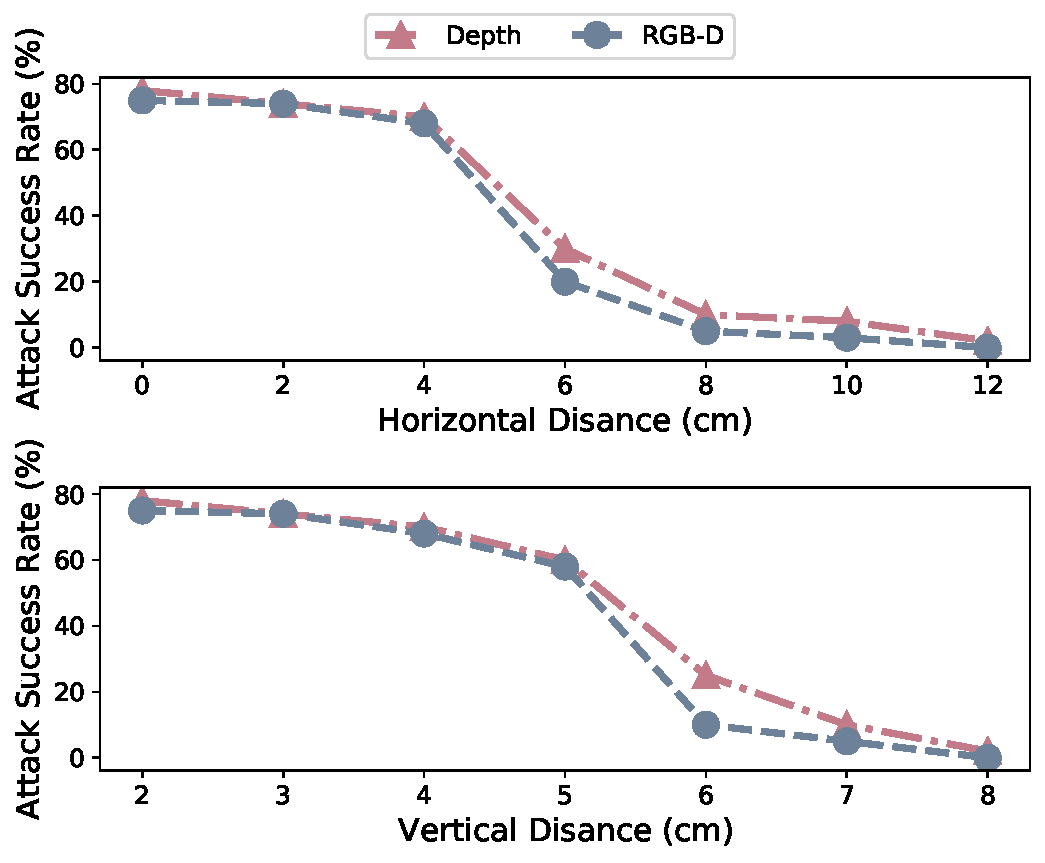
\includegraphics[width = 0.48\textwidth]{figures/related_position.pdf}}
	\vspace{-0.1in}
	\caption{Impact of relative positions between the camera and projector on \texttt{DepthFake} attacks. }
	\label{realted_position}
	\vspace{-0.1in}
\end{figure}


%\begin{figure}[!t]
%	\centering
%	\subfigure[Impact of hrizontal distances.]{
%		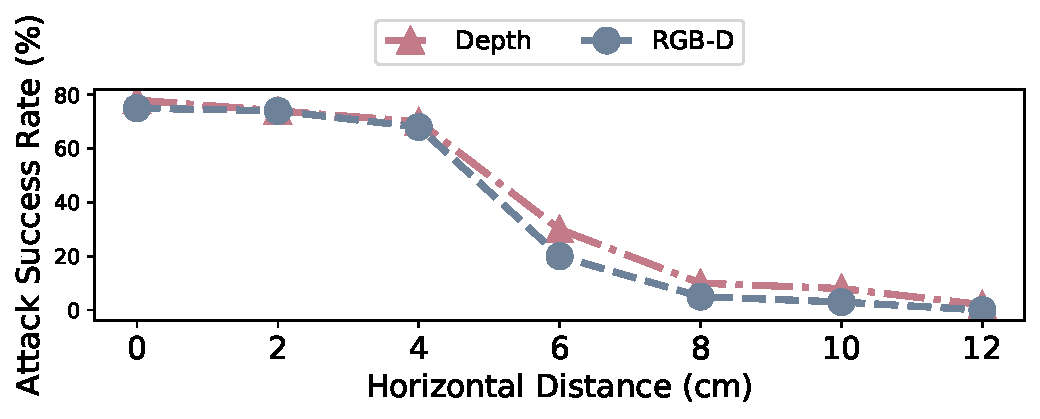
\includegraphics[width=0.45\textwidth]{figures/position_horizontal.pdf} 
%	}
%	\subfigure[Impact of vertical distances.]{
%		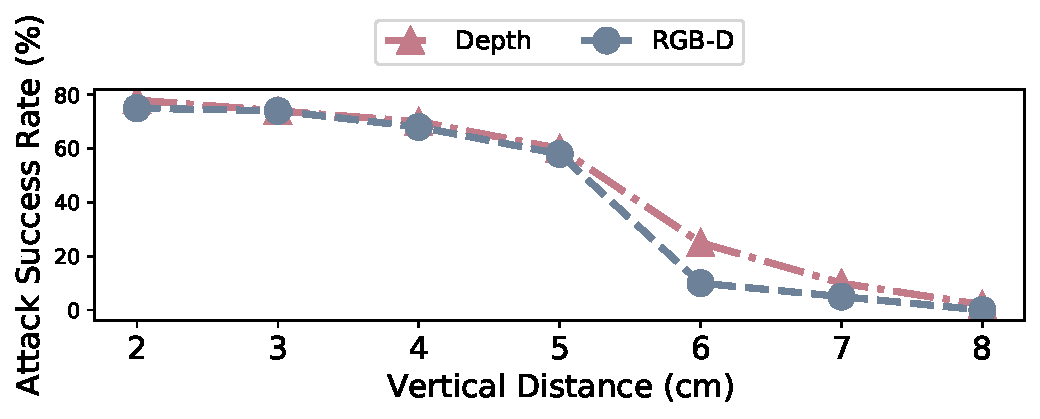
\includegraphics[width=0.45\textwidth]{figures/position_vertical.pdf} 
%	}
%	\vspace{-0.15in}
%	\caption{Impact of relative positions of the camera and projector on \texttt{DepthFake} attacks. }
%	\vspace{-0.2in}
%	\label{Position}
%\end{figure}

\subsection{End-to-End Face Authentication}

The \texttt{DepthFake} attack targets the 3D liveness detection module in the commercial face authentication systems, based on the hypothesis that if we bypass the 3D liveness detection,  the face authentication system can be spoofed with a single photo.
To verify it,  we conduct experiments against end-to-end face authentication systems. Specifically, we evaluate the attack effectiveness of \texttt{DepthFake} attacks against each module in the standard workflow of face authentication systems, including face detection, liveness detection, and face comparison. 

We conduct an experiment with five users against three face authentication systems with their default thresholds.
For the results shown in Tab.~\ref{end2end}, we find that \texttt{DepthFake} attacks can pass every step of the face authentication system and successfully spoof the entire system. Moreover, we find that once the liveness detection step is bypassed, the following face comparison step can be $100\%$ spoofed. The reason is that \texttt{DepthFake} attacks do not make any changes to the face presentation features of the legitimate user. Furthermore, most commercial face authentication systems only rely on RGB images for face comparisons. The adversarial perturbation units we generate are small and sparse, and thus do not affect the face comparison step.


\begin{table}[pt]
	\caption{Attack Effectiveness of \texttt{DepthFake} attacks on  end-to-end face authentication systems.}
%	\vspace{-0.15in}
	\begin{center}
		\setlength{\tabcolsep}{3.5mm}{
			\renewcommand{\arraystretch}{1.2} 
			\begin{tabular}{c|c|c|c}
				\hline
				\multirow{3}{*}{\textbf{Target Systems}} & \multicolumn{3}{c}{\textbf{Workflow of Face Authentication System}}  \\
				\cline{2-4}
				& Face       & Liveness   & Face      \\
				& Detection & Detection    & Comparison     \\
				\hline
				\hline
				Tencent Cloud & 100\% & 71.3\% & 100\%   \\
				\hline
				Baidu Cloud  & 100\% & 63.8\% & 100\%  \\
				\hline
				3DiVi      & 100\%& 72.3\% & 100\%  \\
				\hline
		\end{tabular}}
		\label{end2end}
	\end{center}
	\vspace{-0.15in}
\end{table}


%\subsection{Case Study: Entrance Guard System}
%To showcase the performance of our work on commercial devices in the real world, we validate our attack on an entrance guard device called \textit{Dumu CM Mini}. The \textit{Dumu CM Mini} is deployed with the Baidu Cloud SDK and uses RGB-IR modalities for liveness detection. Thus, we can transfer the RGB adversarial example from the attack against Baidu Cloud SDK. We put the printed adversarial example for RGB modality attack and use projector to relay the infrared image for IR modality attack. 
%
%The authentication result is shown in Figure.~\ref{commercial device}. Before we launch our attack, the \textit{Dumu CM Mini} rejects the access request and raises the access exception. Then, we replace the adversarial photo and turn on the infrared projector for RGB-IR replay attack. As shown in Figure.~\ref{commercial device} (b), our attack successful pass the access request to the \textit{Dumu CM Mini}. It is demonstrated that our attacks can transfer to commercial devices and our attack can be a serious threat to real-world Entrance Guard Systems.
%
%\begin{figure}[htbp]
%	\centering
%	\subfigure[Before attack]{
%		\includegraphics[width=0.225\textwidth]{figures/dumu_1.png} 
%	}
%	\subfigure[After attack]{
%		\includegraphics[width=0.225\textwidth]{figures/dumu_2.png} 
%	}
%	\caption{Performance on commercial device. }
%	\label{commercial device}
%\end{figure}
% !TEX root = ../main.tex
%-------------------------------------------------------------------------------
\section{Case Study: Access Control Device}
%-------------------------------------------------------------------------------
In this section, we evaluate the effectiveness of \texttt{DepthFake} attacks on a commercial access control device in the real world as a case study.



\subsection{Experimental Setup}
\textbf{Target Device.} We analyze a commercial access control device Baidu Rattlesnake Application Kit equipped with Baidu Face Authentication SDK and an Orbbec Astra depth camera, which has been used in airports, metros, banks and other critical infrastructures in China~\cite{baidu_customer}.
The liveness detection module is set to RGB-D mode with default thresholds  (i.e., RGB:0.5, Depth:0.5).

\textbf{Attack Devices.} For Depth attacks, we use an infrared projector DLP4500SL02 Evaluation Module and place it on the top of the camera with a distance of $20~mm$. For RGB attacks, we use a $400~mm\times300~mm$ printed adversarial photo of the legitimate user and place it in front of the target device with a distance of $500~mm$, as shown in Fig.~\ref{setup_2}.

% \subsection{Attack Methodology}
%The \texttt{DepthFake} attack consists of two steps: (1) modulating the desired scatter pattern from the victim's photo and generating the RGB adversarial example, and (2) launching the RGB-D attack to spoof the target device.

%For the scatter pattern modulation, we first use an infrared camera to extract the template scatter pattern of the target device. Then, we obtain the victim's photo, estimate its depth information and modulate it to the desired scatter pattern. 
%For the RGB adversarial attack, we use the victim's photo to generate the adversarial example, then print and put it in front of the target device. 

\subsection{Attack Performance}
We conduct experiments with the Baidu Rattlesnake Application Kit on five legitimate users.
Before experiments, we first generate the users' modulated structured light scatter patterns and their RGB adversarial photos.
During attacks, we cover the scatter projector of the target depth camera, and use the infrared projector to project the modulated scatter pattern on the printed adversarial photo. Then, the depth camera will feed the captured RGB and depth images into the face authentication system of the target device, and  output the authentication results.

An illustration of the real-world \texttt{DepthFake} attack against the commercial access control device is shown in Fig.~\ref{compare}. The results show that 3D liveness detection can defend the naive photo replay attack, but is not effective when against the \texttt{DepthFake} attack. 

To illustrate the effectiveness of \texttt{DepthFake} attacks quantitatively, we launch attacks for 1000 frames per user, and record the attack success rate and the max continuous attack success frames.
As shown in Tab.~\ref{commercial_asr}, we find that our attack is effective against five users, and can achieve an average attack success rate of $60.64\%$. 
Meanwhile, the results demonstrate that our attack can succeed over 6 continuous frames, indicating the feasibility of our attacks against  commercial products utilizing multiple frames for liveness detection.

\begin{figure}[pt]
	\centerline{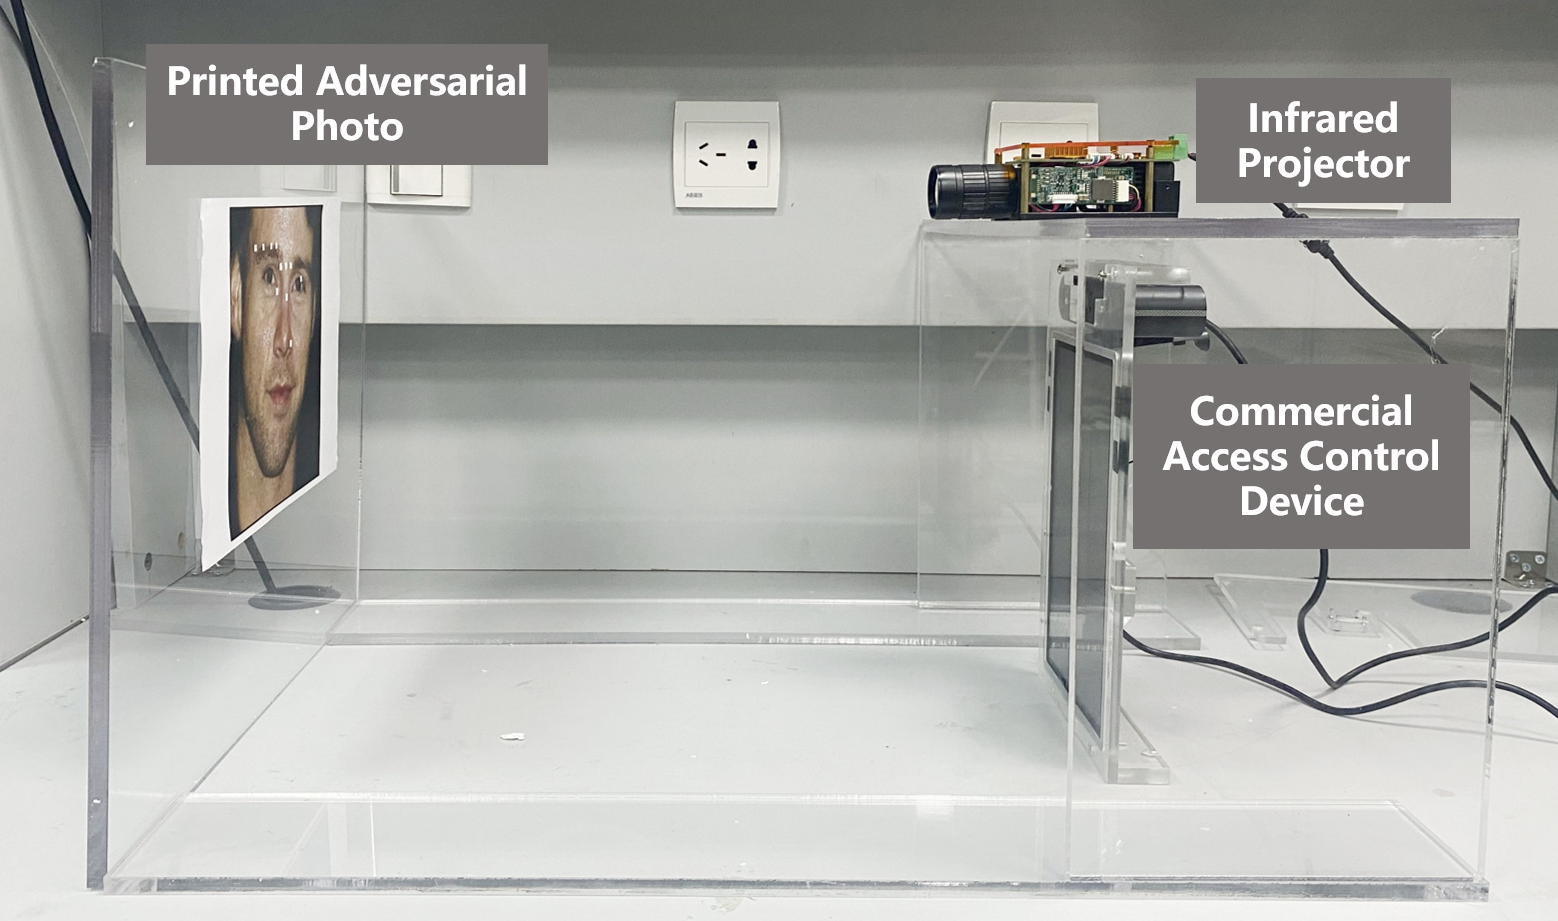
\includegraphics[width = 0.48\textwidth]{figures/commercial_setup.png}}
	\vspace{-0.1in}
	\caption{Experimental setup on commercial access control device.}
	\vspace{-0.15in}
	\label{setup_2}
\end{figure}
\begin{figure}[pt]
	\centerline{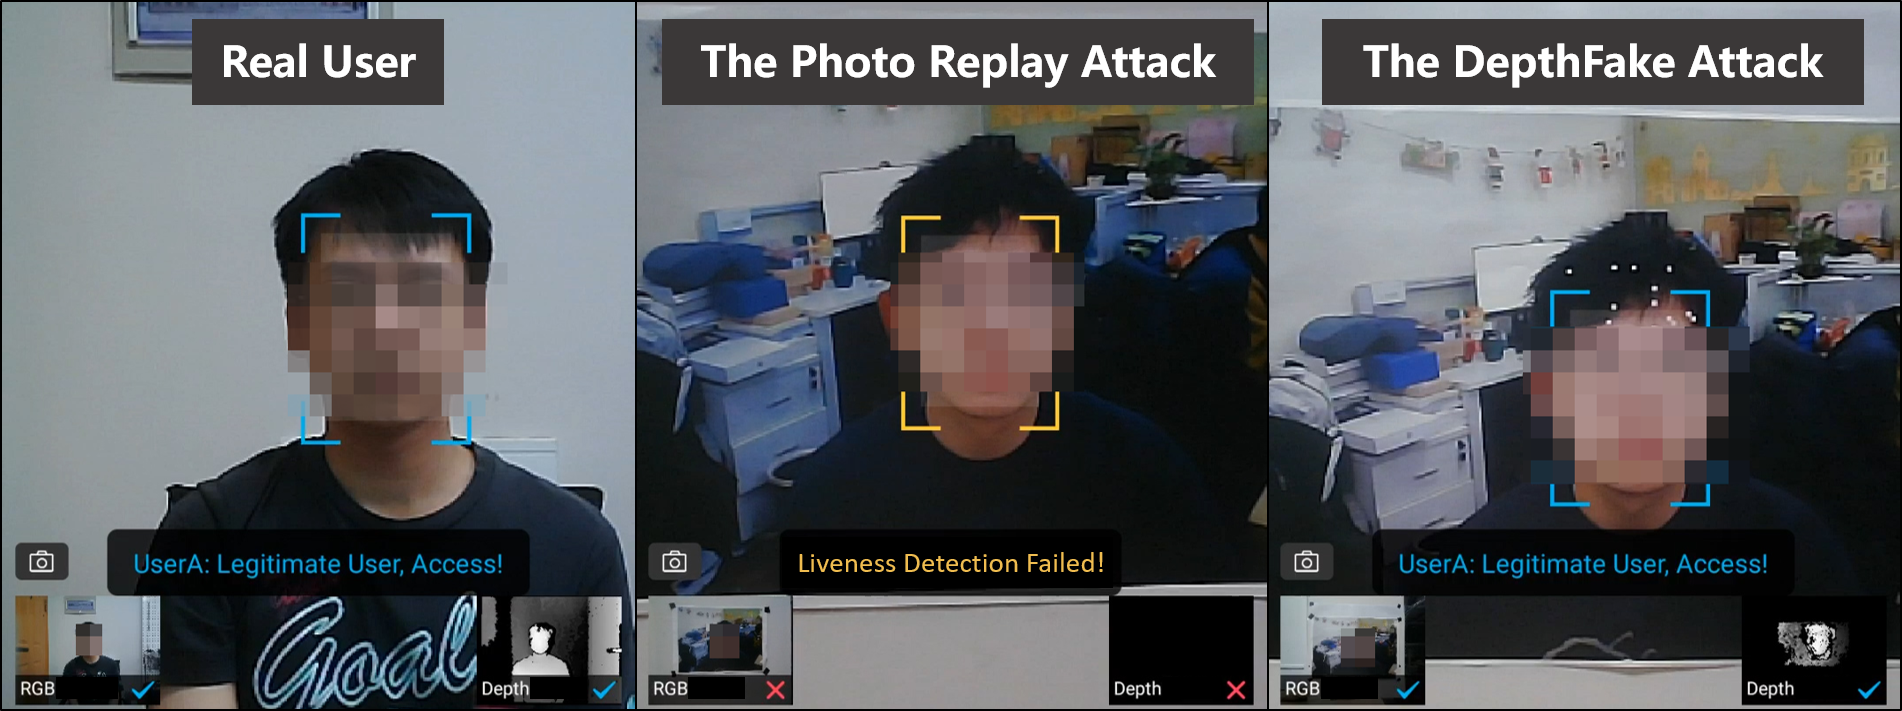
\includegraphics[width = 0.48\textwidth]{figures/commercial_compare.png}}
	\vspace{-0.1in}
	\caption{An illustration of the face authentication results on the real user, the photo replay attack and the \texttt{DepthFake} attack.}
	\vspace{-0.15in}
	\label{compare}
\end{figure}

\begin{table}[pt]
	\caption{Attack Effectiveness of \texttt{DepthFake} on a Commercial Access Control Device}
	\vspace{-0.15in}
	\begin{center}
		\setlength{\tabcolsep}{2mm}{
			\renewcommand{\arraystretch}{1.2} 
			\begin{tabular}{c|c|c}
				\hline
				\textbf{Victim Users} & \textbf{Attack Success Rate} & \makecell[c]{\textbf{Max Continues Frames}\\ \textbf{Under Attack}} \\
				\hline
				\hline
				Person A & $52.2\%$ & 9\\
				\hline
				Person B & $62.4\%$ & 12\\
				\hline
				Person C & $61.1\%$ & 15\\
				\hline
				Person D & $45.5\%$ & 6\\
				\hline
				Person E & $82.0\%$ & 26\\
				\hline
		\end{tabular}}
		\label{commercial_asr}
	\end{center}
	\vspace{-0.15in}
\end{table}

%-------------------------------------------------------------------------------
\section{Discussion}
%-------------------------------------------------------------------------------
%The \texttt{DepthFake} attack identifies vulnerabilities that spoofs the 3D liveness detection module in face authentication systems.
 In this section, we discuss the potential countermeasures and limitations against the \texttt{DepthFake} attack.
%Then, we present the countermeasures and limitations of \texttt{DepthFake}.

%\subsection{IR Replay attack}
%\texttt{DepthFake} exploits the vulnerabilities from the 3D liveness detection module in the face authentication system. However, commercial liveness detection may use the IR image as an auxiliary modality for anti-spoofing~\cite{li2019dual, jiang2020face, liu2021face} due to its low cost. The IR-based liveness detection identifies the real face by comparing the differences in reflected features between real human faces and other spoofing materials. Since \texttt{DepthFake} uses an infrared projector for depth replay, it can also be used for IR replay. We have also validated the feasibility of the IR replay attack in the aforementioned commercial face authentication systems. 

%\textbf{Setup.} Similar to the experimental setup in Sec.~\ref{sec:experimental}, we use the infrared camera of the Orbbec Astra Pro 3D camera to capture an IR image of a legitimate user, and use the infrared projector DLP4500SL02 Evaluation Module to replay the IR image. The tested liveness detection SDKs or APIs including Baidu Cloud, Tencent Cloud, and ArcFace.

%\textbf{Methodology. } We spoof two types of IR-based liveness detection methods supported by the aforementioned SDKs or APIs, i.e. IR-only and RGB-IR. For the IR-only liveness detection, we capture an infrared image of a legitimate user and replay it onto an infrared reflecting plane. Then, we use the infrared camera to capture the replayed infrared image and feed it to the liveness detection module to evaluate the attack effectiveness. For the RGB-IR liveness detection, we replay the infrared image of the legitimate user onto the RGB adversarial photo with face alignment and then feed both the RGB  and IR images to the liveness detection module.  

%\textbf{Results. } As shown in Tab.~\ref{ir_replay_tab} in the Appendix, under the default threshold, the IR replay attack can achieve average attack success rates of $100\%$ and $85.1\%$
%against the IR-only and RGB-IR liveness detection in the aforementioned face authentication systems, respectively. 
%The results indicate that IR replay attacks can simulate the reflected infrared features of real human faces well and IR-only liveness detection is more vulnerable compared with those RGB-based ones.



\subsection{Countermeasure}

\textbf{Detection Model Improvement. } \texttt{DepthFake} attacks exploit the vulnerabilities of the deep-learning-based RGB liveness detection algorithms.
As a result, liveness detection methods with handcrafted features, e.g., LBP~\cite{de2012lbp, boulkenafet2015face}, SIFT~\cite{patel2016secure}, SURF~\cite{boulkenafet2016face}, and HOG~\cite{komulainen2013context}, may help increase the robustness of the model and thus defend our attacks. 

\textbf{Adversarial Examples Detection.} \texttt{DepthFake} attacks utilize the adversarial photos to attack the RGB liveness detection. 
%Since the adversarial perturbations are added to the original image, it can help to detect adversarial examples by distinguishing natural images from adversarial images.
As a result, adversarial example detection methods such as Feature Distillation~\cite{liu2019feature}, Local Intrinsic Dimentionaloty~\cite{ma2018characterizing}, and DkNN~\cite{papernot2018deep}  may help detect the existence of  RGB adversarial photos and thus our attacks.

\textbf{Depth Area Size Detection. }  \texttt{DepthFake} attacks forge the depth information by projecting the modulated structured light scatter pattern with an infrared projector. Since the commercial infrared projector usually has a limited projection size, it cannot generate depth information covering the entire image. As a result,  the size of the area containing depth information can be detected to help determine whether the system is suffering from \texttt{DepthFake} attacks.

\textbf{Randomized Template Scatter Pattern.}  \texttt{DepthFake} attacks spoof the depth camera by modulating the depth information into the template scatter pattern. As a result, using randomized template scatter patterns can increase the attack difficulty, since the attacker needs to obtain the current template scatter pattern and modulate depth information in time. 
%However, it will increase the cost of the hardware and computational resources of the structured light depth camera.

%\textbf{Image Quality Detection. } Another approach of defense \texttt{DepthFake} is to detect quality of RGB and Depth image. 
%For RGB adversarial examples, we use the face quality detection interface provided by the Tencent Cloud SDK and find that the quality score dropped from 0.98 to 0.83 (the average of four people) after the adversarial attack, which means that the adversarial perturbation can affect the quality of RGB images. However, since the adversarial perturbation is small, the quality score of the adversarial example is still over the default threshold (0.8). 
%For Depth replayed images, there is no quality detection for depth images. However, although the replayed depth image can be effective to spoof RGB-D liveness detection, we observe that there are still some blank holes in our replayed depth images which is quite different from the original depth images. 

%\textbf{Consider infrared replay. }Our IR replay attack can consistently succeed to any target system is because almost all current infrared-based liveness detection algorithms do not consider IR replay attacks. If defenders can extract features from the IR replay attack to defend our attack, or update the model by using IR replay images as negative samples, the effectiveness of our attack would be greatly reduced.

\subsection{Limitation}
Our attack has the following limitations at present. 
First, our attack targets RGB-D  liveness detection as it is the most common method for 3D liveness detection nowadays. However, some commercial products may use liveness detection of other modalities such as the IR-D liveness detection. In this case, our attack shall be extended to include the IR-D attack by using the infrared projector to replay the IR images.
Second, our RGB adversarial photo is optimized based on the confidence score of the RGB liveness detection, which may not always be available on commercial devices. In this case, we shall try to generate adversarial photos by using transfer-based black-box optimization methods.
Third, the portability of our attack can be further improved. We will explore using portable attack devices such as mini infrared projectors to make our attack more flexible and practical. 
\textcolor{red}{Lastly, while our attack has yielded good performances when using only a single 2D photo, using multiple victim photos to fuse depth images of various face angles can help to improve face depth estimation accuracy, and further increase the attack performances.}
We remain the aforementioned issues as our future work.
%First, as the first attempt, even though we have proved the feasibility of spoofing commercial 3D liveness detection SDKs and APIs with our RGB-D attacks, we have not
%conducted end-to-end attacks towards commercial face authentication devices.
%Second, our adversarial photos are optimized based on confidence scores, which may not always be available on commercial devices. As a result, our attack algorithms shall be further improved to incorporate such cases.
%Third, we spoof the depth camera by modulating the structured light scatter pattern recorded from the victim user at present. However, if we can estimate the depth information of the victim's face from a 2D photo by using 3D reconstruction techniques and generating a structured-light scatter pattern based on it, the cost of our attack can be further lightened.

\section{Related Work}

In this section, we summarize the related work on face spoofing attacks, including adversarial attacks against face authentication systems and spoofing attacks against depth sensors.

\subsection{Adversarial attacks against face recognition systems}
In the earlier time,  adversaries use photos~\cite{chakka2011competition, anjos2011counter}, videos~\cite{raghavendra2015presentation}, and 3D masks~\cite{bhattacharjee2018spoofing, nesli2013spoofing}, a.k.a., facial presentation attacks, to spoof face authentication systems, which however can be well detected and defended by today's deep learning algorithms. 
Deep-learning-based face authentication systems are effective in detecting those facial presentation attacks yet vulnerable to adversarial attacks, and much prior work has demonstrated the feasibility of spoofing face authentication systems with adversarial examples in both digital and physical worlds.

\textbf{Digital adversarial attacks} usually employ subtle adversarial perturbations at the pixel level, and spoof face authentication systems without human perception. Compared to white-box attacks, black-box ones are more challenging. In this area, DFANet~\cite{zhong2020towards} applied adversarial examples to black-box models by using the transferability of the adversarial attacks. Dong et al. \cite{dong2019efficient} proposed an evolutionary optimization method to generate adversarial faces against decision-based black-box models.

\textbf{Physical adversarial attacks} focus on their capabilities to be deployed in the real physical world.  In this area, the adversarial patch draws much attention since pixel-level adversarial perturbations are difficult to achieve in the physical world. %Advhat~\cite{komkov2021advhat} proposed an adversarial patch taped to a hat that can spoof the face authentication system in the physical world. 
A common method is to attach or print the adversarial patch on wearable stuffs such as  eyeglasses  ~\cite{sharif2016accessorize,singh2022powerful}, face masks~\cite{zolfi2021adversarial}, hats~\cite{komkov2021advhat}, stickers~\cite{guo2021meaningful}, etc, to spoofing face authentication systems.
%Guo et al. ~\cite{guo2021meaningful} disguised adversarial patches on the face as stickers, making them more stealthy when attacking.
Another method is to use external light sources to produce adversarial patterns. Nguyen et al.~\cite{nguyen2020adversarial} projected adversarial patterns onto faces to impersonate or obfuscate targets. Vla~\cite{shen2019vla} projected
adversarial perturbations onto the full face and composed a face with the target features.


Compared with prior work that mainly focuses on spoofing the face comparison step, our work tries to fool the face authentication system with a printed photo of a legitimate user by bypassing its liveness detection step.


\subsection{Spoofing attacks against depth sensors} 
Common depth sensors that can acquire information about the depth of a target including structured light depth cameras,  stereo cameras, LiDARs, etc.
In the area of spoofing depth sensors, much work has been done on the LiDAR~\cite{cao2019adversarial, sun2020towards, tu2020physically} by actively emitting laser signals and utilizing the vulnerability of its deep learning algorithms.
DoubleStar~\cite{277102} exploited the weakness of the stereo matching and used it to manipulate the drone, but it can only produce coarse-grained fake depths. 
Our work is the first one to spoof structured light depth cameras and can forge fine-grained depth information. In addition to the face authentication system analyzed in this paper, our work can be extended to other systems equipped with structured-light-based depth cameras.
\section{Conclusion}

In this paper, we investigate the possibility of feasibility 3D face authentication systems with a single photo and find the key is to bypass its 3D liveness detection module.
% Meanwhile, we find a carefully designed scatter pattern can spoof the structured light depth camera to capture forgery depth information. 
Therefore, we propose the \texttt{DepthFake} attack, which estimates the depth information from a single photo, modulates it to a structured light scatter pattern, and projects such a scatter pattern  on the adversarial photo of a legitimate user to spoof the 3D face authentication system.
Evaluation with three commercial face authentication systems (Tencent Cloud, Baidu Cloud, and 3DiVi) and one commercial access control device demonstrates the effectiveness of \texttt{DepthFake}  attacks in the real world. In addition to the face authentication system analyzed in this paper, our work can be extended to other systems equipped with structured light depth cameras. Future directions include exploring the security of the full workflow of face authentication and the security of other depth systems.

\bibliographystyle{plain}
\bibliography{main.bib}

%\clearpage
\setcounter{table}{0}
\appendix


\section{Appendix}

\begin{algorithm}[h]
	%\textsl{}\setstretch{1.8}
	\renewcommand{\algorithmicrequire}{\textbf{Input:}}
	\renewcommand{\algorithmicensure}{\textbf{Output:}}
	\caption{Black-box Adversarial Perturbation Generation}
	\label{alg1}
	\begin{algorithmic}[1]
		\REQUIRE Printing-Capturing Pricess $C[P(\cdot)]$, the legitimate user's RGB image $X$, RGB-based liveness detection black-box model $D$ and its liveness  $Threshold$, perturbation uint size $(w, h)$
		\STATE Capture the printed RGB image $X$ as $Z = C[(P(X)]$
		\STATE Input $Z$ into $D$, and the model returns  face position coordinates$(X_1,Y_1,X_2,Y_2)$ and confidence-score $S_l$. 
		\STATE $Z_{init} \leftarrow Z$
		\STATE $x \leftarrow X_1$
		\STATE $y \leftarrow Y_1$
		\REPEAT
		\STATE $Z_{temp} \leftarrow Z$
		\STATE Update $Z_{temp}$: Set the $Z_{temp}^{(i,j)}$ into $(R,G,B)_{white}$, where $x<=i<=x+w,y<=j<=y+h$
		\STATE Input $Z_{temp}$ into $D$, and get confidence score $S_t$. 
		\IF{$S_t>S_l$}
		\STATE Update $Z \leftarrow X_{temp}$, $S_l \leftarrow S_t$
		\ENDIF
		\STATE $x \leftarrow x+w$ and  $y \leftarrow y+h$
		\UNTIL $S_l>Threshold$
		\STATE $\delta \leftarrow Z-Z_{init}$
		\STATE Map the $\delta$ to original RGB image $X$ to form the digital adversarial example $\widehat{Z}$
		\ENSURE The digital world adversarial example $\widehat{Z}$.
	\end{algorithmic}  
\end{algorithm}

%\begin{table}[h]
%	\small
%	\caption{Attack Effectiveness of \texttt{DepthFake} attacks on RGB-IR based liveness detection models.}
%	%\vspace{-0.in}
%	\begin{center}
%		\setlength{\tabcolsep}{2mm}{
%			\begin{tabular}{c|c|c}
%				\hline
%				\multirow{2}{*}{\textbf{Target System}} & \multicolumn{2}{c}{\textbf{Modalities}}  \\
%				\cline{2-3}
%				& IR-only & RGB-IR \\ \hline \hline
%				
%				 Tencent Cloud & \textit{100\%} (THR:0.4) & \textit{97.7\%} (THR:0.4, 0.5) \\ \hline 
%				
%			Baidu Cloud & \textit{100\%} (THR:0.8) &\textit{61.3\%} (THR:0.8, 0.8) \\ \hline 
%			
%			 ArcFace  & \textit{100\%} (THR:0.7)    & \textit{96.3\%} (THR:0.5, 0.7)\\  \hline 
%
%		\end{tabular}}
%		\label{ir_replay_tab}
%	\end{center}
%\end{table}

\end{document}
